% Sample Dissertation, Thesis, or Document %
%            for use with the              %
%  University of Arizona Thesis Class,     %
%               uathesis.cls               %
%------------------------------------------%

% We'll use the uathesis document class (duh).  The uncommented line
% below will produce a Dissertation, the others would produce a Thesis
% or a Document.  There are other options available to you like turning
% on the copyright statement and replacing the year on the title page
% with a "generated on" stamp (handy for early drafts).  To find out
% what the available options are, take a look into the uathesis.cls
% file and look for the \DeclareOption commands near the top of that
% file.
% There are five copyright options.  Copyright, no copyright, and three
% different Creative Commons licences.  Use the one you want (If you go
% Creative Commons, I (DM) think the CC-BY-ND makes the most sense)  See
% uathesis.cls for the reason why the non-commercial licenses are not
% included.
\documentclass[dissertation, figuresright]{uathesis}

%\documentclass[dissertation,copyright]{uathesis}
%\documentclass[dissertation,CC-BY]{uathesis}
%\documentclass[dissertation,CC-BY-SA]{uathesis}
%\documentclass[dissertation,CC-BY-ND]{uathesis}
%\documentclass[thesis]{uathesis}
%\documentclass[document]{uathesis}

% Package Usage
% These are the packages that we need
\usepackage{graphicx}
\usepackage{eso-pic}

%\usepackage{natbib}	% natbib is available on most systems, and is
					% terribly handy.
					% If you want to use a different Bibliography package, 
					% you should be able to, just change this
					% and the \bibliographystyle command below.  Be warned
					% that you may need to do a little hacking to get
					% the REFERENCES item to show up in your TOC.
\usepackage[authordate, backend=biber, natbib=true, eprint=false, dashed=false, isbn=false]{biblatex-chicago}
\bibliography{thesis.bib} % add a bib-reference file

\addbibresource{thesis.bib} % add a bib-reference file


% Compatibility with the AASTEX package 
% of the American Astronomical Society.
% I COMMENTED OUT LINE 150 OF DELUXETABLE.STY
\usepackage{deluxetable}		% Allows use of AASTEX deluxe tables
\usepackage{aastex_hack}		% Allows other AASTEX functionality.

\usepackage{colortbl}% http://ctan.org/pkg/colortbl

% These are other packages that you might find useful.
% For controlling the fonts, see
% http://www.math.uiuc.edu/~hartke/computer/latex/survey/survey.html
% The following is a nice font set:
%\usepackage{mathtime}			% Times for letters; Belleek math.
%
\usepackage{amsmath}			% AMS Math (advanced math typesetting)
\usepackage{amssymb} 
\usepackage{lscape}			% Used for making fitting large tables in by putting them landscape
\usepackage[tableposition=t]{caption} % NICK ADDED THIS (makes table captions normal size when font set smaller)

%%% Evan added the following
\usepackage{mathtools}
\usepackage{bm}
\usepackage{enumitem}
% \usepackage{units} % includes nicefrac

%%% The following allows dagger footnote on chapter titles
%%% with no number. Useful for designating previously 
%%% published work.
\newcounter{daggerfootnote}
\newcommand*{\daggerfootnote}[1]{%
    \setcounter{daggerfootnote}{\value{footnote}}%
    \renewcommand*{\thefootnote}{\fnsymbol{footnote}}%
    \footnote[2]{#1}%
    \setcounter{footnote}{\value{daggerfootnote}}%
    \renewcommand*{\thefootnote}{\arabic{footnote}}%
    }

\newcommand{\Msun}{\mathrm{M}_{\odot}}
%\usepackage{refs}			
%
% If you are using hyper-ref (recommended), this command must go after all 
% other package inclusions (from the hyperref package documentation).
% The purpose of hyperref is to make the PDF created extensively
% cross-referenced.
\usepackage[hidelinks]{hyperref}

\usepackage{microtype}
\usepackage{siunitx}
\usepackage{dcolumn}
\usepackage{caption}
\usepackage{longtable}
\usepackage{booktabs}
\usepackage{placeins}
\usepackage{float}
\usepackage{colortbl}   
\usepackage{xcolor}   
\usepackage{tabu}  
% https://tex.stackexchange.com/questions/439111/how-to-wrap-around-table-row-width
\usepackage{tabularx}  
\usepackage{ragged2e}
\usepackage{color, colortbl}
% \usepackage[figuresright]{rotating} %https://tex.stackexchange.com/questions/170205/rotate-table-90-degrees-and-stretch-to-fill-whole-page

% Set up some values.
\completetitle{Information-Seeking, Online Search Tools, and The Formation of New Norms in Health Behaviors during the Covid-19 Pandemic}
\fullname{Kelsey Gonzalez}			% Grad college wants your full name here.
\degreename{Doctor of Philosophy}	% Title of your degree.
\degreemajor{Sociology} % Degree major


\begin{document}


% Set up the title page
\maketitlepage{DEPARTMENT OF SOCIOLOGY}{2022}							

% Insert the approval form.  Note that for electronic submission
% of your Ph. D. dissertation, you must bring *two* copies of the
% approval page to your final defense.  These must be signed by
% the committee.  Make two photocopies: one for Pam and the other
% for your records.  Then, bring the two signed originals to the
% graduate college when you submit the final version of the
% dissertation to the University of Arizona.
\approval
{April 11, 2022}		% Defense Date	
{Ronald Breiger}	% Dissertation Director
{Corey M. Abramson}	    % 1st committee member
{Daniel E. Martinez}	% 2nd committee member
{Yotam Shmargad}		% 3rd committee member

% % Include the ``Acknowledgements''
\incacknowledgements{acknowledgements}

% Include the ``Dedication''
\incdedication{dedication}

% Create a ``Table of Contents''
\tableofcontents

% Create a ``List of Figures''
\listoffigures

% Create a ``List of Tables''
\listoftables

% Include the ``Abstract''
\incabstract{abstract}

% Include the various chapters
\begin{refsection} % refsection environment
\hypertarget{intro}{%
\chapter{Introduction}\label{intro}}

% TODO entire dissertation Covid vs COVID vs Coronavirus


This dissertation focuses on how people search for information and how people
rely on this information and to inform their health-behaviors and develop social
norms. Information permeates every facet of human society, from the hordes of
data gathered through digital trace data or the passing gossip between friends.
Human communication and human society are based on the circulation of
information and knowledge. Information can be shared and promoted by others
through information campaigns and consumed by an individual, called information
push, or intentionally sought out by individuals, called information pull
\citep{cybenkoFoundationsInformationPush1999}.

We must understand the information individuals receive and seek out in order
to develop a well functioning society. The information that
one consumes consolidates to create the entire worldview of every individual,
leading to how they understand the world and behave civilly therein. New and
emerging social norms must align with one's worldview to anticipate any sort of 
behavioral change, for better or for worse. 

The importance of reputable information and misinformation was clearly evident
in the recent and ongoing Covid-19 pandemic. While the vaccines against the
Covid-19 virus prevent severe illness, hospitalization, and death, only 60\% of
Arizonans over 12 years old are fully vaccinated against the virus. We know that
people exposed to misinformation are much less likely to receive vaccinations
against the virus \citep{loombaMeasuringImpactCOVID192021}. It is not an
exaggeration to claim that misinformation has been deadly for Arizona
\citep{pathakInfodemicsCOVID19Role2020, greene_murphy21}.

This dissertation on information search and norm development provides clear and
timely social implications for Arizona and the United States. This dissertation
uncovers how norms are created during periods of norm uncertainty and builds the
foundation to theorize and test interventions that promote positive norms in
times of disasters and uncertainty. Specifically, I investigate how local
diffusion leads to social norms through information search which will have
strong implications for the prevention of global polarization and the spread of
misinformation.

In academia and policy, the main focus in research on information has always
been the information that is sent to consumers, seeing people as passive
receivers of information. My dissertation instead focuses on individuals as
active agents in their search for information which helps me uncover the
information individuals are exposed to. By looking at how individuals search, I
aim to identify pain points and focus areas for future interventions in the
misinformation process.

The information that spread to communities in Arizona led to the health
behaviors exhibited today by Arizonans. While the information spread in various
ways, like through diffusion and polarization, it contributed to our newly
established norms in the Spring of 2020 and since. By uncovering how norms were
created during this time of norm uncertainty, my research will contribute to the
recommended interventions to promote effective health-related behavioral norms
before politicization and misinformation occurs. This will create a healthier,
happier Arizona.

\section{Background}

\subsection{Information Flow}
% what happened before this point? 
A critical turning point in the study of the flow information was put forth by
renowned Sociologist Paul Lazarsfeld \citeyearpar{lazarsfeldPeopleChoice1944}.
Lazarsfeld and others theorized that the media did not directly influence the
masses, but that a "Two-Step Flow" was occurring where "opinion leaders"
interpreted messages from mass media and then, in turn, promoted their opinions
to the masses \citep{katzPersonalInfluencePart1955}. The opinion leaders
interpret, explain, and diffuse contents to "opinion followers". From a networks
perspective, "people rarely act on mass-media information unless it is also
transmitted through personal ties" \citep[p. 1374]{granovetterStrengthWeakTies1973}. 
Lazarsfeld \citeyearpar{lazarsfeldPeopleChoice1944}'s first study focused on
politics but follow up studies from \citep{katzPersonalInfluencePart1955} showed
that this model matched information flows beyond the political realm. In
contrast to the one-step flow, where media directly influences the masses,
Lazarsfeld's theory remains in prominence today. While many scholars assumed
that modern micro-targeted marketing strategies would provide evidence for a
one-step flow perspective \citep{bennettOneStepFlowCommunication2006}, many
scholars find that "opinion leaders" (often influencers and celebrities) still
create a two-step flow of information transmission \citep{choi15,
hilbertOneStepTwo2017}.

The spread of information has been thoroughly studied from the prospective
of social networks. Individuals engage with each other and their distributive
ties to create community contexts where norms, beliefs, and values circulate.
Information diffuses through communities and social networks
\citep{fowler2010cooperative, bond_etal12, klarEffectNetworkStructure2017}.
However, "different things spread in different ways and to different extents"
\citep[p. 563]{christakisSocialContagionTheory2013} and information can spread
differently than a virus or behavior. Important studies in the spread of
information through networks include the study of adoption of innovations by
physicians \citep{colemanDiffusionInnovationPhysicians1957}, how new inventions
are adopted from early adopters to laggards
\citep{rogersDiffusionInnovations1962}, how weak ties help bind networks and
diffuse information \citep{granovetterStrengthWeakTies1973}, how social ties
spread information about job opportunities
\citep{granovetterGettingJobStudy1995, montgomeryJobSearchNetwork1992}, how
information spreads best when weak and strong ties are balanced (embeddedness)
\citep{uzziSocialStructureCompetition1997}, and more recent innovations in the
stickiness of complex contagion \citep{centolaComplexContagionsWeakness2007}.

\subsection{Information Search}
I only discussed the way that information is passively
consumed through push efforts by opinion leaders and social networks. However,
sociological literature is really sparse on the opposite behavior: active
directed searching by individuals to obtain information.
\citep{pejtersenDesignComputeraidedUsersystem1984}, a scholar of library and
information science, theorized that there are 5 strategies for searching for
information. The most common strategy is browsing, where people follow leads
based on associations without planning ahead. Another strategy is analytical,
which includes an explicit consideration of all facets of the question to guide
a search. The empirical method guides the search based on tactics that were
successful in past research. The known site strategy is to go to the direct
source of the information if known. And finally, the similarity method is to
find information based on another similar question that already has an answer.
These 5 strategies vary in their demands for prior knowledge, cognitive
processing, memory, and time spent. While this theory is aimed at finding
information in a library setting, scholars have extended the theory to other
fields and validated the framework \citep{fidelHumanInformationInteraction2012};
the frame is a useful beginning point for the theories of information search
through network activation or through computer-mediated communication.

\subsection{Information Search in The Digital Age}

The introduction of the internet and digital technologies introduced an epochal
disruption in the communication and informational-search mediums that people had
available to them. Computer-mediated communication was the largest communication
revolution in a century, changing the speed and availability of communication
between individuals by electronic mail, instant messaging, two-way interactive
video calls, discussion forums, blogs, and social networking
\citep{rainie2012networked}. Computer-mediated communication encompasses any
sort of communication through computers connected to the internet; the umbrella
term involves both synchronous and asynchronous communication as well as
one-to-one, one-to-many, or many-to-many exchanges. Social media, on the other
hand, are more specific, and are "Internet-based, disentrained, and persistent
channels of mass personal communication facilitating perceptions of interactions
among users, deriving value primarily from user-generated content.” \citep[][p.
50]{carr2015social}. While an email between colleagues is computer-mediated
communication, it is not social media as there is only one interaction between
users and there is no value derived from the user-generated content outside the
pair \citep{bayer_etal20}. Even more restrictive still is the social networking
site, which consists of a profile, a network, and a stream or a feed
\citep{boyd2007social, ellison2013sociality,},  often also involving a messaging
component  \citep{bayer_etal20}. Social networking sites are also interesting
because they often uniquely combine one-to-one communication within the context
of one-to-many communication, like resharing a television news story to your
facebook feed and chatting with others about the content in the comments
section. But what do these classifications mean for the information-seeking
behaviors of individuals in the 21st century? Not only is it quicker to perform
network activation and seek support, but people are "permanently online,
permanently connected" making activation easy \citep{vorderer2017permanently}.
The constant connectedness facilitates communication, but also presents people
with overchoice, or the difficulty in making a decision because simply every
network connection you may want to activate is permanently connected and easy to
reach. In other words, constant connection may be debilitating to many who are
seeking information. \citet{smallSomeoneTalk2017} provides many examples of this
when he demonstrates that more often than not, graduate students who needed
support simply asked "miscellaneous classmates encountered down the hall" (p.
176) rather than their trusted, long-term confidants. It seems that network
activation may rely on more than just trust; namely: convenience.

The digital age did not only revolutionize communication. It also
revoluitionized information search \citep{ramirez2002information}. Just as prior
to the digital age you could open an encyclopedia or peruse the library to find
the information you seek, much of the computer-mediated information search
surely occurs outside of social network activation contexts. While searching in
an encyclopedia is far less common today, internet search engines have
revolutionizes the speed and ease at which we can find information. Early web
search engines allowed information seekers to browse web directories and early
engines like Yahoo! and Altavista found success using keyword-based search,
though the early algorithms were limited in what they could find and relied
heavily on the wording of the queries. Google, the major web search engine used
today, introduced the disrputive PageRank algorithm in the early 2000s, securing
its place as the information hegemon of the 21st century
\citep{brin1998anatomy}. Not only has computer-mediated information search
revolutionized the ease of obtaining information, but it has also changed out
brains. \citet{sparrow2011google} show that the digital age has led to worse
memory and higher reliance on technology to keep track of information for us.
These search engines have also shaped our cultures by controlling, whether
through algorithm or intentionally, the information the engine provides. For
example, Google will not show results for various neo-Nazi websies in countries
where holocaust denial is illegal, like France and Germany. This is illustrative
of the control engines have over information and how this control may introduce
various political, economic, and social biases in the information they provide
\citep{segev2010google}. When 99Firms \citeyearpar{99firms22} compiled the data
from sources like NetMarketShare, Statista, DuckDuckGo, Yahoo Finance, Google,
and Pew Research they find that about about Around 93\% of all web traffic is
via a search engine and that 78.39\% of all internet search use Google. Because
computer-mediated information search is instantaneous and only requires mobile
data or wifi, there is virtually no cost to seeking information on one of these
mediums.

\subsection{Theory of Uncertainty Management}

Some communication theorists ask why an answer to a question is sought in the
first place. The Theory of Uncertainty Management
\citep{brashersCommunicationUncertaintyManagement2001} professes that people
search for information when their uncertainty around the subject leads to
anxiety or other cognitive harms. The Theory of Motivated Information Management
\citep{afifiSeekingInformationSexual2006, afifiTheoryMotivatedInformation2004}
extends the prior by adding that uncertainty itself is not the catalyst for
information-search; rather, it is driven by a discrepancy between the current
level of uncertainty on a subject and desired level of uncertainty.




\subsection{Social Support}

One way to find information is to activate network ties to find out information
through a form of social support. Social support, while previously used
interchangeably with the term social networks and social integration
\citep{houseStructuresProcessesSocial1988}, are the emotional, informational,
and instrumental assistance functions performed between social ties and have
strong and measurable association with health outcomes
\citep{houseMeasuresConceptsSocial1985, thoitsMechanismsLinkingSocial2011}.
Informational support is the process of seeking "help in defining,
understanding, and coping with problematic events and include education, advice,
or referral to another source of support" \citep[p. 640]{winemiller_etal93}.
Brashers, a health communications researcher, defines informational support
slightly differently, focusing on the exchange of information that "facilitates
coping with life stresses... that may be exchanged among members of a support
network" \citeyearpar[p. 260]{brashersInformationSeekingAvoiding2002}. Both of
these definitions provide important lenses for my question of how
computer-mediated or interpersonal information-seeking strategies vary. 
Some research has revealed that Facebook users who utilize the platform to 
find information and to maintain relationships have high levels of bridging
social capital \citep{liu2016meta}. However, this leaves the question 
of who activates their social networks for information using social networking 
sites like Facebook over activating these networks in face-to-face interactions. 


\subsection{Uses and Gratification Theory}

From studies of mass communication, uses and gratifications theory (UGT)
\citep{blumlerUsesMassCommunications1974, tanMassCommunicationTheories1985} may
lend itself to theorizing why information-seeking strategies vary among different
platforms and activation types. UGT posits that users are not passive
consumers of media and that people have an active role in choosing different
sources of media based on their satisfaction of specific needs on an individual
basis. UGT is based on Maslow's \citeyearpar{maslowTheoryHumanMotivation1943}
hierarchy of needs and is compatible with Lazarsfeld and Katz's theory of
two-step flow because people can choose their media and the opinion leaders they
follow. Modern-day theorists have extended UGT theory and classified the uses
and gratifications of the internet and of social media.
\citet{staffordDeterminingUsesGratifications2004} theorize that the internet
provides gratification through useful content that meets expectations,
gratification from purposeful navigating or random browsing as a process, and
social gratification from forming and deepening social ties.
\citet{leungGenerationalDifferencesContent2013} theorizes that social media is
gratifying for users because it allows for venting of negative feelings,
provides recognition, provides entertainment, promotes social affection, and
fulfills cognitive needs. 

There has been some research into how different platforms allow for different user 
experiences or "affordances" \citep{boyd2010social}. For example, \citet{bossetta18} first show
that all social media platforms must provide "tools that are easy to use and 
functional to the demands of varying using demographics" (p. 473). They also
explain how each digital architecture enables, contstrains and shapes how users
behave on their platform and in virtual space, leading to many different experiences 
along the dimensions of searchability, connectivity, and privacy. 

Adapting UGT to my own purposes, I theorize that
informational support will be activated from network ties when the informational
need is related to forming and deepening social ties
\citep{baumeister,grieve2013face} but search will be conducted outside of network
activation when information is needed but an individual does not have an additional cognitive
need to fill through social interaction. Alternative goals such as identity
management or relational maintenance
\citep{brashersInformationSeekingAvoiding2002} need to be balanced and may also
influence where search is conducted.

\subsection{Social Norms}
I showed the levels of uncertainty may direct how and when people
search for information. However, in situations of rapidly changing norms,
uncertainty is prevalent. This dissertation will also focus on developing
new social norms in situations of uncertainty about how to behave. 
Minimal research exists in quickly emerging
norms in times of emergency, but shows that people likely to rely on the
behavior of others' to set their own norms for behavior \citep{alvarez2018,
horneNormsIntegratedFramework2020}. This project will investigate how search
contributes to the development of said spontaneous norms.

Social norms form the building blocks of social organization and have been a
focus of sociology since the beginning. In a recent Annual Review of Sociology
piece focused on social norms, Horne and Mollborn define norms as "group-level
evaluations of behavior ... [or] when people have expectations about how others
evaluate behaviors" \citeyearpar[p. 468-69]{horneNormsIntegratedFramework2020}.
One of the principal architects of sociology, \'{E}mile Durkheim, saw that
society exerted powerful forces on individuals and classified people's norms,
beliefs, and values as parts of collective consciousness that provide for
societal integration \citeyearpar{durkheimSuicide1897, durkheimDivisionLaborSociety1933}.
For Durkheim, norms were therefore the glue that held society together in cohesion.

Max Weber, another founding architect of sociology saw social norms differently.
Weber distinguished social behavior from social action, which was an action a
person takes through subjective understanding and interpretation of actions of
others \citeyearpar{weber1978economy}. Weber therefore saw social norms through
the lens of the subjective meanings behind every action. Actions that were not
considered by an individual were not the focus of Weber. New spontaneous norms
that are emerging in a society under upheaval, like the health behaviors that
emerged during the Covid-19 pandemic, emerged with new subjective meanings and
cognitive associations that held consequences for the individuals who adopted
the social actions.

The causes and logics of social norms are debated. The consequentialist
argument for norms focuses merely on the consequence a behavior has on
group members and that norms will be promoted if the behavior benefits
others and denounced if it negatively affects others \citep{ullmannmargalitEmergenceNorms1977}.
 While this theory has been tested and performs well in the lab,
researchers have raised questions regarding its ecological validity
\citep{horneNormsIntegratedFramework2020}. One of the main critiques of the
consequentialist argument is that it relies on the same interpretation of the perceived action
by all parties of what is harmful and beneficial. The Relational argument 
for norms is based on the value people place on their relationships and
the assumption that people will behave in ways that will garner them
positive social reactions. This argument relies on individuals assuming
what their peers will approve and disapprove of. In turn, norms are
developed when individuals make inferences from their social worlds
\citep{fryeCulturalMeaningsAggregation2017}.

Importantly, people look to others performing an action and often
interpret that performance as an indication that an action is approved,
paying particular attention to high-status individuals and institutions
\citep{robalinoPeerEffectsAdolescent2018, tankardEffectSupremeCourt2017}.

\subsection{Social Networks}

Norms are formed inside of social networks; "Networks operate in a larger cultural
context that can facilitate or inhibit acceptance of general cultural norms and
beliefs" \citep[][p. 44]{pescosolidoDurkheimSuicideReligion1989}. 
Because of this, people tend to resemble
their network as a form of network autocorrelation and homophily
\citep{dellapostaWhyLiberalsDrink2015}. While "birds of a feather flock
together" in homophily \citep{mcphersonBirdsFeatherHomophily2001}, attitudes and
behaviors are shaped by peers, creating filter bubbles of social influence
\citep{dellapostaWhyLiberalsDrink2015}.

\citet{goldbergSocialContagionAssociative2018} argue that the state of the
literature on diffusion and social contagion, discussed above, is erroneous.
They propose an important linkage that had been missed in previous research of
the diffusion of behavior (or, as I interpret it, the creation of new norms).
They argue that what actually diffuses during social contagion are the
perceptions about which beliefs or behaviors are compatible with one another,
what they call "associative diffusion". 
This relates back to the theory of relational norms, where individuals assume
what their peers will approve and disapprove of. In order for these assumptions 
to take place, they must have an understanding of which behaviors and beliefs
are possessed by whom in their network and how new associations may influence
or disrupt the expected actions. 
In times of behavioral uncertainty, I
theorize that individuals strategically look towards other high-status
individuals, institutions, and perform regimented searches to establish for
themselves the behavior that is compatible with other cognitive biases they
hold.

\section{Broader Impact}
\begin{center}
    \texttt{UNDERGOING CHANGES}
\end{center}

% TODO make Broader Impact more relevant to actual findings
% Original

This research will first and foremost impact sociology. While the spread
of information is investigated in the discipline (diffusion, mass
communication, social influence), it is almost always from a structural
perspective which disregards individual agency and choice in the
acquisition of new information. This perspective aligns with Uses and
Gratifications Theory, discussed in Section B: Background, and sees
people as active agents in their search for information instead of just
passive receivers of information signals.

Taking this agentic perspective is critical in the study of information
diffusion when combined with cognitive perspectives like that of
Goldberg and Stein (2018). How people search for information determines
the information that they find; the information they uncover is filtered
through cognitive biases and predispositions to how they interpret and
act upon the newfound information. Searching for informational support
through social network ties theoretically will uncover potentially
different information than that would be uncovered through online web
search and will change how people are organized and how people behave.

Additionally, this dissertation will investigate how social norms are
formed in situations of uncertainty, an area that is less developed in
sociology. While sociologists have studied social norms since the
formation of the discipline, focus on the quick formation of social
norms has implications for social behavioral outcomes, cultural change,
organizational reactions to unrest and disasters, and many more areas
that influence humanity.

This dissertation will also have implications for the study of social
networks and social support. Not only is this work situated in the
sociological study of social support and social influence, but I utilize
rarely-used-in-sociology sources of big data to better understand these
mechanisms and test existing theories.

This dissertation also contributes to computational social science \&
critical big data studies. I base much of my dissertation around Google
Search Trends, which are relatively underutilized in the social sciences
compared to health sciences and business. Not only does this project
introduce Google Search Trends in new ways, but I perform explicit tests
of how this data should be used in the social sciences, providing the
groundwork for this exciting source of big data for future computational
social scientists. Because my research takes a critical big data studies
approach, I take into account the potential pitfalls with any source of
big data (McFarland and McFarland 2015) and attempt to explicitly answer
questions posed by this field, such as "what are the behavioral
processes that lead to macro-level outcomes" proposed by \citet{breigerScaling2015}.

I also make important contributions to social epidemiology through this
research. Each of the three papers in this dissertation use health case
studies for questions of sociological interest. Because of this, I will
contribute to social epidemiological questions on vaccine hesitancy,
health communication, and diffusion of high-risk health behaviors. While
all of these areas are important to social epidemiology, there are
potential important health implications for these contributions on
outside of the academy.

Outside of the academic research impacts that this dissertation makes,
there are clear and timely social implications that will stem from this
work. First, by uncovering how norms are created during norm
uncertainty, I may be able to establish recommendations for
interventions to be applied during disasters and other times of unrest
to promote effective positive norms. Second, my research may have
implications for how to optimize gratifications in search processes to
promote healthy social relationships and improved online algorithm
deployment.

This work also relates to polarization and misinformation, two major
social issues of our time. \citet{axelrodDisseminationCultureModel1997} shows that network structure,
autocorrelation, and diffusion create local convergence of attitudes and
culture which then leads to global polarization \citep{dellapostaWhyLiberalsDrink2015}. In investigating how local diffusion leads to social norms
through information search, some of my findings may have strong
implications and interventions for the prevention of global
polarization. Relatedly, understanding where and how people search for
information has implications for the information they are exposed to and
the norms they develop. This project will attempt to relate to where
misinformation is uncovered and how to intervene in its absorption.

\section{Three Empirical Articles}

\begin{center}
    \texttt{all three of these are UNDERGOING CHANGES}
\end{center}


\begin{figure}
{\centering 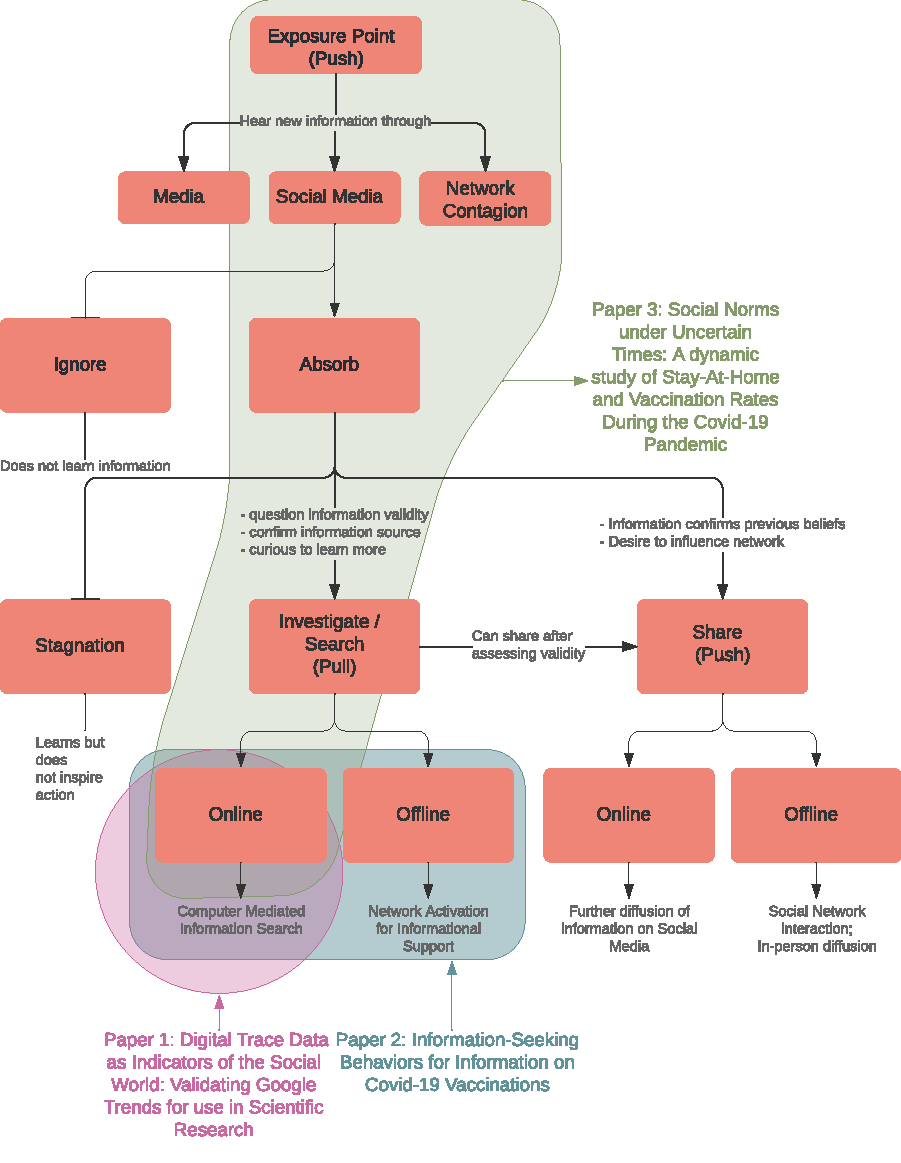
\includegraphics[width=\linewidth]{figs/ch1/Dissertation Concept Map - Color.pdf}}
\caption{Theoretical Framework for the Dissertation}\label{fig:concept-map}
\end{figure}

To make my intended contributions to the literatures on computational
social science, sociological methodology, social norms, social networks,
and diffusion, my dissertation will take the following format:

% todo, go over fig:conceptmap


\hyperlink{paper-1}{\subsection{Article 1: Digital Trace Data as Indicators of the Social World: Validating Google Trends for use in Scientific Research}}

- How can we operationalize Google Search Trends as a valid indicator for uses in social science research?    


I will first investigate how Google Search Trends can be operationalized
as cultural attitudes, disease prevalence and voting behaviors through
comparing trends data to observed valid indicators of these cases.
Specifically, I will test cultural indicators from the NORC General
Social Survey, United States county-level suicide rates from National
Center for Health Statistics, US case rates of Covid-19 from The New
York Times, historical US Presidential Election results, and the
American National Election Survey against selected Google Trends terms
and analyze the data using correlation methods. The aim of this article
is to assess the construct validity and will contribute to critical big
data studies and sociological methodology.

Computational social science and other disciplines are quick to 
adopt new sources of digital trace data for use in academic research. 
In this article, I examine the validity of Google Search Trends 
as potential indicators of three different cases, namely attitudes, 
disease prevalence and political preferences using eight %TODO double check number
different validated data sources. I use Pearson and Repeated Measures Correlations 
between the Google Trends and the validated indicators as well as multiple linear regression
(for cross-sectional datasets) and random intercept hierarchical linear models
(for longitudinal datasets) as additional tests of the data. 
I fail to find correlation among any of the Google 
Trends tested and their validated indicators. While some Google Trends 
tested were significantly associated with the outcome in the regression models,
effects tended to be small and the total model interpretability remained low,
even when controlling for demographic variables. This article shows that there is no 
external validity of Google Trends for these uses and social scientists
will find no replacement for high quality survey data with Google Trends. 

\hyperlink{paper-2}{\subsection{Article 2: Information-Seeking Behaviors for Information on Covid-19 Vaccinations}}

- How do computer-mediated or interpersonal information-seeking strategies vary
across populations?
- What factors lead people to perform health information search on the Covid-19 vaccine online versus among social network ties? 

The second article in my dissertation investigates the question "what
are the behavioral processes that lead to macro-level outcomes" (in this
case, Google Trends results) proposed by \citet{breigerScaling2015}. Knowing that
Google trends data only encompasses a small portion of the
information-seeking done by modern humans, it is important to
investigate what leads individuals to search for a question online using
a search engine (contributing to macro-level trends data) versus more
traditional means of information gathering, such as network activation
(asking someone in their social network for informational support). To
investigate this, I use the case of receiving, requesting, and sharing
information about the Covid-19 vaccine in a survey I received funding to
conduct of 900 Adults in the United States.

Previous research has greatly failed to distinguish between the activation of
information seeking behaviors online and offline. Using theories of social
support and uses and gratifications theory I investigate the factors associated
with each vehicle type when on information seeking vehicle: personal connection,
doctor, social networking site, online forum, and online search engine. Using
novel survey data of % TODO  nrow(rain) Americans and their experience seeking out
information about the Covid-19 vaccines, I find little evidence that online
search is more utilized than seeking social support from personal network
connections or health professionals. I find evidence that the vehicles queried
in this survey are conceptually different and that the utilization of different
vehicles varies by demography and information sources. Finally, I find that
different fountains of information and information search vehicles hold real
world consequences through their associations with Covid-19 vaccination rates
and intentions, as information from a doctor increased the Covid-19 vaccination
uptake while receiving information from a Social Networking Site like Facebook
or Twitter was associated with lower odds of vaccination.  



\hyperlink{paper-3}{\subsection{Article 3: Social Norms under Uncertain Times: A dynamic study of Stay-At-Home and Vaccination Rates During the Covid-19 Pandemic}}

- How are new health behavior norms regarding public health recommendations formed during the Covid-19 pandemic?  
- How are patterns of information-search related to social norm stabilization during the Covid-19 pandemic?  

My final article takes a deeper dive into the formation of social norms
governing health behaviors in cases of extreme uncertainty using the cases of
both a) population mobility during early 2020 and b) vaccination rates during
early 2021, both as responses to public health recommendations to mitigate the
Covid-19 pandemic. Using theories of associative diffusion and the integrated
theoretical framework of norms, I test how these health behaviors are outcomes
of assortative signaling from networks and other sources, such as social
isolation and connection between communities, religious and political
conservativism, and attention to media sources, and online norms as measured by
information-search behaviors. To investigate this, I conduct statistical
modelling on a dataset I compiled from multiple sources, including Google,
Facebook, and the Center for Disease Control and Prevention.

This paper examines how social norms are formed under conditions of uncertainty
using the case studies of stay-at-home and vaccination rates during the Covid-19
pandemic.  I test fear-based models of behavioral adaption to public health
recommendations as well as patterns of complex social contagion using linear
mixed effects models. These models show that complex contagion is a valid
framework for the social contagion of new norms during Covid-19. However, I find
important moderating effect of signal discordance, the contextual diversity of
signals received by an ego.

\newpage
\section{References}
\begin{singlespace}
\printbibliography[heading=none] % print section bibliography
\end{singlespace}
\end{refsection}

% Include the various appendices
\appendix

\begin{refsection} % refsection environment
\hypertarget{paper-1}{%
\chapter{Digital Trace Data as Indicators of the Social World: Validating Google Trends for use in Scientific Research}\label{paper-1}}

\section{Abstract}

Computational social science and disciplines such as sociology and
political science are often quick to adopt new sources of digital 
trace data for use in academic research. 
In this article, I examine the validity of Google Search Trends 
as potential indicators of three different cases, namely attitudes, 
disease prevalence and political preferences using five
different validated data sources. I use Pearson and Repeated Measures Correlations 
between the Google Trends and the validated indicators as well as multiple linear regression
(for cross-sectional datasets) and random intercept hierarchical linear models
(for longitudinal datasets) as additional tests of the data. 
I fail to find correlation among any of the Google 
Trends tested and their validated indicators. While some Google Trends 
tested were significantly associated with the outcome in the regression models,
effects tended to be small and the total model interpretability remained low,
even when controlling for demographic variables. This article shows that there is no 
external validity of Google Trends for these uses and social scientists
will find no replacement for high quality survey data with Google Trends. 

\textbf{Keywords}: Google Trends, Social Science Methodology, Digital Trace Data, Information-Seeking Behavior, Information and communications technology, Validity

\section{Introduction}

New sources of digital trace data have led to vast possibilities for social science
research because they are bigger, cheaper, and already available 
\citep{kingEnsuringDataRichFuture2011,lazerComputationalSocialScience2009,salganikBitBitSocial2017}.
Digital trace data are the expansive volumes of information that are now available with the
introduction and widespread adoption of the internet and include sources such as  
social media sites, search data, blogs, adminstrative data on websites, the internet 
archives, etc. In short, digital trace data are the crumbs that are left as a person
peruses and interacts in digital spaces. Scholars have noted that these data provide
many new research avenues for social scientists because they are always on, non-reactive to
a researcher's observation, and very often captual social interactions and relationships,
but warn they can be Inaccessible, Non-Representative, and be prone to drifting due to
algorithmic confounding \citep{salganikBitBitSocial2017}.
Before overenthusiastically embracing these
sources and integrating them into our big data toolkits, social scientists must clearly establish
parameters under which these data sources are appropriate, 
and for which questions they are useful 
\citep{bailCulturalEnvironmentMeasuring2014, lazerParableGoogleFlu2014}. As
prior research outlined, the "quantity of data does not mean that one
can ignore foundational issues of measurement and construct validity and
reliability and dependencies among data" 
\citep[p. 1203]{lazerParableGoogleFlu2014}. 

With the expansion of big data, some computational social science research has
developed extremely innovative methods that have led to groundbreaking results using 
reliable sources of big data. As an example,\citet{blumenstockPredictingPovertyWealth2015}
use county-level cell-phone records to construct the distribution of poverty
and wealth in Rwanda, a country where national surveys and censuses are
rare and costly. However, \citet{blumenstockPredictingPovertyWealth2015} go to
great lengths to demonstrate that their use of the cell
phone data creates a reliable and valid construct; few social science
papers utilizing big data dig into the construct validity of their
metrics to this extent and even fewer publications focus on
methodological guidelines of how to use sources of big data
\citep[For exceptions, see ][]{asseoTrackingCOVID19Using2020, stilesAssessingCriterionValidity2018}.
However, research has shown the small adjustments to an algorithm or
metric may void any research insight we can pull from such data
\citep{lazerParableGoogleFlu2014}.

\subsection{Google Trends}

Social scientists have yet to widely utilize Google Search Trends as a source of big data.
Google Trends is a free and publicly accessible data resource
provided by Google, a major internet search
engine worldwide, that analyzes the top search queries across different localities, 
languages, and time. While Google Trends is freely available and holds a breadth of 
online activities that could potentially be of use in social science, few social 
scientists outside of economics have used this resource \citep[see][for examples]{choi2012predicting, jun2018ten,da2011search}. This paper provides evidence-based guidelines for social scientist who would use these resources in their toolboxes on how we can triangulate Google Search Trends
as validated indicators and under what circumstances.

Building on prior research outlining the various issues with different sources of big data
\citep{boydCriticalQuestionsBig2012,lazerIssuesConstructValidity2015},
this paper evaluates the construct validity of Google Search Trends as an indicator of three different
cases, namely attitudes, disease prevalence and political preferences.
These three cases will be tested using attitudinal indicators from the %NORC General Social Survey, 
CDC \citeyearpar{vaches_data} and New York Times \citeyearpar{mask_data}, 
health indicators from the CDC \citeyearpar{suic_data}, 
US cases rates of COVID-19 from The New York Times \citeyearpar{covid_data},  
and political indicators from the historical US Presidential Election results \citeyearpar{pres_data}.
% , and the American National Election Survey \citeyearpar{anes_data}.
This paper will contribute guidance for creating standards of how to use Google
Trends for social research, and identify potential pitfalls that can compromise the 
analysis including the focus of this paper, which shows that Google Trends has a
lack of ecological validity. 


\subsection{Google Trends and research on attitudes}

I will use three categorizations of ways I propose Google Trends could
be utilized for social scientific usage. First, I test Google
Trends as an indicator of attitudinal indicators. 
After \citet{bailCulturalEnvironmentMeasuring2014}'s call for
cultural sociologists to utilize the ever-expanding world of big data,
Google trends began slowly appearing as a data source in sociological and
social science research. From research on mass shootings and firearms \citep{brownsteinInternetSearchPatterns2020, semenzaInformationseekingWakeTragedy2020}, 
protest and anti-Muslim sentiment \citep{bailUsingInternetSearch2018,barrieSearchingRacismGeorge2020,grossThereFergusonEffect2017},
to analyzing country-level changes in social perception \citep{reyes_etal18},
Google search trends are a new and innovative indicator of cultural interest.
Extending into social networks and culture, \citet{bailPrestigeProximityPrejudice2019}
even used Google trends to measure how they saw 'culture' spreads around the globe
through the proliferation of search terms.

\subsection{Google Trends and research on health behaviors}

Google Search Trends have been utilized to estimate disease prevalence
and population throughout the health sciences. While much of this research has focused on
the COVID-19 pandemic \citep{jimenez_etal20, jimenezCOVID19SymptomGoogle2020, limEstimatingInformationSeekingBehaviour2020, mavraganiCOVID19PredictabilityUnited2020, nguyenGoogleTrendsAnalysis2020, todorovaInternetBasedData2021, mingUnderstandingHealthCommunication2021},
other research has investigated Google Trends as indicators of wellbeing
\citep{brodeurCOVID19LockdownsWellbeing2021, carpiTwitterSubjectiveWellBeing2020, duCOVID19IncreasesOnline2020},
suicidality \citep{burnettTimeTrendsPublic2020}, 
vaccination uptake \citep{dalumhansenEnsembleLearnedVaccination2016}, 
obesity \citep{sarigulNowcastingObesityUsing2014}, 
and even insomnia \citep{zittingGoogleTrendsReveal2020},
to cover a few examples. For a partial review of other utilizations, see \citet{nutiUseGoogleTrends2014}. According to \citet{jaidkaInformationseekingVsSharing2021}, the majority of studies profess
a correlation of \> .70 between the IV and DV, "demonstrating the vast potential of Google
Search as a proxy for monitoring population health" (p. 3) based on
assumptions that individuals search because of self-diagnosis and to
identify possible courses of treatment \citep{dechoudhurySeekingSharingHealth2014}.


\subsection{Google Trends and research on politics}

Various sources have also used Google Trends to forecast
political elections and political attitudes
\citep{wolfTrendingRightDirection2018}. For instance,
\citet{swearingenGoogleInsightsSenate2014} investigate how U.S. Senate
Elections relate to attention measured by search traffic.
\citet{pradoromanGoogleTrendsPredictor2020} demonstrate how Google Search trends
successfully predicts presidential election results in both the United
States and Canada. Finally, the OECD Development Centre is investigating
how Google data can help elucidate governments' approval in Latin
America \citep{montoyaUsingGoogleData2020}. Overall, the papers 
cited here find favorable relationships between Google Trends and
voting outcomes and claim that it is also a valid measure of public attention. 

\subsection{Causes for concern}

While Google Trends has not been widely used or validated by social scientists,
I am not the first author to investigate its validity.
Some researchers have cautioned against the wide usage of Google Search Trends. For instance, \citet{asseoTrackingCOVID19Using2020} 
concludes in their research on COVID-19 case rates and Google searches that the correlation 
is often spurious and due to confounding. They even explain that "searches would
result not only from self-symptoms, but also from interest elicited by
media coverage" \citep[][p.1]{asseoTrackingCOVID19Using2020}.

\citet{rovetta21} also investigates the reliability of COVID-19 searches to infer 
the quality of the data; the author finds that there are various issues with missing data in 
smaller regions and significant variation in correlations between the sampled regions throughout
the study period. Rovetta indicates that this is a cause for concern and is undoubtedly due to more 
serious causes than behavioral changes among the population or changes in the underlying product algorithm. 

\citet{cebrian_domenech22} emphasize in their research that there are some 
non-negligible issues with the measurement of Google Trends, pointing to 
errors within the purview of accuracy, completeness, consistency, and validity,
as outlined in \citet{KarrDataQuality}.  
% I know it is basic stats, but I would provide a footnote explaining each of your terms. Here, these line up with mainline stats but disciplines vary.
 \citet{cebrian_domenech22} point not only to 
meta issues like the lack of transparency into the sampling methods 
and population coverage, but they identify real differences 
in the data provided by the Google Trends API for the same 
researcher-entered query, pointing to likely internal process 
used by Google to sample their data to compute the trends.
These authors show that the variability of the results over time for the same query
can alter the results of analysis and forecasting significantly. While the 
issue of unreliability isn't unique to the Google Trends API, 
\citet{cebrian_domenech22} propose 
caution in the use of this digital trace data for other researchers until
further research can determine the root cause for the inaccuracies.
% Yes, big issue. But, it is also seen in machine learning, survey 
% administration, etc. I’d assume one solution for dealing with fiddly 
% output is to just sample repetedly and do some sort of average, 
% perhaps with a correction if the direction of the error is non random.

Finally, it is important to note that most of the research using 
Google Trends as digital trace data do so to indicate
population's \textit{attention} to a search query. Because
% I’d also say, the population is examined differently. It is really a population of action remnants being used to get at a population of people, which is presumed to be represented online.
searches can be done with many different intentions, such as 
information gathering, navigational purposes, etc., it may
be hard to declare that an overall level of engagement with a topic
on Google Search may be indicative of anything more than interest \citep{da2011search}.
To reference Clifford Geertz's invocation of Ryle, we only know that the search was 
performed, not whether it indicated a digital wink or twitch \citeyearpar{geertz1973thick}.
% For a soc audience some sort of reference to the dilemma of interpretation would be interesting.

\citet{jungherr_etal17} explore this topic deeply with data from
Twitter on German federal election candidates and find that there is no
indication that tweets about candidates are indicative of or can predict 
political support. Instead, they conclude that tweets merely indicate the
temporal dynamics of public attention toward politics. The same may
be true about Google Trends. 

Building on this previous research in the reliability and accuracy of the trends, 
it is imperative that we provide a framework for how to use diverse sources
of digital trace data as social scientists. The aim of this paper is
to take the first step to build that framework. I examine the validity of 
Google Search Trends to indicate attitudes, health outcomes, or political 
support using the methods that follow.

\section{Methods}

To test how well Google Trends can be used to indicate other measures, 
I use various tests to validate the criterion validity of the trends. 
Criterion validity measures how well one measure, an operationalization of a 
specific construct, is able to predict a theoretical representation 
of the construct — the criterion. For this article, I employ 
concurrent criterion validity which looks at how Google Trends can
predict various criterions in the same time scale. 
I gathered geo-located social science data across multiple
sources to address the three areas of inquiry for this paper.  Table
\ref{tab:data-sources-table} outlines which data sources I use in this
project and which trends are matched to each source.

\newcolumntype{L}{>{\raggedright\arraybackslash}X}
	
\definecolor{Gray}{gray}{0.9}
\definecolor{lightblue}{HTML}{bad7db}

\renewcommand{\arraystretch}{1.2}

\begin{table}[!ht]
\caption{\label{tab:data-sources-table}Data Sources}
\centering
\fontsize{8}{10}\selectfont
\setlength{\extrarowheight}{2pt}
\begin{tabularx}{\linewidth}{@{}L c c L@{}}
\toprule
\textbf{Validated Data Source} & \textbf{Type} & \textbf{Dates} & \textbf{Google Trends Used}\citep{googletrends} \\ \midrule
% \rowcolor{lightblue}
\multicolumn{4}{l}{\textbf{Behaviors and Attitudes}} \\\hline
% General Social Survey & Cross-Sectional & 2010 - 2020 & NA \\
Vaccine Hesitancy for COVID-19 \citep{vaches_data}& Cross-Sectional & March 3 - 15, 2021 & Search Topics: 'Covid-19 vaccine', 'Coronavirus (Disease)', 'Coronavirus   (Virus)', 'Vaccine' \\
Mask-Wearing Survey Data \citep{mask_data} & Cross-Sectional & July 2 - 14, 2020 & Search Topics: 'Coronavirus (Disease)', 'Coronavirus (Virus)', 'Cloth   Face Mask', 'Mask', 'Civil and Political Rights' \\
American National Election Survey \citep{anes_data}& Cross-Sectional & 2020 & NA \\
% \rowcolor{lightblue}
\multicolumn{4}{l}{\textbf{Health}} \\\hline
Covid Rates \citep{covid_data}& Longitudinal & Every Monday, 2020 - 2021 & 'Covid-19', 'Coronavirus', 'Taste Loss', 'Smell Loss' \\
Suicide Rates \citep{suic_data} & Longitudinal & Yearly 2010-2020 & Search Topics: 'Suicide', 'Depression', Search Term:' Suicide Hotline' \\
% \rowcolor{lightblue}
\multicolumn{4}{l}{\textbf{Political}} \\\hline
American National Election Survey \citep{anes_data}& Cross-Sectional & 2020 & NA \\
Presidential Election Results \citep{pres_data}& Cross Sectional & 2016 \& 2020 & Search Topics: 'Hilary Clinton', 'Donald Trump', 'Joe Biden' \\ \bottomrule
\end{tabularx}
\end{table}










\subsection{Measures}

\subsubsection{Google Trends}
This paper focuses on a triangulation of Google search trends \citep{googletrends}
with other sources of credible data.
Google trends portray the search frequency for specific search terms across
designated media markets areas (DMAs), a nonoverlapping aggregation of U.S.
counties to 210 media markets based on Nielsen's classification o "similar population clusters" \citep{dma_key}.
Raw data is on a scale from zero to one hundred, with one hundred being the maximum search
popularity out of all DMAs. When available, I use Google search topics to
measure trends as opposed to search terms. Search topics are a more robust
measurement than a single search term: topics are aggregations of the rates of
multiple, highly correlated search terms together into a cohesive topic done
by Google through it's Knowledge Graph product. For
example, while 'Beyoncé', 'Beyonce' and 'beyonce knowles' are all separate
search terms, 'Beyoncé Knowles' encompasses all of these into a single search
topic. Google Search Trends are only available cross-sectionally (a single 
period across a geography) or as time-series (a single geo-location across
time). To remedy this and build a longitudinal dataset of each search topic 
to match the longitudinal validated measures, I follow the method proposed 
in \citet[][p. 5]{park_etal}\footnote{This method involves building a dataset of unscaled cross-sectional values,
selecting a DMA to use to establish the rescaling ratio (I use 'Los Angeles
CA'), and then finding the time-series values for the one DMA. To find the
rescaling ratio for each week in the time-series, you divide the time-series
value for each week by the cross-sectional value for each week, resulting in a
rescaling vector to be used for all weeks in the dataset across geographies. To
rescale each longitudinal value, multiply the respective week's rescaling ratio
by the cross-sectional value. To validate this method, I compared the rescaled
longitudinal data against multiple samples of time-series data. For a more
in-depth explanation of this procedure, see \citet[p. 5]{park_etal}}. I interpolate 
missing datapoints in the longitudinal datasets using The Zoo package for R \citep{zoo}.

\subsubsection{Attitudinal}

%  create a  Table People will want to see a Table of variables, their prompts, and ranges.

% <!-- \citep{gss_data} (let's see if I get access first) -->

One measure of attitudinal indicators is the Vaccine Hesitancy for COVID-19
\citep{vaches_data}. The CDC uses the U.S. Census Bureau’s Household Pulse Survey
(HPS) and the 2019 American Community Survey (ACS) 1-year Public Use Microdata
Sample (PUMS) to measure U.S. residents’ intentions to receive the COVID-19
vaccine if available during May 26, 2021 – June 7, 2021. This dataset consists
of 3,148 observations, one for each U.S. County. The variable
measures the percent of adults in the county who describe themselves as
“unsure”, “probably not”, or “definitely not” going to get a COVID-19 vaccine
once one is available to them. The variable ranges from 4.99\% to 32.33\%. 

Another attitudinal indicator I use is the Mask-Wearing Survey Data conducted by
Dynata, a global online market research firm, for the New York Times from 
July 2 through 14, 2020 \citep{mask_data}. 250,000
survey respondents were asked, "How often do you wear a mask in public when you
expect to be within six feet of another person?". The NYT weighted each response
to create a county level measure of what percent of the county never, rarely,
sometimes, frequently, and always wore a mask when in public. This dataset
consists of 3,148 observations, one for each U.S. County included in the sample. This measure
is purposed to estimate the percent of adults in the county who never or rarely wear a mask
(range = 0.10\% to 55.80\%).

\subsubsection{Health}

I also use U.S. COVID-19 rates to validate health and disease related topics. I
retrieve U.S. county-level COVID-19 rates from \citet{covid_data}, who compile this
data based on reports from state and local health agencies. It is widely
acknowledged that there are biases in this data due to inconsistencies and
availability in testing as well as different community propensity to test
%  Also blatant political interference in some places, which is probably worth acknowledging.
\citep{gu22, cdc20a} However, it is the best measure we have of actual case rates
without extensive adjustments.
Case Rate is measured as number of cases per 100,000 population. Observations
vary from a minimum of zero to a maximum of 1460.46 for each Monday from January 27, 2020, through
December 27, 2021. There are 285,986 cases across 3,136 counties and 101
dates. Missing data were interpolated using The Zoo package for R \citep{zoo}.

I also use county-level suicide rates from the US Centers for Disease Control
and Prevention \citeyearpar{suic_data}. Data is grouped by year from 2010-2020. Raw death
rates are scaled by population size for each year and can be interpreted as the
death rate by suicide for every one thousand people. There are 34,683 total
cases, resulting from 10 observations of 3,147 counties. Missing data were interpolated using
\texttt{na.approx()} \citep{zoo}. Measures range from 0.034 to 53.254.

\subsubsection{Political}

Finally, I evaluate Google Trends as an indicator of political
attitudes by first looking at actual voting outcomes in historical US
Presidential Election results. This data comes from  \citet{pres_data}, who scraped the
results from Townhall.com, Fox News, Politico, and the New York Times. Data on 
presidential outcomes were available for 3,147 counties in 2016 and
3,118 counties in 2020. Each variable measures the percent of votes
for the candidate, with the lowest percent at 3.09\% and the highest at 92.15\%.

% In addition, I use data on political opinions from the American National
% Election Survey 2020 Time-Series Study \citep{anes_data}. This data is paired with
% restricted data provided by ICPSR, the Inter-university Consortium for Political
% and Social Research, which contains the geo-ids of the 5,441
% survey respondents. The study interviewed respondents in a pre-election survey
% that was conducted between August 18, 2020, and the day of the US Presidential
% election, November 3, 2020.  %TODO
% I will write about actual variables when my data extract request is approved. 

% % TODO: WHICH VARIABLES
% % TODO: VARIABLE SCALE

\subsubsection{Other}

In addition to specific measures of interest, I also gathered data on potentially
confounding variables. The first Seven of these
variables come from the 2010-2019 5-year American Community Surveys
\citep{acs2019, acs2018, acs2017, acs2016, acs2015, acs2014, acs2013, acs2012, acs2011, acs2010}. 
These data include total population, population density,
unemployment rate for those sixteen years old and over, median county income, average commute
time, percent of households living under the poverty line, and percent above 65
years old. In addition, some models employ the U.S. Current Population Survey \&
American Community Survey Geographic Estimates of Internet Use, 1997-2018
\citep{internet_use} to estimate households with broadband internet subscriptions.
This final variable is an attempt to capture the latent propensity to use the
internet for information search.

% ACS 5 year estimates
% a00001 total population
% a00002 population density
% a17005 unemployment rate 16+
% a14006 median income
% a09003 average commute time
% poverty percent
% 01001B 65 plus

\subsection{Analysis}
Google Search Trends data and additional demographic data were merged with each
individual indicator based on County FIPS Codes and date using \texttt{dplyr} in \texttt{r},
version 4.1.2 \citep{tidyverse}. After creating these different datasets, I use the 
Pearson correlation formula (\eqref{eq:pearsoncorr}) for cross-sectional 
numeric data to calculate the strength of the relationship between each Google
Trend and the respective data source.

\begin{equation}
 r =
  \frac{ \sum_{i=1}^{n}(x_i-\bar{x})(y_i-\bar{y}) }{
        \sqrt{\sum_{i=1}^{n}(x_i-\bar{x})^2}\sqrt{\sum_{i=1}^{n}(y_i-\bar{y})^2}} \label{eq:pearsoncorr}
\end{equation}

To address longitudinal correlations, I employ Repeated Measures Correlation
using the \texttt{rmcorr} package in \texttt{r} \citep{bland1995, bakdash2017}. 
Repeated Measures Correlation is useful for determining the within-county
association for paired measures across time and counties. Results of these 
correlations are in Table \ref{tab:corr-results}.

As an additional criteria to evaluate the strength of the relationships, 
I employ multiple linear regression
(for cross-sectional datasets) and fixed effect hierarchical linear models
\citep{pinheiro_etal21} (for longitudinal datasets) to identify the strength of
relationships across locales. Multiple linear regression is appropriate because 
the cross-sectional data are non-nested which a continous outcome. Hierarchical
linear models are necessary to control for the between-subject variation 
in the longitudinal models. Fixed models are appropriate because 
they extract the between group-differences from the model to allow the reader to 
focus on the overall effects of each variable. 
In these models, include location metadata like county population size,
broadband rates, and median income to adjust for potentially
confounded relationships between Google search Trends and credible
indicators. Identifying these possible confounded relationships may help to
explain why some articles find relationships between the trends and outcomes
while others did not.
For linear regression models, I normalize independent
variables so that each variable across each model is on the same scale and can be compared. 
In other words, variables have been centered and scaled to have a mean of zero and
standard deviation of one. Results of these models are in Tables \ref{tab:vacc_hes_analysis} through \ref{tab:pres_2020_analysis}.

\section{Results}

\subsection{Validating Google Trends as metrics of attitudinal indicators}

% \citep{gss_data} (let's see if I get access first)

\begin{table}[!h]
\caption{\label{tab:corr-results}}
\centering
\begin{tabular}[t]{}
\end{tabular}
\end{table}

The first attitudinal indicator is Vaccine Hesitancy for COVID-19 vaccines
\citep{vaches_data}. When comparing the measure of vaccine hesitancy to four
different Google Search Trends, the correlation does not exceed -0.4657
('Coronavirus (Disease)' and vaccine hesitancy). Correlation's under |0.40| are 
weak according to the common standards. With only one correlation 
above that threshold, I conclude that the overall trends are at best weakly
correlated with these attitudes. When running these
correlations in multiple linear regression (see the results in Table
\ref{tab:vacc_hes_analysis}), I see an $r^2$ of 0.233 (Model 1),
indicating that the Google Trends explains about 23\% of
the variation in Vaccine Hesitancy alone. Demographic characteristics like the
percentage of households with broadband internet and the population density are
able to explain about 35\% of the variation (model 2), outperforming the first
models. The Trend coefficients for the trends themselves, however, are
significant and remain significant when controlling for demographics. This reinforces the finding from the Pearson Correlation that there is a significant but weak relationship between the Google Trends and Vaccine Hesitancy.

% TODO I find this convincing, but a critic might say the following:
% 1)	In econometrics they use weaker correlations to substitute variables in a model
% 2)	If specific point estimates are similar, a lot of this may wash out (a core principle of multiple imputation),
% 3)	Etc. etc.
% I Wonder if something like a box plot showing how estimates would vary for a question like—did people say they were against masks--might be useful.

\begin{table}[!h]
\caption{\label{tab:vacc_hes_analysis}}
\centering
\begin{tabular}[t]{}
\end{tabular}
\end{table}
\begin{figure}[h]
{\centering 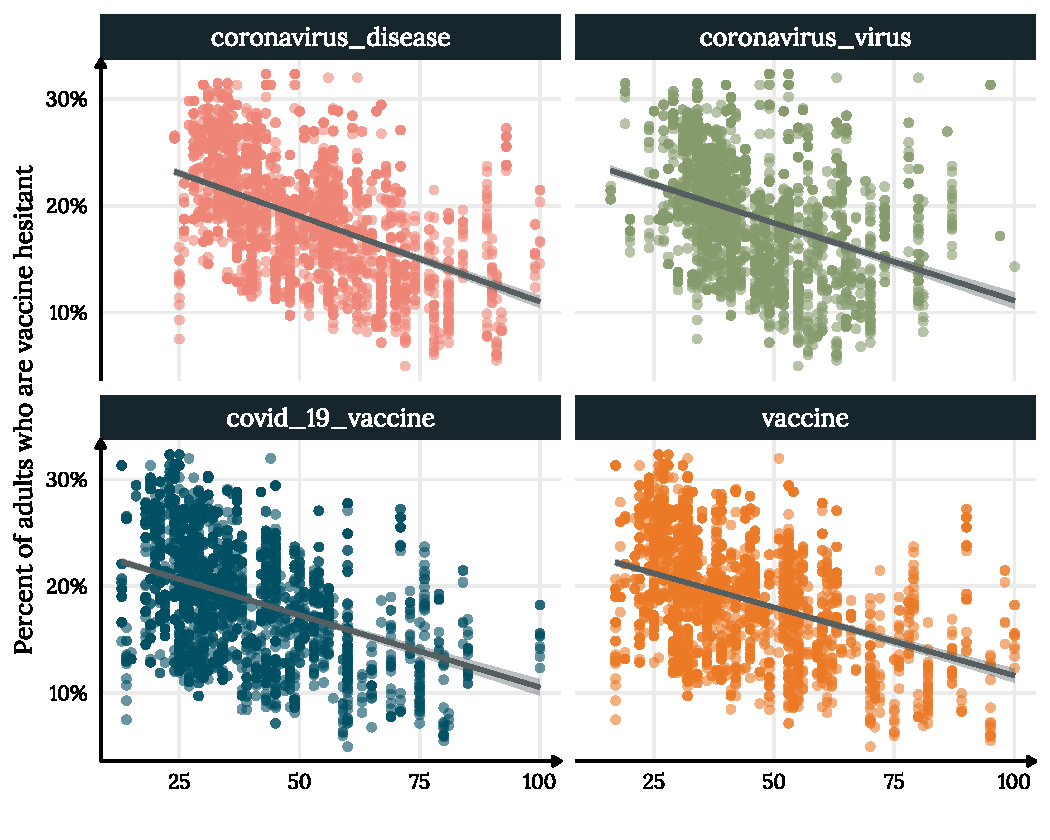
\includegraphics[width=0.8\linewidth]{figs/paper1/vacc_hes_plot-1.pdf}}
\caption{Vaccine hesitancy by each Google Trend with a fitted linear regression line}\label{fig:vacc_hes_plot}
\end{figure}


The second attitudinal measure I test is how Google Trends relates to rare mask
usage. As with vaccine hesitancy, the Pearson correlations are negligible.
Correlation's under |0.20| are negligible according to the
common standards. I introduce these trends in multiple linear regression in
table \ref{tab:mask_analysis}. Model 1 demonstrates that these five Google
Search Trends can explain about 8\% of the variance in mask usage across U.S.
counties, reinforcing the conclusion that the relationship is quite weak. The
coefficients themselves are significant in Model 1. However, after
including the demographic variables in Models 2 and 3, we see that the
relationship between the Google Search Trends and mask usage is strengthened in
magnitude and in significance, indicating a suppression effect due to
underlying relationships between the trends and demographic variables. While the
trends are significant and match the demographic variables in magnitude, the
low $r^2$ of 0.203 for the trends still provides evidence that Google Search
Trends data cannot replace survey analysis when trying to measure rare mask
usage.

\begin{table}[!h]

\caption{\label{tab:mask_analysis}Linear Regression Results for Rare Mask Usage}
\centering
\fontsize{8}{10}\selectfont

\begin{tabular}{lccc}
\toprule
  & Model 1 & Model 2 & Model 3\\
\midrule

Search for `Coronavirus Disease' & \num{-0.010}*** &  & \num{-0.012}***\\
 & (\num{0.003}) &  & \vphantom{1} (\num{0.003})\\
Search for `Coronavirus Virus' & \num{-0.012}*** &  & \num{-0.001}\\
 & (\num{0.003}) &  & (\num{0.003})\\
Search for `Cloth face mask' & \num{-0.009}* &  & \num{-0.015}***\\
 & (\num{0.004}) &  & (\num{0.004})\\
Search for `Mask' & \num{0.025}*** &  & \num{0.023}***\\
 & (\num{0.004}) &  & (\num{0.003})\\
Search for `Civil and political rights' & \num{-0.012}*** &  & \num{-0.008}***\\
 & (\num{0.002}) &  & (\num{0.002})\\
Total Population &  & \num{-0.012}*** & \num{-0.011}***\\
 &  & (\num{0.002}) & \vphantom{3} (\num{0.002})\\
Population Density &  & \num{-0.003}+ & \num{-0.004}*\\
 &  & (\num{0.002}) & \vphantom{2} (\num{0.002})\\
Unemployment Rate &  & \num{-0.028}*** & \num{-0.024}***\\
 &  & (\num{0.002}) & \vphantom{1} (\num{0.002})\\
\% over 65 &  & \num{-0.006}** & \num{-0.003}+\\
 &  & (\num{0.002}) & (\num{0.002})\\
\% below poverty line &  & \num{-0.010}** & \num{-0.009}**\\
 &  & (\num{0.003}) & \vphantom{2} (\num{0.003})\\
Median income &  & \num{-0.036}*** & \num{-0.030}***\\
 &  & (\num{0.003}) & \vphantom{1} (\num{0.003})\\
\% with broadband &  & \num{-0.006}* & \num{-0.007}**\\
 &  & (\num{0.003}) & (\num{0.003})\\
\midrule
Num.Obs. & \num{2964} & \num{3133} & \num{2954}\\
R2 & \num{0.077} & \num{0.176} & \num{0.203}\\
R2 Adj. & \num{0.076} & \num{0.174} & \num{0.200}\\
\bottomrule
\multicolumn{4}{l}{\rule{0pt}{1em}* p $<$ .05. ** p $<$ .01. *** p $<$ .001 (two-tailed test).}\\
\end{tabular}
\end{table}
\begin{figure}[h]
{\centering 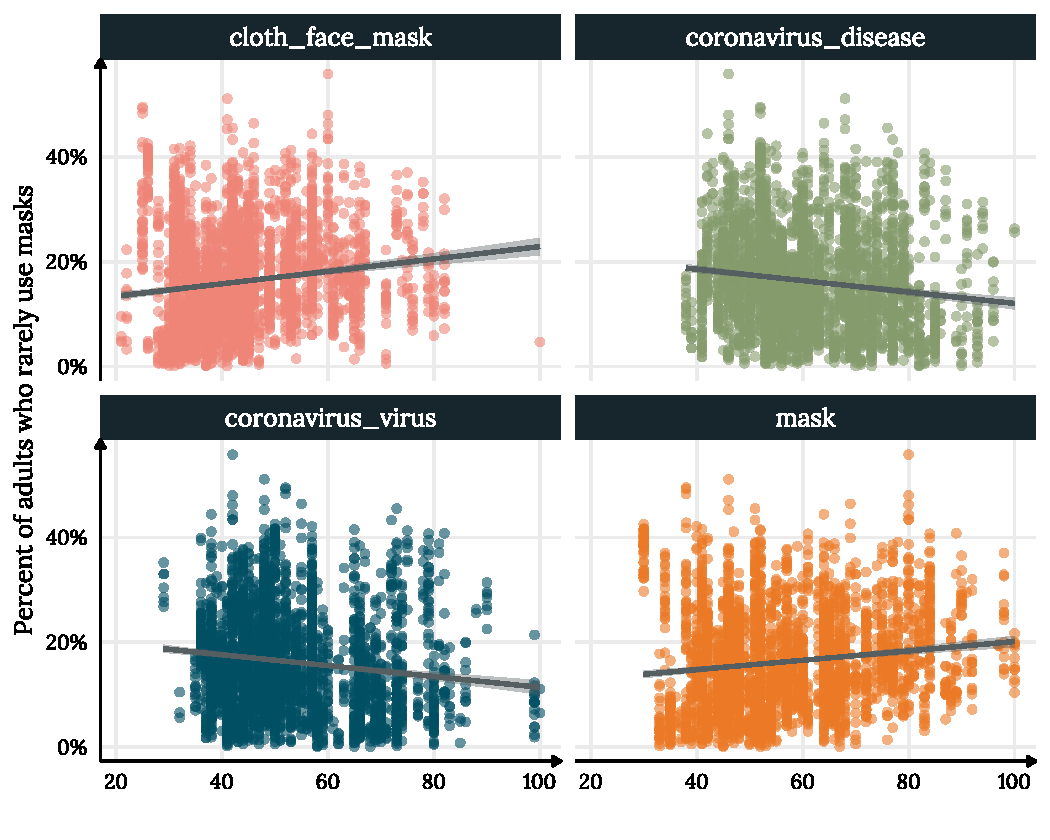
\includegraphics[width=0.8\linewidth]{figs/paper1/mask_plot-1.pdf}}
\caption{Rare mask usage by each Google Trend with a fitted linear regression line}\label{fig:mask_plot-1}
\end{figure}


\subsection{Validating Google Trends as metrics of health outcomes}

In addition to attitudinal measures, I attempt to validate Google Trends for
uses in the measurements of health indicators. The first indicator I assess is
COVID-19 case rates from 2020 through 2021. The Pearson correlation results
indicate negligible to weak relationships between the search terms and the
actual case rates across time and place. The repeated measures correlation
coefficient, a more reliable and less biased measure for longitudinal
correlations, reveals similarly weak results with a maximum correlation of 0.32
between 'smell loss' and rates of COVID-19. To further investigate the relationship, I
include the three trends in random intercept hierarchical linear models. Model 1
of Table \ref{tab:covid_analysis} indicates that the trends themselves are able
to explain about 20\% of the variation in COVID-19 rates ($r^2$ = 0.201). Few
of the demographic variables influence COVID-19 rates in models 2 or 3,
though there is some suppression for median income, unemployment rates,
and population density. Model 3 has an $r^2$ of 0.200. I conclude that the
Google Trends are slightly related to COVID-19 rates, but that this relationship
is weak, and we should not attempt to use Google Trends as an indicator of actual
health outcomes.

\begin{table}[!h]

\caption{\label{tab:covid_analysis}Hierarchical Model for Covid Case Rates}
\centering
\fontsize{8}{10}\selectfont

\begin{tabular}{lccc}
\toprule
  & Model 1 & Model 2 & Model 3\\
\midrule
covid\_19 & \num{1.031}*** &  & \num{1.024}***\\
 & (\num{0.082}) &  & \vphantom{1} (\num{0.082})\\
smell\_loss & \num{7.373}*** &  & \num{7.374}***\\
 & (\num{0.082}) &  & (\num{0.082})\\
taste\_loss & \num{6.344}*** &  & \num{6.347}***\\
 & (\num{0.078}) &  & (\num{0.078})\\
covid\_rate\_fips\_mean & \num{0.813}*** & \num{0.982}*** & \num{0.879}***\\
 & (\num{0.019}) & (\num{0.010}) & (\num{0.020})\\
date & \num{0.029}*** & \num{0.038}*** & \num{0.029}***\\
 & (\num{0.000}) & (\num{0.000}) & (\num{0.000})\\
total\_pop &  & \num{0.064} & \num{0.409}**\\
 &  & (\num{0.066}) & (\num{0.140})\\
pop\_density &  & \num{0.010} & \num{0.463}***\\
 &  & (\num{0.067}) & (\num{0.123})\\
unemployment\_rate &  & \num{0.049} & \num{0.725}***\\
 &  & (\num{0.080}) & (\num{0.155})\\
over\_65 &  & \num{-0.116} & \num{-0.055}\\
 &  & (\num{0.074}) & (\num{0.139})\\
poverty\_rate &  & \num{0.054} & \num{0.351}\\
 &  & (\num{0.118}) & (\num{0.221})\\
median\_income &  & \num{0.031} & \num{0.907}***\\
 &  & (\num{0.114}) & (\num{0.214})\\
broadband &  & \num{0.073} & \num{0.437}*\\
 &  & (\num{0.097}) & (\num{0.182})\\
\midrule
Num.Obs. & \num{248346} & \num{284666} & \num{247655}\\
R2 Marg. & \num{0.201} & \num{0.081} & \num{0.200}\\
R2 Cond. &  & \num{0.081} & \\
\bottomrule
\multicolumn{4}{l}{\rule{0pt}{1em}Random intercept per county}\\
\multicolumn{4}{l}{\rule{0pt}{1em}* p $<$ .05. ** p $<$ .01. *** p $<$ .001 (two-tailed test).}\\
\end{tabular}
\end{table}
\begin{figure}[h]
{\centering 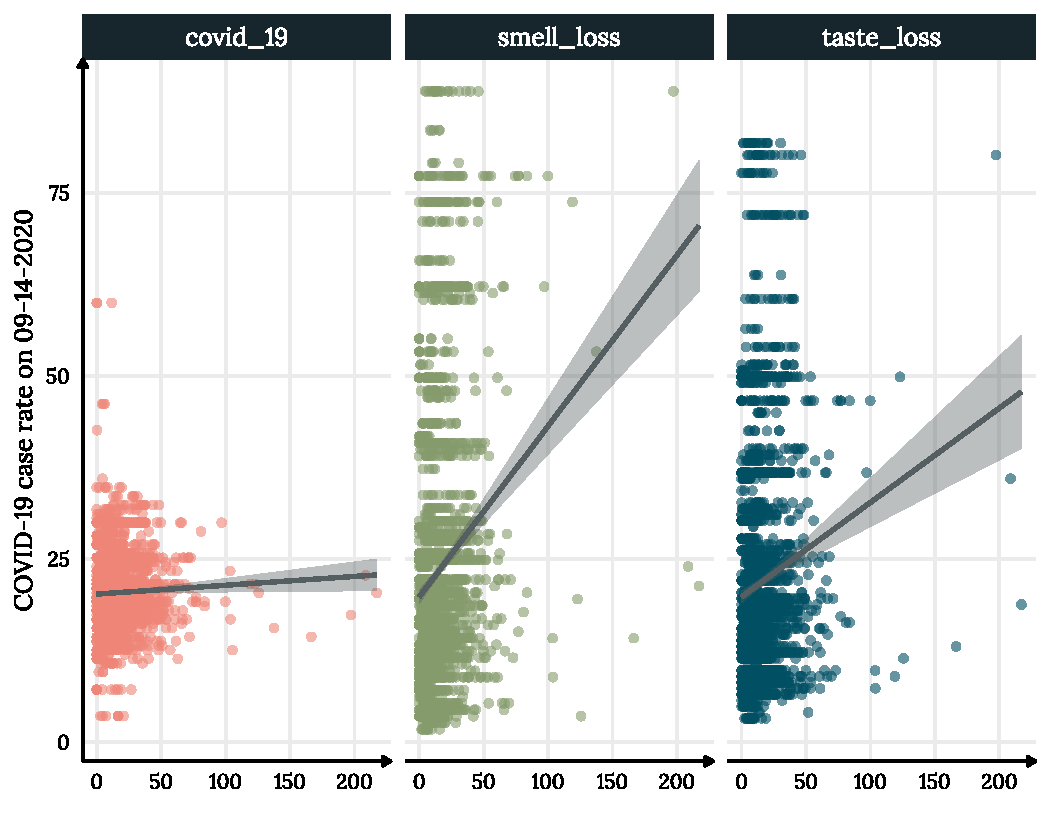
\includegraphics[width=0.8\linewidth]{figs/paper1/covid_plot-1.pdf}}
\caption{Covid case rate for 09-14-2020 by each Google Trend with a fitted linear regression line}\label{fig:covid_plot-1}
\end{figure}

Another health outcome I test is county suicide rates. As with previous cases,
there is only negligible correlation between actual suicide rates and Google
Search Trends, not exceeding 0.0845. In the more accurate repeated measures
correlation coefficient we see a maximum of 0.142 correlation, remaining
negligible. I introduce these trends into a random intercept model to control
for inter-group variation over time in Table \ref{tab:suicide_analysis}. While
table \ref{tab:suicide_analysis} model 1 reveals a statistically significant relationship
between suicide hotline trends and suicide rates, the effect is small, and the
entire model only has an $r^2$ of 0.058. Adding in demographic features in model
2 improves the $r^2$ to 0.56. In model 3, the inclusion of Google Trends
decreases the overall amount of suicide rate variance explained
compared to model 2. These analyses lead me to conclude that Google Search
Trends should not be used by researchers as indicators of suicide rates or intentions.

\begin{table}[!h]

\caption{\label{tab:suicide_analysis}Fixed Effect Model for Suicide Rates}
\centering
\fontsize{8}{10}\selectfont

\begin{tabular}{lccc}
\toprule
  & Model 1 & Model 2 & Model 3\\
\midrule

Search for `Suicide' & \num{-0.001} &  & \num{-0.001}\\
 & (\num{0.001}) &  & \vphantom{2} (\num{0.001})\\
Search for `Depression' & \num{-0.001}+ &  & \num{-0.001}\\
 & (\num{0.001}) &  & \vphantom{1} (\num{0.001})\\
Search for `Suicide Hotline' & \num{0.002}*** &  & \num{0.002}***\\
 & (\num{0.001}) &  & (\num{0.001})\\
Year & \num{0.004}*** & \num{0.005}*** & \num{0.005}***\\
 & (\num{0.000}) & (\num{0.000}) & (\num{0.000})\\
Total Population &  & \num{-0.032}*** & \num{-0.027}**\\
 &  & (\num{0.010}) & (\num{0.009})\\
Population Density &  & \num{-0.037}** & \num{-0.033}**\\
 &  & (\num{0.011}) & (\num{0.011})\\
Unemployment Rate &  & \num{-0.001} & \num{-0.001}\\
 &  & (\num{0.001}) & \vphantom{1} (\num{0.001})\\
\% over 65 &  & \num{-0.010}*** & \num{-0.014}***\\
 &  & (\num{0.002}) & \vphantom{1} (\num{0.002})\\
\% below poverty line &  & \num{-0.005}*** & \num{-0.003}**\\
 &  & (\num{0.001}) & (\num{0.001})\\
Median income &  & \num{-0.014}*** & \num{-0.015}***\\
 &  & (\num{0.002}) & (\num{0.002})\\
\midrule
Num.Obs. & \num{30008} & \num{33582} & \num{30001}\\
R2 Marg. & \num{0.058} & \num{0.582} & \num{0.564}\\
\bottomrule
\multicolumn{4}{l}{\rule{0pt}{1em}Fixed intercept per county}\\
\multicolumn{4}{l}{\rule{0pt}{1em}* p $<$ .05. ** p $<$ .01. *** p $<$ .001 (two-tailed test).}\\
\end{tabular}
\end{table}
\begin{figure}[h]
{\centering 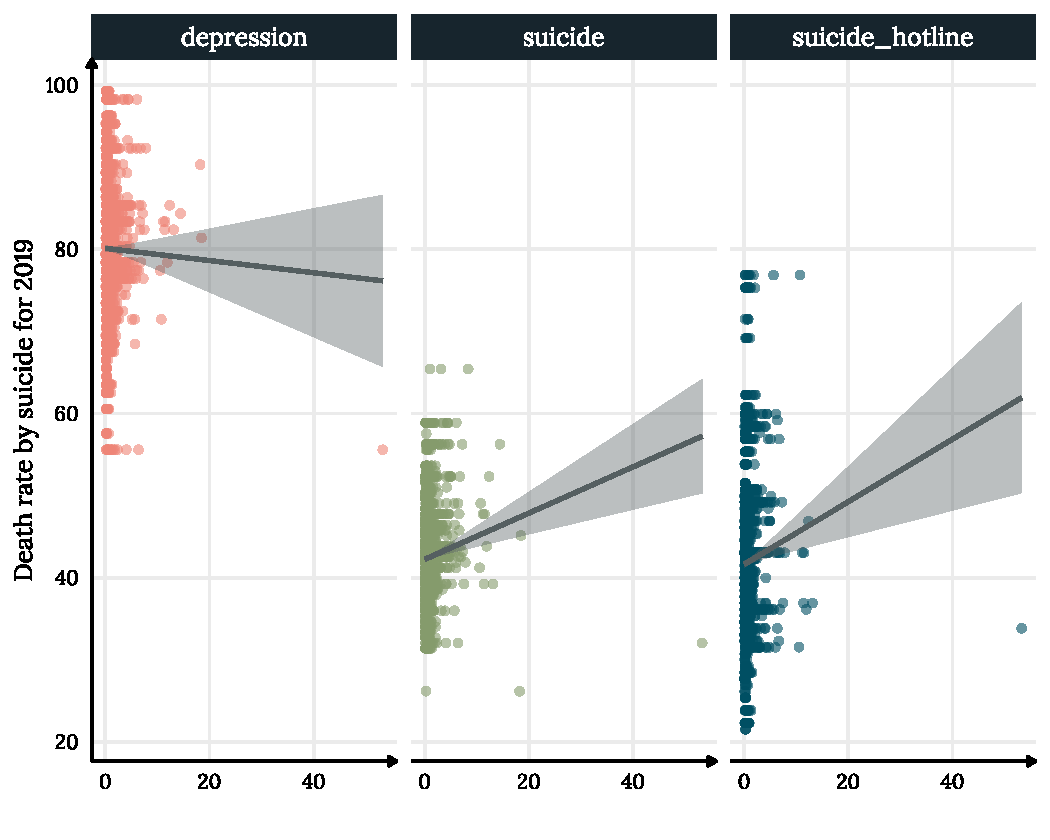
\includegraphics[width=0.8\linewidth]{figs/paper1/suicide_plot-1.pdf}}
\caption{Suicide death rate for 2019 by each Google Trend with a fitted linear regression line}\label{fig:suicide_plot-1}
\end{figure}

\subsection{Validating Google Trends as metrics of political support}

Previous research has shown some relationship between Google Search Trends and
political election results. I investigate the relationships between search trends
and U.S. Presidential Election results in 2016 and 2020. In 2016, Pearson
correlations for Both Hilary Clinton and Donald Trump do not exceed a |0.17|
correlation with the actual percentage of votes for either candidate. In 2020,
results are even less related, with searches for neither Joe Biden nor Donald
Trump holding any real correlation with the 2020 results.

In Table \ref{tab:pres_2016_analysis}, I outline the results for the model
predicting the county percentage of votes for Hillary Clinton. Model 1
demonstrates how well Google Trends predict the votes; while the
trend for 'Hillary Clinton' is significantly associated with votes, the model's
$r^2$ ($r^2$ = 0.027) shows that it does little to help explain the model
variance. On the other hand, adding in demographic features improves the model
fit quite well, bringing the $r^2$ up to 0.313 in model 2 and $r^2$ 0.327 in
model 3. Table \ref{tab:pres_2020_analysis} shows this same analysis for the
2020 election and predicts the percentage of votes for Joe Biden. While this
model is analogous to those in Table \ref{tab:pres_2016_analysis}, this
model 1 demonstrates how unrelated Google Trends can be from actual outcomes. In
conclusion, I find that Google Trends are an unreliable and invalid indicator of
political support.

\begin{figure}[h]
{\centering 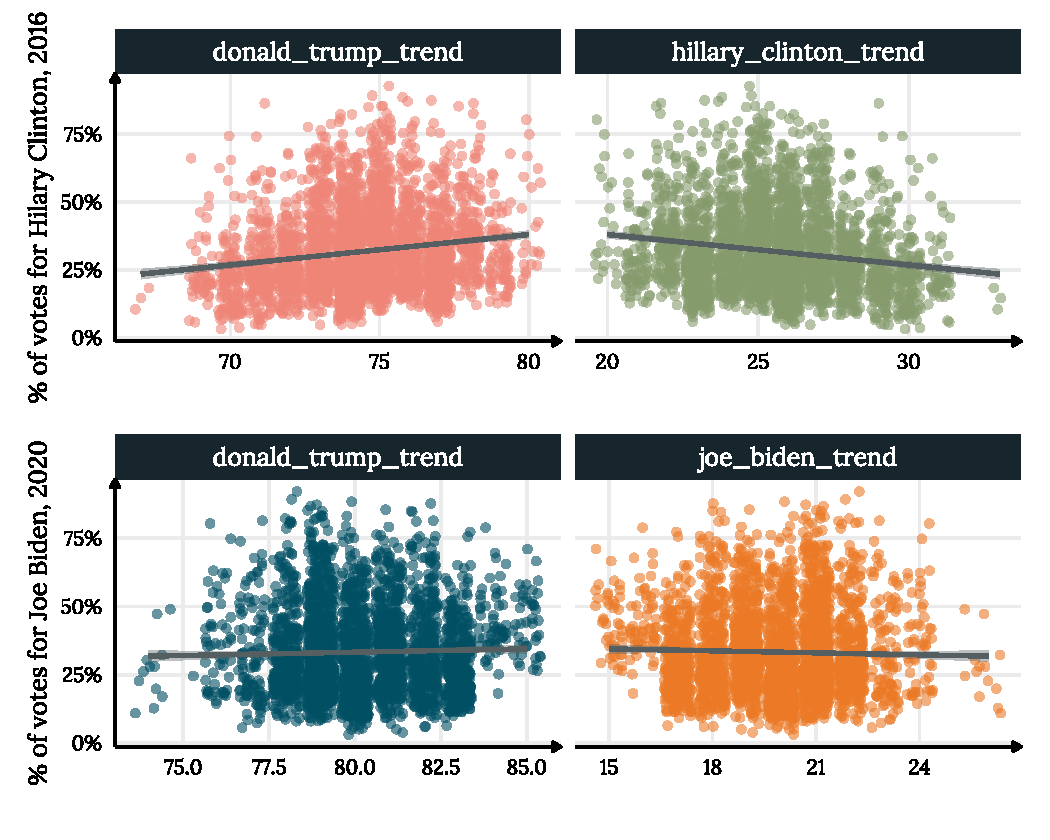
\includegraphics[width=0.8\linewidth]{figs/paper1/pres_plot-1.pdf}}
\caption{Presidential voting outcomes for 2016 and 2020 by each Google Trend with a fitted linear regression line}\label{fig:pres_plot-1}
\end{figure}

\begin{table}[!h]
\caption{\label{tab:pres_2016_analysis}}
\centering
\begin{tabular}[t]{}
\end{tabular}
\end{table}
\begin{table}[!h]

\caption{\label{tab:pres_2020_analysis}Linear Regression Results for 2020 Presidential Election Results (Joe Biden Shown)}
\centering
\fontsize{8}{10}\selectfont

\begin{tabular}{lccc}
\toprule
  & Model 1 & Model 2 & Model 3\\
\midrule

Search for `Joe Biden' & \num{-0.005} &  & \num{-0.014}***\\
 & (\num{0.003}) &  & (\num{0.002})\\
Total Population &  & \num{0.030}*** & \num{0.029}***\\
 &  & (\num{0.003}) & \vphantom{3} (\num{0.003})\\
Population Density &  & \num{0.021}*** & \num{0.022}***\\
 &  & (\num{0.003}) & \vphantom{2} (\num{0.003})\\
Unemployment Rate &  & \num{0.044}*** & \num{0.044}***\\
 &  & (\num{0.003}) & \vphantom{1} (\num{0.003})\\
\% over 65 &  & \num{-0.007}* & \num{-0.008}**\\
 &  & (\num{0.003}) & (\num{0.003})\\
\% below poverty line &  & \num{0.032}*** & \num{0.033}***\\
 &  & (\num{0.004}) & \vphantom{1} (\num{0.004})\\
Median income &  & \num{0.069}*** & \num{0.070}***\\
 &  & (\num{0.004}) & (\num{0.004})\\
\midrule
Num.Obs. & \num{3118} & \num{3118} & \num{3118}\\
R2 & \num{0.001} & \num{0.295} & \num{0.303}\\
R2 Adj. & \num{0.000} & \num{0.294} & \num{0.301}\\
\bottomrule
\multicolumn{4}{l}{\rule{0pt}{1em}Results predicting Donald J. Trump comparable and available upon request.}\\
\multicolumn{4}{l}{\rule{0pt}{1em}* p $<$ .05. ** p $<$ .01. *** p $<$ .001 (two-tailed test).}\\
\end{tabular}
\end{table}

\section{Discussion and Conclusion}
%TODO I’d say it is a test or assessment. Critique implies the answer is known a priori. I would focus on validation, note it it has implication (we need to test more and be more cautious),  and say future research should x,y,z. 

% The critique, is really about how and why we overlook being precisely incorrect if we like the aesthetics of an argument. I can think of some egregious examples.

% I would send the first paper to somewhere like soc methods or a stat journal, and the second to big data and society or the like.

% That said, there are things here that die hard stats people may find issues with. I also think a direct comparison of what google trends versus traditional survey data would predict would be very strong evidence of literally missing the mark.

% A related thought, is the assumption is the survey is right, since it is the referrant for validation. But often, the validation procedures of surveys can also lead to invalid claims. Cicourel wrote about this really well in 1982, and there are examples where a measure means totally different things to different respondents. E..g Alcohol may be read as ‘spiritis’ but not wine by some groups. So, it is possible that google is more accurate, and all these data sources require validation from interactions with humans in their lifeworld. That would be my position at least, but I think it is fair to say that the while the surveys have been more thoroughly tested, there are potential errors there as well.


This paper provides a test of the criterion validity of Google Trends for use in Social Science. 
I failed to find correlation between the Google Trends and their 
validated indicators. While some Google Trends tested were significantly 
associated with the outcome in the linear regression model, effects tended
to be small and the total model interpretability remained low, even when 
controlling for demographic variables.  

Some previous research has shown strong innovation in the computational social sciences
to gather sociodemographic data when survey or other research methods are too costly
\citep{blumenstockPredictingPovertyWealth2015}. Google Trends, in theory, sounds like 
a promising data source to 'nowcast' attitudinal, health, and political indicators.
Not only would the data be easily and freely accessible, but it would also provide 
indicators for areas where conducting research may be too costly. The demand for this 
sort of indicator is clear and fields like the health sciences have freely utilized
this data source. However, this article shows that Google Trends
fails to map on to validated survey metrics for attitudes, disease prevalence and political preferences.
Social scientists should not assume Google Trends data can serve as a replacement
for high quality survey data, at least for these measures. 

As social scientists it is our responsibility to deeply investigate the validity 
of the data that we use so we can be confident in our research findings. As with any
source of data, we must consider the potential pitfalls, especially in research on 
using new methods and data sources \citep{mcfarlandBigDataDanger2015}.
In the case of Google Search Trends, precaution is warranted.
\newpage
\section{References}
\begin{singlespace}
\printbibliography[heading=none] % print section bibliography
\end{singlespace}
\end{refsection}


\begin{refsection} % refsection environment
\hypertarget{paper-2}{\chapter{Information seeking Behaviors for Information on COVID-19 Vaccinations}\label{paper-2}}

\hypertarget{abstract}{\section{Abstract}\label{abstract}}

Previous research has greatly failed to distinguish between the activation of
information seeking behaviors online and offline. Using theories of 1) social
support and 2) uses and gratifications theory I investigate the factors
associated with each type of information search: 
personal connection, doctor, social networking site, online forum, and online
search engine. Using novel survey data of 948 Americans and their experience
seeking out information about the COVID-19 vaccines, I find little evidence that
online search is more utilized than seeking social support from personal network
connections or health professionals. I find evidence that the modalities queried
in this survey are conceptually different and that the utilization of different
modalities varies by demography and information exposure points, where
individuals are provided with information without seeking it. Finally, I find that
different sources of information exposure and information search modalities hold
real world consequences through their associations with COVID-19 vaccination
intentions and rates, as information from a doctor increases COVID-19
vaccination uptake while receiving information from a social networking site
is associated with lower odds of vaccination.

\textbf{Keywords}: information seeking Behavior, COVID-19, Vaccine Hesitancy, Social Networks, Social Support, Information \& Communication Technologies

\hypertarget{intro-1}{\section{Introduction}\label{intro-1}}

Information is all around us and permeates every facet of human society, from
the hordes of data gathered during the internet age to passing gossip between
friends. Human communication and human society are based on the circulation of
information and knowledge. Information can be shared by others through
information campaigns and consumed by an individual, called information push, or
intentionally sought out by individuals, called information pull
\citep{cybenkoFoundationsInformationPush1999}.

Information push and pull are inherently tied to arguments of structure and agency.
That is, to what extent does the structure and institutions of society shape 
individual human behavior and to what extent do individuals actors control 
the decisions they make in the environment in which they find themselves. 
Attempts to reconcile the false dichotomy between structure and agency
are found among the majority of modern sociological theorists, particularly  
\citet{coleman1994foundations} and \citet{bourdieu1987distinction}.
Both renowned sociologists theorize how the external structures
are internalized by actors and inspire individual agency, which in turn 
can lead to an evolution of the external structures themselves.  
This article joins Coleman and Bourdieu in rejecting the false dichotomy
between structure and agency by investigating the complementary push (structure)  
and pull (agency) of information diffusion.

Information is especially important given the prominent trends of
misinformation, disinformation, and mistrust in traditional institutions
\citep{starbird19, kata10}. While no belief in false information can be thought
of as harmless \citep{douglas21} some discredited theories such as `vaccines
cause autism' have major ramifications for both the individual and public
health. For example, a newfound public resistance to vaccination against Measles
by so-called `anti-vaxxers' caused a 17\% increase in rates worldwide in 2019.
This increase killed  142,000 people, most of whom were children under the age
of five \citep{givetash19}. However, even in the ever-evolving research agenda
of misinformation and infodemiology \citep{eysenbach02}, much of the research
focuses on the `push' or `supply' side of information, like spaces where
individuals first encounter conspiracy theories or other information
\citep{johnsonOnlineCompetitionPro2020, broniatowski_etal20}.

The lack of research in which modalities are likely to be chosen when an
individual faces a need for information makes it difficult for policy makers to
propose effective information campaigns that promote the health and well-being
of individuals in our society. Even outside of the misinformation literature,
much of the research conducted in social networks and communication focus on
senders, influencers, and persuasion strategies
\citep{mertonManifestLatentFunctions1968, katzPersonalInfluencePart1955,
lazarsfeldPeopleChoice1944}, rather than on ``the receiver as an active
information seeker and processor''
\citep[][p. 344]{johnsonComprehensiveModelCancerRelated1993} \citep[for an exception,
see][]{eysenbach09}.

I use the case of information around COVID-19 vaccinations to explore the
variation of usage of information search modalities. In doing so, I seek to
answer how computer-mediated or interpersonal information seeking strategies
vary across populations as people search for information about COVID-19
vaccinations, and I investigate how these strategies affect vaccination uptake.
Specifically, this article answers two research questions: (1) How do
computer-mediated or interpersonal information seeking strategies vary across
populations? (2) How does the information search modality utilized affect
COVID-19 Vaccination uptake?

Before addressing the results to these research questions, I offer an overview
of the current state of social science literature in regards to information
seeking strategies and provide a description of the research methodology and
analytic sample. I then discuss the implications of these findings for the
sociological understanding of information search and vaccination uptake.

\hypertarget{information-search}{\subsection{Information Search}\label{information-search}}

Active, directed searching by individuals to obtain information is sparsely
discussed in the sociological literature.
\citet{pejtersenDesignComputeraidedUsersystem1984}, a scholar of library and
information science, theorized that there are five strategies for searching for
information: browsing, analytical, empirical, known site, and similarity. The
most common strategy is browsing, where people follow leads based on
associations without premeditation. Another strategy is analytical, which
includes an explicit consideration of all facets of the question to guide a
search. The empirical method guides the search based on tactics that were
successful in past research. The known site strategy is to go to the direct
source of the information if known. And finally, the similarity method is to
find information based on another similar question that already has an answer.
These five strategies vary in their demands for prior knowledge, cognitive
processing, memory, and time spent. While this theory is aimed at finding
information in a library setting, scholars have extended the theory to other
fields and validated the framework \citep{fidelHumanInformationInteraction2012};
the frame is a useful beginning point for my theories of information search
through network activation or through computer-mediated communication.

Some communication theorists ask why an answer to a question is sought in the
first place. The Theory of Uncertainty Management
\citep{brashersCommunicationUncertaintyManagement2001} professes that people
search for information when their uncertainty around the subject leads to
anxiety or other cognitive harms. The Theory of Motivated Information Management
\citep{afifiTheoryMotivatedInformation2004, afifiSeekingInformationSexual2006}
extends the prior by adding that uncertainty itself is not the catalyst for
information-search; rather, it is driven by a discrepancy between the current
level of uncertainty on a subject and desired level of uncertainty. In other
words, individuals only perform information search when they are distressed by
their lack of knowledge or understanding on a subject.

One way to find information is to activate network ties to secure information
through a form of social support. Social support, while previously used
interchangeably with the terms social networks and social integration
\citep{houseStructuresProcessesSocial1988}, are the emotional, informational,
and instrumental assistance functions performed between social ties and have
strong and measurable association with health outcomes
\citep{houseMeasuresConceptsSocial1985, thoitsMechanismsLinkingSocial2011}.
Informational support is the process of seeking ``help in defining,
understanding, and coping with problematic events and include education, advice,
or referral to another source of support'' \citep[][p. 640]{winemiller_etal93}.
Brashers, a health communications researcher, defines informational support
slightly differently, focusing on the exchange of information that ``facilitates
coping with life stresses… that may be exchanged among members of a support
network'' \citet[][p. 260]{brashersInformationSeekingAvoiding2002}. These
definitions help to differentiate between seeking information through social
ties or through something anonymous like online search; a need for coping or
deeper understanding of important matters is thought to sway that decision.

Social support has long been theorized to stem from core discussion networks and
much of the historical social support surveys only examined these core networks.
The underlying assumption is that individuals reach out to a handful of strong
ties when in need of support, which could be elicited in surveys using name
generators \citep{marsdenCoreDiscussionNetworks1987}. This approach has yielded
important insights, but largely overlooks crucial processes of resource
activation \citep{hurlbertCoreNetworksTie2000, perrySocialNetworkActivation2015,
smithDonPutMy2005}. For instance, \citet{smallSomeoneTalk2017} shows that
the core discussion network does not capture how people activate social support
in practice and indicates that people draw on much broader social connections
for support, reminiscent of the weak ties research by \citet{granovetterStrengthWeakTies1973}.
There is ongoing research investigating
how weak-tie support holds for different support types based on the architecture
put forward by \citet{houseStructuresProcessesSocial1988} of instrumental,
emotional, and informational support.

However, informational support can also be sought outside of the social network
context, namely via computer-mediated information search tools such as the
process of ``Googling'', or the utilization of internet search engines. As the
online environment began penetrating all facets of modern human life, it makes
sense that performing online search has become one of the most convenient
modalities for information search. \citet{smallSomeoneTalk2017} showed
that graduate students often confided in ``miscellaneous classmates encountered
down the hall'' (p. 176) instead of established and trusted confidants because
they simply were there at the right time. 
% Ron: Is it that simple? I think you have a lot in common with ``misc classmates down the hall'' in comparison with, let's say, a random sample of same-aged Tucsonans.
I theorize that online search engines
may be the most frictionless and costless mode of support. No social capital or
relationship is necessary when choosing to utilize a search engine. 

There are three computer-mediated modalities I consider for this analysis: online
search engines like Google or Bing, posting questions on online forums like
subreddits or Facebook groups, and posting a status update online via Facebook
or Twitter. While the first two are largely anonymous and do not require a
personal network, the third is a unique hybrid between personal network
connections and online search.

There are important factors that can influence information seeking strategies
besides the strength of social capital or ease of search. For instance, we can
borrow uses and gratifications theory (UGT) from studies of mass communication
\citep{blumlerUsesMassCommunications1974, tanMassCommunicationTheories1985}. UGT
posits that users are not passive consumers of media and that people have an
active role in choosing different sources of media based on their satisfaction
of specific needs on an individual basis. UGT is based on Maslow’s
\citeyear{maslowTheoryHumanMotivation1943} hierarchy of needs.
Modern-day theorists have extended UGT theory
and classified the uses and gratifications of the internet and of social media.
\citet{staffordDeterminingUsesGratifications2004} theorize that the internet
provides gratification through useful content that meets expectations,
gratification from purposeful navigating or random browsing as a process, and
social gratification from forming and deepening social ties.
\citet{leungGenerationalDifferencesContent2013} theorizes that social media is
gratifying for users because it allows for venting of negative feelings,
provides recognition, provides entertainment, promotes social affection, and
fulfills cognitive needs.

Adapting these facets of UGT and social support to my own case, I theorize that
online search allows for increased anonymity, a lowered social cost, and the
potential avoidance of embarrassment and other negative social interactions,
especially in the case on search engines.

\begin{hyp}[H\ref{hyp:online-vs-network}] \label{hyp:online-vs-network}
The proportion of survey respondents who seek information
using an online search engine will be significantly higher than those who
need to activate network resources, like asking a friend.
\end{hyp}

% this actually makes more sense not from UGT but as a transactional cost perspective (maybe like disposable ties), that you have to use social capital to activate your social network, but online search is free. 

\citet{rainsCopingIllnessDigitally2018} finds that while patients tend to search for
technical information about an illness online, they then turn to their social
network for experiential information from others facing similar circumstances in
the case of cancer. The type of information sought is therefore important. If
specific expertise on a specific topic is desired by a searcher, they may reach
out to personal connections that they see as expert such as a doctor. Or, if an
individual distrusts the medical establishment, they may be more likely to
activate informational support among their social network or turn to online
groups that validate their worldview \citep{bogersHowSocialAre2014}. Finally,
UGT and Brasher's definition of social support
\citeyearpar{brashersInformationSeekingAvoiding2002} help us to theorize that
psychosocial needs like identity management or relational maintenance of each
individual may influence their chosen information search modality: when the
informational need is related to forming and deepening social ties search is
likely to be done from network ties.

\begin{hyp}[H\ref{hyp:drgooglefriend}] \label{hyp:drgooglefriend}
Seeking information from experts, search engines, and other people
will each be significantly more utilized modes of information search than seeking via 
online forums and social networking sites. 
\end{hyp}

\hypertarget{research-methodology}{\section{Research Methodology}\label{research-methodology}}

The data used for this research project are based on original survey data
collected between December 03, 2021 through December 12, 2021. This survey was
hosted on Qualtrics and participants were paid and recruited using Amazon Turk
(MTurk). Potential MTurkers were invited to participate if they were located in
the United States, had a task rate approval of over 95 percent, had completed 50
tasks, and had not completed this survey in previous sessions. The total valid
survey responses (\emph{n} = 948) were selected from a total of 1,066
respondents; some responses were disqualified due to a few factors such as
detected usage of a VPN, random answer clicking (determined by illogical
responses), poor quality typed responses (e.g.\, social network alters
consistently named random nouns), or taking the survey more than once. The
sample is slightly gender unbalanced, skewing towards male respondents. For the
respondents who provided their zip code (p = 0.98), the sample is quite balanced
with a slight skew towards MTurkers in the South (p = 0.41).

The survey took an average of 24.48 minutes with a standard deviation of 13.23
minutes. The shortest valid survey took 3.75 minutes and the longest took 111.08
minutes. Participants received \$6.00 in compensation for their participation in
the survey \footnote{All funding for this survey was provided by a Grant from
the Summer Institute in Computational Social Science and the Russell Sage
Foundation.}. The survey consisted of two main parts. The first portion of the
survey is a replication of they survey conducted by
\citet{smallSomeoneTalk2017}. In this section, I expand Small's research on
support activation by segregating weak-tie social support into instrumental,
emotional, and informational categories
\citep[see][]{houseStructuresProcessesSocial1988}. The second part of the survey
focuses on network resource activation and information seeking behaviors of
individuals regarding COVID-19 vaccinations for this paper.

\begin{table}[!ht]

\caption{\label{tab:table-1-ind}Descriptive Statistics for Dependent Variables}
\centering
\begin{tabular}{llrrr}
\toprule
  &    & Mean & SD & 95\% CI\\ \midrule
Sought Info & Overall  &  \num{0.78} & \num{0.41} & \num{0.76} to \num{0.81}\\
Sought Info & Doctor & \num{0.44} & \num{0.50} & \num{0.41} to \num{0.47}\\
Sought Info & Person & \num{0.42} & \num{0.49} & \num{0.39} to \num{0.45}\\
Sought Info & Online Search & \num{0.41} & \num{0.49} & \num{0.38} to \num{0.45}\\
Sought Info & Online Forum & \num{0.27} & \num{0.44} & \num{0.24} to \num{0.30}\\
Sought Info & Social Networking Site & \num{0.18} & \num{0.39} & \num{0.16} to \num{0.21}\\
\bottomrule
\multicolumn{5}{l}{\rule{0pt}{1em}Notes: 948 Surveyed, Conducted December 03 through December 12, 2021.}\\
\end{tabular}
\end{table}

\hypertarget{measures}{\subsection{Measures}\label{measures}}

\hypertarget{sought-information}{\subsubsection{Sought Information}\label{sought-information}}

There are multiple dependent variables of interest for this paper. The first
variable is a dichotomous indicator of whether someone intentionally sought out
information about COVID-19 vaccinations. The survey asked, ``And how about you
yourself intentionally looking for information about a COVID-19 vaccine? Such
information can include things such as advice, clarification, facts, and
experiences.'' About 78\% (\(\widehat{p}\))
of respondents had intentionally sought out information about COVID-19
vaccinations (95\% Confidence Interval = \{76\%, 81\%\}).

Further dependent variables segment the above question into multiple options;
``How did you look for information about the COVID-19 vaccine?'' Respondents
were posed with 5 responses and `other,' of which they could select multiple.
The largest proportion, 44\%, asked their `doctor or another health
professional'. About 42\% said they asked, `a person like friend, neighbor, or
family member that [they] know'. An additional 41\% searched `for [their]
question using an online search engine such as Google or Bing'. About a quarter
of the sample, 27\%, `posted queries in an online discussion group, listserv, or
other online forum like a Facebook Group or Subreddit'. And finally, 18\% of the
sample `posted queries on a social networking site such as Facebook timeline,
Twitter status update, or LinkedIn'. Much of the question wording and the
specific categories of search were inspired by ICPSR project 37220
\citep{scanlon19}. While each survey is not a direct comparison to the other, \citet{scanlon19}'s 
research focused on patient activation and health care utilization 
and therefore provided relevant, already validated survey questions for this survey.

\hypertarget{vaccination-outlook}{\subsubsection{Vaccination Outlook}\label{vaccination-outlook}}

Another dependent variable for this analysis is a dichotomous variable
indicating whether the respondent has received or plans to receive a vaccination
against COVID-19. For this survey, the number of doses or timeline of receipt
were less relevant to the research question. This variable instead focuses on
intent or opinion about the vaccine. About 87\% have a positive view about the
vaccine. This construct is made through the combination of two survey items. The
first item is actual vaccination status, obtained through the question `Did you
receive a COVID-19 vaccine?' 84\% of the sample said that they had indeed
received a vaccination (95\% Confidence Interval = \{82\%, 87\%\}). As the
national vaccination rate is closer to 75\% \citep{cdc20}, this indicates some
bias in our sample that must be acknowledged: either MTurkers are more likely to
be vaccinated than the normal population (sampling bias) or there is some
conformity bias in the responses causing survey takers to provide false answers.
The second survey item that contributes to `Vaccination Outlook' was only given
to those who had not responded `yes' to their vaccination status. These
respondents were asked `Do you plan to receive a vaccine for the prevention of
the COVID-19 virus?' Of those who were asked this question (n = 147), 9\% said
they were `definitely yes' getting the vaccine; 9\% said they were `probably
yes' going to receive vaccine. The rest of the sample was more unsure: 15\% said
they `Might or might not,' 26\% said `Probably not,' and finally 41\% said they
would `definitely not' receive the vaccine. The variable `Vaccination Outlook'
indicates that either the respondent received a COVID-19 vaccine or either
probably or definitely will in the future.


\begin{table}[!ht]

\caption{\label{tab:table-2-dep}Descriptive Statistics for Independent Variables}
\centering
\fontsize{10}{12}\selectfont
\begin{tabular}{llrr}
\toprule
\multicolumn{2}{l}{Numeric \& Dichotomous Variables} & Mean & SD\\
\midrule
Received info & From any source & \num{0.66} & \num{0.47}\\
Received info & Doctor & \num{0.47} & \num{0.50}\\
Received info & Person & \num{0.67} & \num{0.47}\\
Received info & News & \num{0.65} & \num{0.48}\\
Received info & Social Networking Site & \num{0.40} & \num{0.49}\\
Received info & Online Forum & \num{0.35} & \num{0.48}\\
Vaccination Status &  &  \num{0.84} & \num{0.36}\\
Vaccination Outlook &  &  \num{0.87} & \num{0.34}\\
Age &  & \num{37.76} & \num{10.75}\\
Hispanic or Latino/x &  & \num{0.15} & \num{0.36}\\
Race & White & \num{0.88} & \num{0.33}\\
Race & Black & \num{0.08} & \num{0.27}\\
Race & Native American & \num{0.03} & \num{0.16}\\
Race & Asian or Pacific Islander & \num{0.04} & \num{0.20}\\
Associate's Deg or above &  & \num{0.74} & \num{0.44}\\\toprule
\multicolumn{2}{l}{Categorical Variables}  &  N & Percent\\\midrule
Gender & Female & 418 & \num{44.09}\\
 & Male & 524 & \num{55.27}\\
 & Other & 6 & \num{0.63}\\
Plan to be Vaccinated, if not & Probably not & 38 & \num{4.01}\\
 & Definitely yes & 13 & \num{1.37}\\
 & Definitely not & 61 & \num{6.43}\\
 & Might or might not & 22 & \num{2.32}\\
 & Probably yes & 13 & \num{1.37}\\
\bottomrule
\multicolumn{3}{l}{\rule{0pt}{1em}Notes: 948 Surveyed, Conducted December 03 through December 12, 2021.}\\
\end{tabular}
\end{table}

\hypertarget{independent-variables}{\subsubsection{Independent Variables}\label{independent-variables}}

The first independent variables used in this analysis are based on the question,
`In the past 12 months, without searching for it, did you receive information
about the COVID-19 vaccine from \ldots{} (check all sources you received
information from).' This differs from the `How did you look for information'
question above because this is based on passive reception of information. The
largest proportion of respondents had received information from ``a person like
friend, neighbor, or family member that [they] know'' (\(\widehat{p}\) = 67\%).
Respondents also commonly received information from a television news channel or
a newspaper, about 65\% of the sample. 47\% of the sample had received
information from their doctor or other health professional, while 40\% received
information from a social networking site such as Facebook timeline, Twitter
status update, or LinkedIn. Finally, the lowest proportion of the sample had
received information from an online discussion group, listserv, or other online
forum like a Facebook group or subreddit (\(\widehat{p}\) = 35\%).

We also asked various demographic questions to describe our sample. The average
age of our sample was 37.76. 44\% of our sample self-identified as female, while
55\% self-identified as male. The sample is diverse racially though some ethnic
groups are underrepresented compared to national averages. Race was evaluated
using the question, `What is your race? If you are ``mixed race,'' select all
that apply.' Because of the multi-selection question, each variable is
dichotomous and proportions are shown. 88\% of the sample claimed they were
`White,' 8\% claimed to be `Black or African American,' 3\% chose `American
Indian or Alaskan Native,' 4\% selected `Asian,' and finally when asked, `Are
you Hispanic, Latino/a/x, or Latin American Origin?' 15\% selected `Yes.'
Respondents were also asked to select the highest level of education that you
have completed. Based on the breakdown between `Less than high school,' `High
school graduate,' `Some college,' `Associate's or Technical degree,' `Bachelor's
degree,' and `Graduate or professional degree,' 74\% of the sample were
classified to have a college-level education (Associate's degree or above).

\hypertarget{analysis}{\section{Analysis}\label{analysis}}

My analytic strategy proceeds in four steps. In Tables \ref{tab:table-1-ind} \&
\ref{tab:table-2-dep}, I present descriptive statistics for all study variables,
including variable ranges, means, and standard deviations. For this paper, I
rely heavily on logistic regression, modeled in \texttt{r}; specifically, I fit
a series of binomial generalized linear models with a logit link
\citep{venables2002a}, otherwise known as logistic regression model
\citep{hothorn2006handbook}. This approach is appropriate because the data are
non-nested, cross-sectional data with binary independent variables. In Table
\ref{tab:table-model-1}\footnote{All Tables in this paper were created with the
modelsummary package in \texttt{r} \citep{modelsummary}}, I fit a logistic
regression model predicting whether someone sought information about COVID-19
using their sources of information (`Received info') as well as various
demographic variables such as age, education level and race. Figure
\ref{fig:plot-model-1} then illustrates the relationship between the
coefficients and information seeking.\footnote{Figures in this paper were all
created using the \texttt{r} packages jtools \citep{jtools} and ggplot2
\citep{wickham_etal, wickham11}}. In Table \ref{tab:model-2-phi}, I disaggregate
information seeking behaviors by investigating the difference in proportions of
each of the 5 different avenues of seeking information about COVID-19: from
another person, from a doctor, on an online forum, on a social networking site,
or using an online search tool. I investigate these differences through a phi
coefficient \citep{warrens08}, otherwise known as a mean square contingency
coefficient, which is used to investigate the degree of association between two
binary variables.\footnote{To calculate the Phi Coefficient, I utilize the Psych
\texttt{r} package \citep{psych}} I then investigate the associations between my
predictors and the five information search modalities by modelling a series of
logistic regressions in Table \ref{tab:table-model-2}. Finally, in Table
\ref{tab:table-model-3}, I investigate whether there is a relationship between
information exposure sources, information seeking behaviors and the choice to
get vaccinated against COVID-19 through a logistic regression model predicting
Vaccination Outlook. Figure \ref{fig:plot-model-3} then illustrates the
relationship between the coefficients and vaccination outlook.

\hypertarget{results}{\section{Results}\label{results}}

\hypertarget{information seeking}{\subsection{Information Seeking}\label{information seeking}}

\begin{table}[ht]
\caption{\label{tab:table-model-1}What predicts someone intentionally searched for information}
\centering
\begin{tabular}{lc}
\toprule
  & Model 1\\
\midrule
Received Info, Doctor & \num{1.037}*** (\num{0.181})\\
Received Info, Person & \num{0.624}*** (\num{0.171})\\
Received Info, News & \num{0.316}+ (\num{0.175})\\
Received Info, Social Networking Site & \num{0.320}+ (\num{0.187})\\
Received Info, Online Forum & \num{0.873}*** (\num{0.203})\\
Age & \num{0.025}** (\num{0.009})\\
Associate's Deg or above & \num{0.456}* (\num{0.192})\\
White & \num{0.857} (\num{0.575})\\
Black & \num{1.274}* (\num{0.625})\\
Native American & \num{0.405} (\num{0.710})\\
Asian & \num{0.105} (\num{0.588})\\
Hispanic or Latino/x & \num{0.425} (\num{0.271})\\
Num.Obs. & \num{948}\\
\midrule
$R_{McFadden}^2$ & \num{0.110}\\
BIC & \num{988.1}\\
Log.Lik. & \num{-442.618}\\
\bottomrule
\multicolumn{2}{l}{\rule{0pt}{1em}* p $<$ .05. ** p $<$ .01. *** p $<$ .001 (two-tailed test).}\\
\multicolumn{2}{l}{\rule{0pt}{1em}Raw, Unexponentiated Coefficients}\\
\end{tabular}
\end{table}

\begin{figure}[h]
{\centering 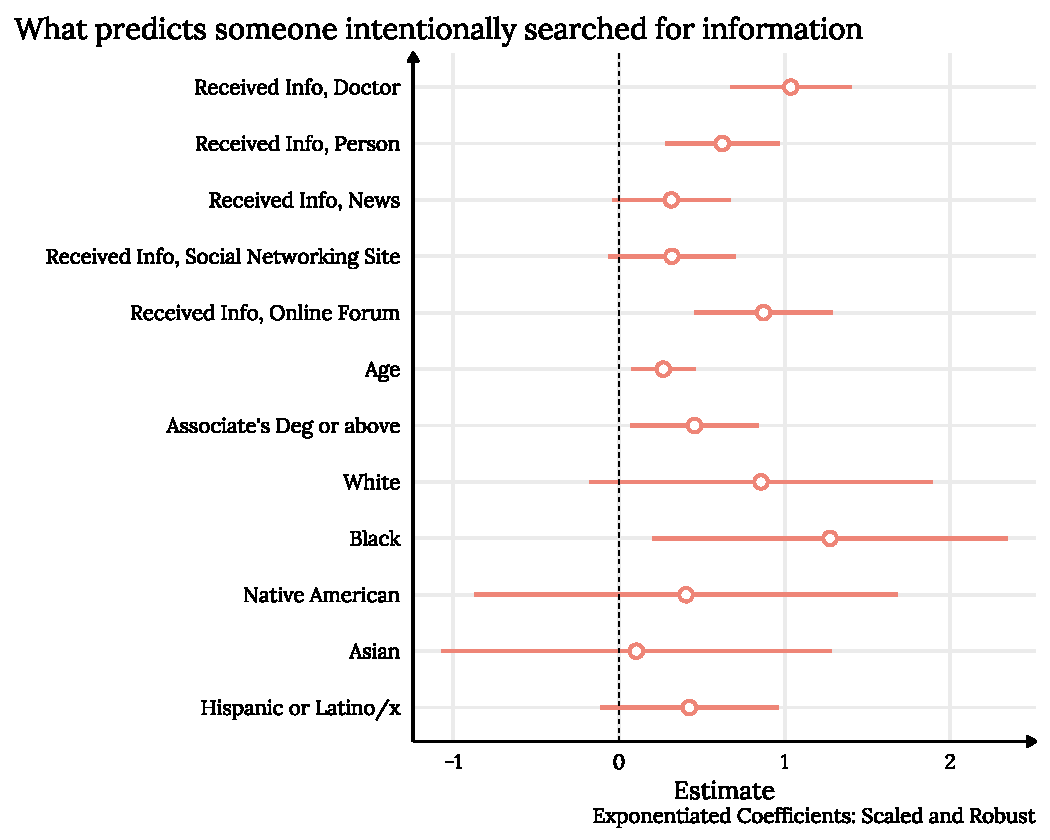
\includegraphics[width=0.8\linewidth]{figs/paper2/plot-model-1-1}}
\caption{What predicts someone intentionally searched for information? Plot of Coefficients}\label{fig:plot-model-1}
\end{figure}

Table \ref{tab:table-model-1} provides the results of my logistic regression
analysis predicting whether someone sought information about COVID-19. These
initial results suggest similar results for each modality of information
delivery: each mode of receiving information whether from a doctor, a person,
the news, a social networking site, or an online forum, all increase the odds of
seeking out information. For example, respondents who had received information
from a doctor or other medical professional were 2.82 (odds ratio = \(exp(\beta
k)\), \emph{p} \textless{} 0.001) times more likely to seek out information over
someone who had not. Similarly, respondents who had received information from `a
person like friend, neighbor, or family member that [they] know' were 1.87
(\emph{p} \textless{} 0.001) times more likely to seek out information over
someone who had not received information from a person like that. Interesting,
those who had received information from an online discussion group, listserv, or
other online forum including a Facebook group or subreddit were 2.39 (\emph{p}
\textless{} 0.001) times more likely to search out more information than someone
who had not. While most demographic variables do not seem to have a strong
effect on whether someone sought out information about the COVID-19 vaccine, a
few key variables had strong associations.  Respondents who are older are more
likely to seek information; The odds are about 3\% higher when age is equal to x
+ 1 relative to x, possibly indicating a generational effect of information
seeking patterns (\emph{p} \textless{} 0.01). Additionally, those who were more
educated, that is those with an Associate's degree or higher, were 1.58 more
likely to seek additional information than those without the degree (\emph{p}
\textless{} 0.05). And finally, there is evidence to suggest that the Black or
African American sample was more likely to seek out information, specifically:
Blacks were 3.58 times more likely to seek out information over non-Blacks
(\emph{p} \textless{} 0.05). Figure \ref{fig:plot-model-1} illustrates the
relationship between the coefficients and information seeking.

\hypertarget{information-search-modalities}{\subsection{Information Search Modalities}\label{information-search-modalities}}

\begin{table}[ht]

\caption{\label{tab:model-2-phi}Phi Coefficient ($\phi$) of binary association between each Information Search Vehicle}
\centering
\begin{tabular}{p{0.25\linewidth} p{0.10\linewidth} p{0.08\linewidth} p{0.12\linewidth} p{0.15\linewidth} p{0.12\linewidth}}\toprule
 & Person & Dr & Online Forum & SNS & Online Search \\\toprule
Person & \- &  0.28& 0.172& 0.275& 0.216 \\
Dr & \- &  \- &  0.192 & 0.152 & 0.098 \\
Online Forum& \- &  \- &  \- &  0.371& -0.073 \\
SNS & \- &  \- &  \- &  \- &  0.057 \\
Online Search& \- &  \- &  \- &  \- &  \\
\bottomrule
\multicolumn{6}{l}{\rule{0pt}{1em}Notes: SNS = Social Networking Site}\\

\end{tabular}
\end{table}

To further investigate how people search for information, I asked those who had
sought information out intentionally, ``How did you look for information about
the COVID-19 vaccine?'' Because respondents could select as many responses as
applicable, each response is recorded as a dichotomous variable. Table
\ref{tab:table-1-ind} reveals differences in the prevalence of usage of the
various information seeking modalities: Around 40\% of the sample has inquired
for information from a doctor, a person, or using online search tool (44\%,
42\%, 41\%), while my respondents used modalities like online forums (27\%) and
social networking sites (18\%) to seek out information at significantly lower
rates.

To investigate how each information search modality is related to each other
using the Phi Coefficient ($\phi$) of binary association between each
Information Search modality pair. The Phi coefficient can be interpreted like a
correlation coefficient, with numbers closer to -1 indicating a very strong
negative relationship and those closer to positive 1 indicating a very strong
positive relationship (Warrens 2008). Table \ref{tab:model-2-phi} shows the
results of these coefficients. Out of the five information search modalities
investigated, there is evidence that the modalities are distinctly different
concepts because most coefficients fall under 0.3, the general cutoff for
correlation coefficients to indicate a relationship. There does seem to be a
relationship between Online Forums and social networking sites, possibly due to
an individual's latent propensity to use online networks over in-person
networks. These coefficients indicate a weak relationship between any two
modalities of information search and that respondents in my sample utilize each
of these a little bit differently.

I find that indeed the most common modalities are asking a doctor, asking a
friend, and asking a search engine which provides evidence to reject the null
hypothesis for Hypothesis
\ref{hyp:drgooglefriend}. However, because the modalities 95\% confidence
intervals in Table \ref{tab:table-1-ind} are overlapping, I fail to reject 
the null Hypothesis \ref{hyp:online-vs-network}, that using an online search
engine was more commonplace than asking a friend.

\begin{table}[!h]

\caption{\label{tab:table-model-2}What predicts someone intentionally searched for information, by vehicle of information search}
\centering
\resizebox{\linewidth}{!}{
\begin{tabular}[t]{llllll}
\toprule
\multicolumn{1}{c}{ } & \multicolumn{5}{c}{Dependent Variable} \\
\cmidrule(l{3pt}r{3pt}){2-6}
  & Doctor & Person & Online Forum & Social Networking Site & Online Search\\
\midrule
\cellcolor{gray!6}{Received Info, Doctor} & \cellcolor{gray!6}{\num{1.942}***} & \cellcolor{gray!6}{\num{1.124}***} & \cellcolor{gray!6}{\num{0.181}} & \cellcolor{gray!6}{\num{0.540}**} & \cellcolor{gray!6}{\num{0.430}**}\\
Received Info, Person & \num{0.800}*** & \num{1.199}*** & \num{0.728}*** & \num{0.281} & \num{0.365}*\\
\cellcolor{gray!6}{Received Info, News} & \cellcolor{gray!6}{\num{0.437}**} & \cellcolor{gray!6}{\num{0.100}} & \cellcolor{gray!6}{\num{0.359}*} & \cellcolor{gray!6}{\num{0.514}*} & \cellcolor{gray!6}{\num{1.091}***}\\
Received Info, Social Networking Site & \num{-0.130} & \num{0.437}** & \num{-0.603}** & \num{0.731}*** & \num{1.272}***\\
\cellcolor{gray!6}{Received Info, Online Forum} & \cellcolor{gray!6}{\num{0.412}*} & \cellcolor{gray!6}{\num{0.263}+} & \cellcolor{gray!6}{\num{1.266}***} & \cellcolor{gray!6}{\num{0.974}***} & \cellcolor{gray!6}{\num{0.695}***}\\
Age & \num{0.002} & \num{0.001} & \num{-0.007} & \num{-0.003} & \num{0.029}***\\
\cellcolor{gray!6}{Associate's Deg or above} & \cellcolor{gray!6}{\num{0.542}**} & \cellcolor{gray!6}{\num{0.154}} & \cellcolor{gray!6}{\num{1.086}***} & \cellcolor{gray!6}{\num{1.344}***} & \cellcolor{gray!6}{\num{-0.952}***}\\
White & \num{0.631} & \num{0.245} & \num{0.009} & \num{0.559} & \num{0.012}\\
\cellcolor{gray!6}{Black} & \cellcolor{gray!6}{\num{0.366}} & \cellcolor{gray!6}{\num{0.208}} & \cellcolor{gray!6}{\num{0.608}} & \cellcolor{gray!6}{\num{0.646}} & \cellcolor{gray!6}{\num{0.357}}\\
Native American & \num{0.309} & \num{-0.696} & \num{0.209} & \num{0.762} & \num{-0.831}\\
\cellcolor{gray!6}{Asian} & \cellcolor{gray!6}{\num{-0.294}} & \cellcolor{gray!6}{\num{-0.566}} & \cellcolor{gray!6}{\num{-2.496}**} & \cellcolor{gray!6}{\num{-0.568}} & \cellcolor{gray!6}{\num{0.634}}\\
Hispanic or Latino/x & \num{0.324} & \num{0.116} & \num{0.529}* & \num{0.632}** & \num{-0.585}*\\
\cellcolor{gray!6}{Num.Obs.} & \cellcolor{gray!6}{\num{948}} & \cellcolor{gray!6}{\num{948}} & \cellcolor{gray!6}{\num{948}} & \cellcolor{gray!6}{\num{948}} & \cellcolor{gray!6}{\num{948}}\\
\midrule
$R_{McFadden}^2$ & \num{0.193} & \num{0.121} & \num{0.145} & \num{0.154} & \num{0.221}\\
\cellcolor{gray!6}{BIC} & \cellcolor{gray!6}{\num{1152.2}} & \cellcolor{gray!6}{\num{1237.6}} & \cellcolor{gray!6}{\num{1048.0}} & \cellcolor{gray!6}{\num{864.8}} & \cellcolor{gray!6}{\num{1104.6}}\\
Log.Lik. & \num{-524.709} & \num{-567.376} & \num{-472.576} & \num{-380.971} & \num{-500.907}\\
\bottomrule
\multicolumn{6}{l}{\rule{0pt}{1em}* p $<$ .05. ** p $<$ .01. *** p $<$ .001 (two-tailed test).}\\
\multicolumn{6}{l}{\rule{0pt}{1em}Raw, Unexponentiated Coefficients}\\
\end{tabular}}
\end{table}

I conduct a separate logistic regression for each search modality in Table
\ref{tab:table-model-2}. Modeling each response as a separate formula is useful
for interpretation, but there are important caveats: because each logistic
regression is on a different scale, one must not compare the magnitude of
coefficients between models. We can, however, use the direction and significance
of the coefficients to draw conclusions about these different forms of
information search modalities.

The first model in Table \ref{tab:table-model-2} predicts whether a respondent
sought information intentionally about COVID-19 vaccinations by asking their
doctor or another health professional. First and foremost, I find that those who
received information about COVID-19 vaccinations were 6.97 times more likely to
seek out more information from their doctor than those who had not (\emph{p}
\textless{} 0.001). However, receiving information from other modalities also
increased the odds of seeking out information from medical professions. Those
who received information from a person such as a friend or a relative were 2.23
times more likely to ask their doctor (\emph{p} \textless{} 0.001), while those
who received information from the news or television were 1.55 times more likely
(\emph{p} \textless{} 0.01). I also find that those who received information
from an online forum like a subreddit were 51\% more likely to ask their doctors
than those who had not (\emph{p} \textless{} 0.05). Finally, respondents with an
Associate's degree or higher were 72\% more likely to ask their doctor for
information on the COVID-19 vaccinations than those who held less education
(\emph{p} \textless{} 0.01).

The second model predicts whether a respondent sought information about COVID-19
vaccinations by asking a person like friend, neighbor, or family member that
they know. Only three coefficients in this model were significant and help us
draw any conclusions on who is most likely to activate their personal social
network for informational support. In this study, I find that receiving
information about the vaccine from a doctor, their personal network, or a social
networking site is associated with seeking out more information. Those who
received information from a doctor or other medical professional were 3.08 times
more likely to seek information from a person such as a friend (\emph{p}
\textless{} 0.001). Moreover, it seems that receiving information from your
personal social network, such as a friend or relative, is associated with
seeking information from those same people; in fact, I find that those who did
are 3.32 more likely to do so (\emph{p} \textless{} 0.001, see Table
\ref{tab:table-model-2}, ``Person'' model). Finally, the
respondents who received information about the vaccine on a social networking
site were 55\% more likely to seek information from their personal network than
those who had not (\emph{p} \textless{} 0.01). The unexpected result of this
model is that very few factors predict personal social network activation, and
this model has the lowest McFadden's R\^{2}, indicating possible omitted
variables. Possible omissions may include personality type, psychosocial
resources, and personal network composition. 

I also wanted to examine what factors were associated with posting in an online
discussion group, listserv, or other online forum like a Facebook Group or
Subreddit about COVID-19 vaccinations. This is conceptually different than
posting a query on a social networking site like Facebook or twitter where
identities are involved, but is theoretically more social friction than
searching on an internet search engine. I found that having received information
about the vaccine from your personal social network (such as a friend or
relative), the news, or an online forum was associated with higher odds of
querying an online forum. Specifically, receiving information from your personal
network is associated with 2.07 higher odds (\emph{p} \textless{} 0.001), from
news or television media with 1.43 higher odds (\emph{p} \textless{} 0.05), and
receiving information on an online forum associated with 3.55 higher odds
(\emph{p} \textless{} 0.001). Moreover, I found that those with an Associate's
degree or above were 2.96 times more likely to search for information on an
online forum (\emph{p} \textless{} 0.001). Finally, I found that
Hispanic-Latinos were about 70\% more likely to query an online forum than
non-Hispanics (\emph{p} \textless{} 0.05). However, there were also a few
variables that lowered the odds of posting in an online discussion group. First,
those who had received information from a social networking site were 45\% less
likely to query a forum than those who had not (odds ratio = \(1 - exp(\beta
k)\), \emph{p} \textless{} 0.01). Moreover, I found additional ethnoracial
effects: Respondents who claimed Asian ancestry were 92\% less likely to query
online forum (\emph{p} \textless{} 0.01).

The fourth model predicts whether an individual sought information about
COVID-19 vaccinations through posted queries on a social networking site such as
Facebook timeline, Twitter status update, or LinkedIn. Receiving information
about COVID-19 seems to be quite related to posting on social media. Those who
received information from their doctors had 1.72 higher odds of posting on a
social networking site (\emph{p} \textless{} 0.01), while those who received
their information from tv/news had 1.67 higher odds (\emph{p} \textless{} 0.05).
Furthermore, those who received information on social networking sites were more
likely to post queries on social networking sites (\(\beta\) = 2.08, \emph{p}
\textless{} 0.001). The respondents in our sample who received information from
online forums had 2.65 higher odds of posting queries on their social networking
platforms (\emph{p} \textless{} 0.001). I found a relationship between education
and posting on social networking sites as well; specifically, those with an
Associate's degree or above were 3.83 times more likely to post vaccination
queries on social networking sites than those with lower education (\emph{p}
\textless{} 0.001). Finally, I find that Hispanic-Latinos were 88\% more likely
to ask their connections on a social networking site about the COVID-19
vaccinations than non-Hispanics (\emph{p} \textless{} 0.01).

Searching for information using an online search engine such as Google or Bing
is theoretically the search modality with the least amount of social or
cognitive friction. Our descriptive statistics showed that not everyone used
this modality, with only 41\% of our sample (See Table \ref{tab:table-1-ind})
having sought information about the COVID-19 vaccines using online search
engines. My model reveals interesting patterns to help explain the variation. As
with previous models, receiving information of any kind increase the odds of
online search, though to varying magnitudes (Doctor: 1.54 odds; Person: 1.44
odds; News or Television: 2.98 odds; social networking site: 3.57 odds; Online
Forum: 2 odds). I also find that older respondents were more likely to search
online, with each addition year aged to yield 3\% higher odds of searching
online (\emph{p} \textless{} 0.001). The most interesting variations come from
what decreases the odds of online search. First, those with an Associate's
degree or higher were 61\% less likely to search online for questions about
COVID-19 than those with less educational attainment (\emph{p} \textless{}
0.001). In addition, I find that Hispanic-Latinos had 44\% lower odds of
searching online than non-Hispanics (\emph{p} \textless{} 0.05).

\hypertarget{vaccination-views}{\subsection{Choosing to be Vaccinated}\label{vaccination-views}}

\begin{table}[!h]

\caption{\label{tab:table-model-3}Does receiving or searching for information predict vaccination status?}
\centering
\begin{tabular}[t]{lc}
\toprule
  & Model 1\\
\midrule
\cellcolor{gray!6}{Received Info, Doctor} & \cellcolor{gray!6}{\num{1.049}*** (\num{0.301})}\\
Received Info, Person & \num{-0.206} (\num{0.242})\\
\cellcolor{gray!6}{Received Info, News} & \cellcolor{gray!6}{\num{0.108} (\num{0.247})}\\
Received Info, Social Networking Site & \num{-0.794}*** (\num{0.240})\\
\cellcolor{gray!6}{Received Info, Online Forum} & \cellcolor{gray!6}{\num{-0.321} (\num{0.248})}\\
Sought Info, Doctor & \num{1.386}*** (\num{0.341})\\
\cellcolor{gray!6}{Sought Info, Person} & \cellcolor{gray!6}{\num{0.570}* (\num{0.285})}\\
Sought Info, Social Networking Site & \num{0.710} (\num{0.466})\\
\cellcolor{gray!6}{Sought Info, Online Forum} & \cellcolor{gray!6}{\num{0.354} (\num{0.342})}\\
Sought Info, Online Search & \num{0.085} (\num{0.260})\\
\cellcolor{gray!6}{Age} & \cellcolor{gray!6}{\num{-0.018}+ (\num{0.011})}\\
Associate's Deg or above & \num{1.281}*** (\num{0.234})\\
\cellcolor{gray!6}{White} & \cellcolor{gray!6}{\num{1.122} (\num{0.767})}\\
Black & \num{0.808} (\num{0.799})\\
\cellcolor{gray!6}{Native American} & \cellcolor{gray!6}{\num{0.126} (\num{0.829})}\\
Asian & \num{1.555}+ (\num{0.918})\\
\cellcolor{gray!6}{Hispanic or Latino/x} & \cellcolor{gray!6}{\num{1.039}* (\num{0.505})}\\
Num.Obs. & \num{936}\\
\midrule
\cellcolor{gray!6}{$R_{McFadden}^2$} & \cellcolor{gray!6}{\num{0.261}}\\
BIC & \num{669.2}\\
\cellcolor{gray!6}{Log.Lik.} & \cellcolor{gray!6}{\num{-266.187}}\\
\bottomrule
\multicolumn{2}{l}{\rule{0pt}{1em}* p $<$ .05. ** p $<$ .01. *** p $<$ .001 (two-tailed test).}\\
\multicolumn{2}{l}{\rule{0pt}{1em}Raw, Unexponentiated Coefficients}\\
\end{tabular}
\end{table}

Finally, in Table \ref{tab:table-model-3}, I investigate whether there is a
relationship between information receiving and information seeking behaviors and
the choice to get vaccinated against COVID-19 through a logistic regression
model predicting Vaccination Outlook. I find that receiving information from a
doctor or other medical profession is associated with 2.85 odds of choosing to
receive a COVID-19 vaccination (\emph{p} \textless{} 0.001) and that seeking
information from a doctor also increases the odds of vaccination by 4 (\emph{p}
\textless{} 0.001). I find that my respondents who received information on a
social networking site like Facebook or Twitter about the vaccines were 55\%
\textbf{less likely} to choose to get vaccinated than those who received no
information through that modality (\emph{p} \textless{} 0.001). However, I did
find that those who reached out to family or friends with their concerns were
77\% more likely to become vaccinated (\emph{p} \textless{} 0.05). Furthermore,
my respondents who held an Associate's degree or above had 3.6 higher odds of
becoming immunized (\emph{p} \textless{} 0.001). And finally, I found further
ethnoracial differences in my sample. I found that Hispanic-Latinos had 2.83
higher odds of vaccination than non-Hispanics (\emph{p} \textless{} 0.05) and
that my Asian sample had 4.73 higher odds as well over non-Asians (\emph{p}  =
0.09). See Figure \ref{fig:plot-model-3} for a visual representation of how
these different coefficients are related to vaccination outlook. `Gender, Other'
is likely an outlier with an inflated effect here due to only 6 participants
being coded as `Other' for their gender. 

\begin{figure}[h]
{\centering 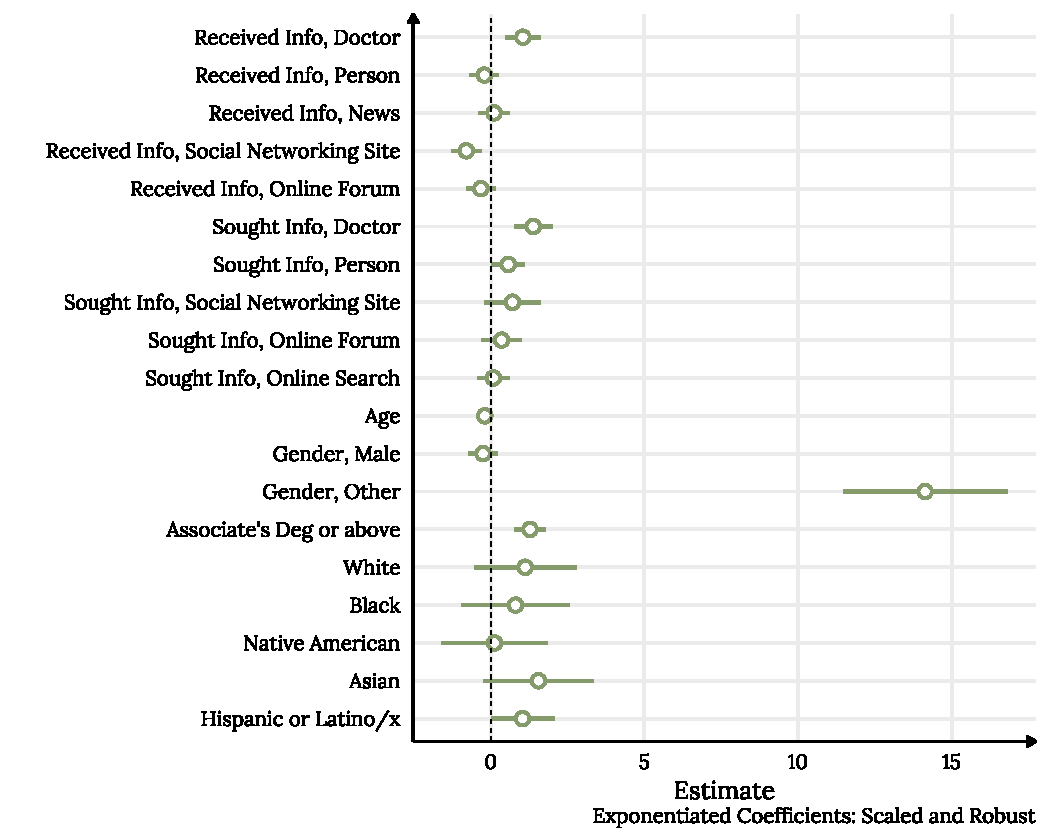
\includegraphics[width=0.8\linewidth]{figs/paper2/plot-model-3-1}}
\caption{Does receiving or searching for information predict vaccination outlook? Plot of Coefficients}\label{fig:plot-model-3}
\end{figure}

\hypertarget{discussion}{\section{Discussion and Conclusion}\label{discussion}}

Previous research in Sociology and Infodemiology has greatly failed to
distinguish between the activation of information seeking behaviors online and
offline. In this paper, I sought to uncover just how different various methods
of information search are and begin a line of research inquiry that investigates
the factors associated with each different modality. Finally, I also uncovered
how the different sources of information exposure and information search
modalities hold real world consequences through their associations with COVID-19
vaccination rates and intentions.

% TODO explain finding about online search being less prominent than social networks, though opposite to the theory. relate this to Rains work and how it may be the search for personalized or experiential information making the difference. 

I first find that being exposed to information about COVID-19 vaccinations from
any source increases the likelihood of searching out more information. I also
find important demographic differences in the overall propensity to seek out
information. First, I find that the older a respondent is, the more likely they
are to seek out information about COVID-19 vaccinations, possibly indicating a
larger information need by elderly populations overall, or a more pressing need
to search for information about the COVID-19 vaccinations because of the higher
risk of hospitalizations that older populations face \citep{turner_etal18}.
Furthermore, I find that those who are college educated were more likely to seek
out information; for the most part this trend can be observed in Table
\ref{tab:table-model-2} as well. Human Capital Theory \citep{mirowsky_ross98}
may help to explain this finding; this theory claims that higher education can
provides the skills to gain health-related knowledge and use this knowledge to
be proactive in their own lives. Finally, I find that my respondents who
identified as Black were more likely to seek out further information; this may
be explained by the maltreatment that African Americans have endured in the US
healthcare system \citep{baileyStructuralRacismHealth2017} which has led to
major distrust of the medical establishment among the population
\citep{center2019, murray15, bronson2014don}.
% TODO This is interesting speculation. Is there some way (in future studies) to further investigate this?

Table \ref{tab:table-model-2} further demonstrated important takeaways about how
individuals seek information. First, I find that the different information
seeking modalities queried in this survey are conceptually different and that
the utilization of different varies by demographic and information exposure
source. Overall, being exposed to information about COVID-19 vaccinations from
any source is associated with information seeking behaviors, though there are
key variations. First, if one received information from a doctor, they were
likely to search for information from a doctor; this may indicate an already
existing trusting relationship between patient and healthcare provider but it
may also indicate the healthcare provider taking initiative and emphasizing the
importance of the vaccine or the survey respondent seeking out information from
an expert. Another important finding is that if you received information from a
social networking site like Facebook or Twitter, you were less likely to query
Online Forums like Reddit or Facebook Groups; this may be an example of Uses and
Gratification Theory \citep{blumlerUsesMassCommunications1974}, where the two
online platforms may act as substitute sources of information and those who were
satisfied with the information they received on a social networking site didn't
have the need to seek out more information. Finally, the ethnoracial variations
exhibited in Table \ref{tab:table-model-2} likely demonstrate how cultural
attitudes around the trustworthiness of different sources of information affect
the utilization of different methods; for example, Asians seem to be less likely
to use online forums than non-Asians, while Hispanics are more likely to use
them than non-Hispanics. The internal variations between the different
information search modalities hint at different user profiles and may have major
repercussions on the quality of information they find and who is exposed to poor
quality information.

Given the rampant misinformation around COVID-19, its related vaccinations
\citep{pathakInfodemicsCOVID19Role2020, mottaHowRightLeaningMedia2020,
shahsavariConspiracyTimeCorona2020}, and the slowed rate of vaccinations in the
United States, it is important to uncover what relationship the different
sources of information exposure and information search modalities for COVID-19
vaccinations are associated with compliance with public health recommendations.
Table \ref{tab:table-model-3} demonstrated just how these different sources of
information exposure and information search modalities are associated with real
world consequences through COVID-19 vaccination rates and intentions. The first
takeaway is that receiving or seeking information from a doctor or other medical
profession was associated with higher likelihood of completed or planned
vaccinations. While blanket advice like ``Healthcare Providers should recommend
the vaccine to their patients'' would be less than totally effective because of the declining
number of Americans with a primary care doctor \citep{levine_etal20}, increasing
trust in the institution of medicine seems to remain a strong predictor of
vaccinations. A second major takeaway is that receiving information from a
Social Networking Site like Facebook timeline or Twitter status update was
significantly associated with lower vaccination rates. While we do not know what
exact information was absorbed on these platforms, the lower odds of vaccination
indicate that it was not positive. Much has been attempted between 2020 and 2022
to curb vaccine misinformation on these social networking platforms
\citep[see][for an early example]{bowman20}; however, I find evidence that these
social networking platforms nevertheless have a measurable negative impact.
Finally, this study also contributes to the conversation on ethnoracial and
educational differences in vaccine hesitancy. I find in my sample that
Hispanic-Latinos and Asians were more likely than non-Hispanics and non-Asians
to receive or plan to receive a vaccination against COVID-19 (Table
\ref{tab:table-model-3}). Research in this area has mixed results, with some
studies showcasing consistent findings to these
\citep{bagasra_etal21,king_etal21}, while others show that Whites have the
lowest levels of vaccine hesitancy and many minorities are much more hesitant
\citep{momplaisir_etal21, foxworth21}. My finding that college-educated
respondents were more likely seek vaccination is largely consistent with the
broader literature m\citep{khairat_etal22}, though again there are many
variations depending on the vaccine in question and study context
\citep{siddiqui_etal13}.

Previous research has greatly failed to distinguish between the activation of
information seeking behaviors online and offline and largely focuses on the
information that is sent to consumers [push], seeing people as passive receivers
of information. In this paper, I instead focus on individuals as active agents
in their search for information to begin a line of research inquiry that
investigates the factors associated with the various methods of information
search.

Given the large swaths of both misinformation and disinformation regarding
COVID-19 \citep{pathakInfodemicsCOVID19Role2020, mottaHowRightLeaningMedia2020,
shahsavariConspiracyTimeCorona2020} and the measurable impacts this
misinformation has had on pandemic-related health behaviors
\citep{loombaMeasuringImpactCOVID192021, greene_murphy21}, COVID-19 provides an
ideal study to investigate how we choose to search for information that affects
both our own lives and the lives of others.

This paper has provided several key findings that can be used to motivate policy
interventions for the COVID-19 vaccination campaigns and in the future for other
information campaigns. However, these findings are not to be taken out of the
context of their limitations. This paper is built off a small survey sample
(948) that was hosted online and anonymously through MTurk, a service that
provides people with micro-jobs. Because of the structure of the website,
respondents are incentivized to fill out surveys and other tasks as quick as
possible and there is no incentive for respondents to be honest in their
responses. For the same reason, there were many responses that were poor quality
and removed from the sample before analysis. However, each of these limitations
are common critiques of survey research as a whole. Even given these
limitations, the finding of this paper are interesting and timely contributions
to the literature.

Overall, this research project is important because the modalities used in
information search impacts the information and quality of information found. By
looking at how individuals search, I aimed to identified pain points and focus areas
for future interventions (receiving information online; ethnoracial variations) 
in the misinformation process.
\newpage
\section{References}
\begin{singlespace}
\printbibliography[heading=none] % print section bibliography
\end{singlespace}
\end{refsection}
\newpage
\begin{singlespace}
\hypertarget{appendix-1-survey-questions}{%
\section{Appendix 1: Survey Questions}\label{appendix-1-survey-questions}}

\begin{center}\rule{0.5\linewidth}{0.5pt}\end{center}

\emph{Q181}: Now, we're going to transition a bit to ask you about the information you received during the Covid-19 pandemic.

\begin{center}\rule{0.5\linewidth}{0.5pt}\end{center}

\emph{Q170}: In the past 12 months, without searching for it, did you receive information about the Covid-19 vaccine from \ldots{} (check all sources you received information from)

\begin{itemize}
\tightlist
\item
  your doctor or other health professional? (1)
\item
  a person like friend, neighbor, or family member that you know ? (9)
\item
  From television news channel or the newspaper? (10)
\item
  From an online discussion group, listserve, or other online forum including a Facebook group or subreddit? (11)
\item
  From a social networking site such as Facebook timeline, Twitter status update, or LinkedIn? (12)
\item
  Other (13) \_\_\_\_\_\_\_
\end{itemize}

\begin{center}\rule{0.5\linewidth}{0.5pt}\end{center}

\emph{Q171}: And how about you yourself intentionally looking for information about a Covid-19 vaccine? Such information can include things such as advice, clarification, facts, and experiences.

\begin{itemize}
\tightlist
\item
  Yes (4)
\item
  No (5)
\end{itemize}

\begin{center}\rule{0.5\linewidth}{0.5pt}\end{center}

\emph{Q172}: How did you look for information about the Covid-19 vaccine?

\begin{itemize}
\tightlist
\item
  Asking a person like friend, neighbor, or family member that I know (1)
\item
  Asking my doctor or another health professional (4)
\item
  Posted queries in an online discussion group, listserve, or other online forum like a Facebook Group or Subreddit (5)
\item
  Posted queries on a social networking site such as Facebook timeline, Twitter status update, or LinkedIn (6)
\item
  Searched for my question using an online search engine such as Google or Bing (7)
\item
  Other (8) \_\_\_\_\_\_\_\_\_\_\_
\end{itemize}

\begin{center}\rule{0.5\linewidth}{0.5pt}\end{center}

\emph{Q173}: What sort of information did you search for?
Separate different topics with a comma or semi-colon.

\begin{center}\rule{0.5\linewidth}{0.5pt}\end{center}

\emph{Q174}: How useful was the information you found?

\begin{itemize}
\tightlist
\item
  Extremely useful (22)
\item
  Very useful (23)
\item
  Moderately useful (24)
\item
  Slightly useful (25)
\item
  Not at all useful (26)
\end{itemize}

\begin{center}\rule{0.5\linewidth}{0.5pt}\end{center}

\emph{Q175}: Did the information you learned affect your decision to get vaccinated against Covid-19?

\begin{itemize}
\tightlist
\item
  Yes (39)
\item
  No (40)
\end{itemize}

\begin{center}\rule{0.5\linewidth}{0.5pt}\end{center}

\emph{Q179}: Did you receive a Covid-19 vaccine?

\begin{itemize}
\tightlist
\item
  Yes (9)
\item
  No (10)
\item
  I'm unsure or would not like to respond (11)
\end{itemize}

\begin{center}\rule{0.5\linewidth}{0.5pt}\end{center}

\emph{Q180}: Do you plan to receive a vaccine for the prevention of the Covid-19 virus?

\begin{itemize}
\tightlist
\item
  Definitely not (9)
\item
  Probably not (10)
\item
  Might or might not (11)
\item
  Probably yes (12)
\item
  Definitely yes (13)
\item
  I would not like to respond (14)
\end{itemize}

\begin{center}\rule{0.5\linewidth}{0.5pt}\end{center}

\emph{gender}: What is your gender?

\begin{itemize}
\tightlist
\item
  Male (1)
\item
  Female (2)
\item
  Other (3) \_\_\_\_\_\_\_\_\_\_\_\_\_\_\_\_
\item
  Prefer not to say (4)
\end{itemize}

\begin{center}\rule{0.5\linewidth}{0.5pt}\end{center}

\emph{hispanic}: Are you Hispanic, Latino/a/x, or Latin American Origin?

\begin{itemize}
\tightlist
\item
  Yes (1)
\item
  No (2)
\end{itemize}

\begin{center}\rule{0.5\linewidth}{0.5pt}\end{center}

\emph{race}: What is your race? If you are ``mixed race,'' select all that apply.

\begin{itemize}
\tightlist
\item
  White (1)
\item
  Black or African American (2)
\item
  American Indian or Alaskan Native (3)
\item
  Asian (please specify): (4) \_\_\_\_\_\_\_
\item
  Other (please specify): (5) \_\_\_\_\_\_\_
\item
  Prefer not to say (6)
\end{itemize}

\begin{center}\rule{0.5\linewidth}{0.5pt}\end{center}

\emph{educ}: What is the highest level of education that you have completed?

\begin{itemize}
\tightlist
\item
  Less than high school (1)
\item
  High school graduate (2)
\item
  Some college (3)
\item
  Associate's or Technical degree (4)
\item
  Bachelor's degree (5)
\item
  Graduate or professional degree (6)
\end{itemize}

\begin{center}\rule{0.5\linewidth}{0.5pt}\end{center}

\emph{income}: We would be interested to know roughly what your total household income
before taxes is. We mean income from all sources, including welfare, stock
dividends, other household members' income, etc. In 2020, in which bracket did your total family income fall?

\begin{itemize}
\tightlist
\item
  Under \$1,000 (1)
\item
  \$1,000 to \$9,999 (2)
\item
  \$10,000 to \$19,999 (3)
\item
  \$20,000 to \$29,999 (4)
\item
  \$30,000 to \$39,999 (5)
\item
  \$40,000 to \$49,999 (6)
\item
  \$50,000 to \$59,999 (7)
\item
  \$60,000 to \$74,999 (8)
\item
  \$75,000 to \$89,999 (9)
\item
  \$90,000 to \$109,999 (10)
\item
  \$110,000 to \$129,999 (11)
\item
  \$130,000 to \$149,999 (12)
\item
  \$150,000 or over (13)
\item
  Don't know (14)
\end{itemize}

\begin{center}\rule{0.5\linewidth}{0.5pt}\end{center}

\emph{age}: What is your age? (in years)

\end{singlespace}


\begin{refsection} % refsection environment
\hypertarget{paper-3}{\chapter{Social Norms under Uncertain Times: A dynamic study of Stay-At-Home and Vaccination Rates During the COVID-19 Pandemic}\label{paper-3}}

\hypertarget{abstract-1}{\section{Abstract}\label{abstract-1}}

My final article takes a deeper dive into the formation of social norms
governing health behaviors in cases of extreme uncertainty using the cases of
both stay-at-home rates and vaccination rates as responses to public health
recommendations to mitigate the COVID-19 pandemic. Using theories like
associative diffusion and the integrated theoretical framework of norms, I test
models of behavioral adaption to public health recommendations and patterns of
complex contagion (the need for repeated exposures to something novel for it
to diffuse) using linear mixed effects models. These models show that complex
contagion is a valid framework for the social contagion of new norms during
COVID-19. Importantly, I find a novel moderating effect of signal discordance,
the contextual diversity of signals received by an ego. If there is diversity in
the information received by an ego, contagion is less likely to occur. This
paper shows that the contagion process cannot be fully understood without
looking at the context of each exposure to a contagion within the range of
contagions one experiences.

Keywords: Social Networks, Complex Contagion, Social Norms, Health Behavior, Diffusion

\hypertarget{background}{\section{Background}\label{background}}

After spreading around the world in a matter of months, the coronavirus
(COVID-19) became a leading cause of death in the United States. Although the
Centers for Disease Control and Prevention (CDC)
\citeyearpar{centersfordiseasecontrolandpreventionHowProtectYourself2020}
proposed several potential mitigation strategies, the method of mitigation that
received the most national attention is the call to stay-at-home and social
distance for non-essential workers. CDC officials and front line health care
professionals advise that the best way to prevent exposure to the virus is to
stay-at-home and avoid close contact with people.

A second strategy pushed by the CDC, once available, was to receive vaccination
to prevent the effects of the COVID-19 virus if infected. Vaccinations like
Pfizer-BioNTech (Comirnaty, tozinameran, BNT162b2), and Janssen/Johnson \&
Johnson, Moderna (mRNA-1273) started receiving approval for emergency use
authorization by the United States Food and Drug Administration (FDA) in
December 2020.

Although these public health interventions were pushed by policy makers
throughout 2020 and 2021, policy makers often struggle to promote public
adoption of policies that rely on the publics' willingness to adjust their
current `risky' behaviors to less-risk behaviors based on scientific facts. The
lack of adaption to newly recommended behaviors is partially due to the
variation in how individuals came to understand the threats of the disease
\citep{akpanAssociationWhatPeople2021, bailey_etal20}, but also due to habitus:
the ingrained habits, skills and dispositions of individuals and groups
\citep{bourdieu77}. Habitus shapes how individuals perceive different social
interactions and norms and shape how they adopt different policies, leading to
different social outcomes and a divergence of attitudes
\citep{scottarthur_etal21, williams95, madeira_etal18}.

There is little research on stay-at-home rates, especially in cases of pandemics
or disasters. Though research on the causes of population mobility did expand
after the onset of the COVID-19 pandemic
\citep{bargainTrustCompliancePublic2020, bourassaStatelevelStayathomeOrders2020,
bourassaSocialDistancingHealth2020, grossmanPoliticalPartisanshipInfluences2020,
haggerPredictingSocialDistancing2020, hillBloodChristCompels2020,
hillNastiestQuestion, hillLoveThyAged2021,huynhDoesCultureMatter2020}, most
research focused on unchanging cultural determinants of the reduction in
stay-at-home rates. For instance, \citet{gibbons_etal21} finds that social
capital had spatially inconsistent effects on stay-at-home rates. Instead of
focusing on cultural relationships with stay-at-home rates, this paper will
instead focus on the dynamic nature of population mobility across population
networks.

There is more research on vaccine uptake
\citep{schmidBarriersInfluenzaVaccination2017} because of increased hesitancy
and anti-vaccination movements over previous decades
\citep{baumgaertnerInfluencePoliticalIdeology2018,
hornseyDonaldTrumpVaccination2020, johnsonOnlineCompetitionPro2020,
whiteheadHowCultureWars2020}. While some studies use social network analysis to
study the discussions for an against vaccinations online
\citep{milaniVisualVaccineDebate2020}, vaccination rates are a great way to
investigate the establishment of new social norms. First, vaccination uptake is
measurable with stable information tracking infrastructure and vaccination rates
are varied across locations and time. Secondly, because vaccines have become
politicized \citep{mottaRepublicansNotDemocrats2021,
mottaIdentifyingPrevalenceCorrelates2021}, the social contagion effects can be
studied.

This article researches the formation of social norms governing health behaviors
in cases of extreme uncertainty during the COVID-19 pandemic. Using theories of
complex contagion, associative diffusion and the integrated theoretical
framework of norms, I test how these health behaviors are outcomes of contagion
and discordance of signals, as well as other factors affecting associations like
religious and political conservatism, attention to television media sources, and
online norms as measured by information-search behaviors.

Before outlining my
central hypotheses, I offer an overview of the current state of the social
contagion literature. After that, I will outline how I compiled this unique
longitudinal data set from Google, the CDC, Facebook and other sources and how I
define and calculate signal and discordance, two key independent variables for
this paper. To model stay-at-home and vaccination rates, I use linear mixed
effects models with random effects as a longitudinal model of contagion. After
interpreting the results of the models, I discuss the implications of these
findings for the sociological understanding of social contagion and the
formation of social norms.

\hypertarget{the-social-contagion-model}{\subsection{The Social Contagion Model}\label{the-social-contagion-model}}

Individuals engage with each other and their distributed ties to create
community contexts where norms, beliefs, and values circulate. These clusters of
interaction are called social networks, and if ``each person continues to
interact primarily with others nearby in space, the forces of conformity will be
strongest locally, leading to the emergence of clusters of people sharing
similar behavior'' \citep{kitts_shi18}. This community interaction ultimately
leads to converged communities of belief structures with variations in how much
they diverge from the norm \citep{cullumCulturalEvolutionInterpersonal2007,
lataneExperimentalEvidenceDynamic1996, okadaStructureCulturalRejection2017}.

``Culture'' diffuses through communities and social networks. Information and
opinions spread \citep{bond_etal12,
fowler2010cooperative,klarEffectNetworkStructure2017}, behaviors are adopted
\citep{aralExerciseContagionGlobal2017, centolaSpreadBehaviorOnline2010,
centolaExperimentalStudyHomophily2011,christakis2008collective,rosenquist2010spread},
and there are patterns of health contagion 
\citep{cacioppo2009alone,christakisSpreadObesityLarge2007}. However, ``different
things spread in different ways and to different extents'' \citep[p.
563]{christakisSocialContagionTheory2013} and when modeling diffusion and
contagion, we must be very specific about our scope conditions as they are
relevant to our theory and not to cross theories to infer connections where they
may not exist \citep{kitts_quintane20}.

Most of the diffusion literature does not focus on establishment of new norms
but the adoption of culture and specific deviant behaviors \citep[see][for an
exception]{centolaSpontaneousEmergenceConventions2015}.
\citet{dellapostaWhyLiberalsDrink2015} outline how the spread of culture and
behavior is tied to network autocorrelation, or ``the tendency for people to
resemble their network neighbors.'' They show that the distance between two
agents in sociocultural space can determine the likelihood of the adoption of a
new behavior. Like \citet{axelrodDisseminationCultureModel1997}, this outlines
how the local convergence of close network actors becomes amplified and can lead
to global polarization between groups.

Outdated models found in early public health research claim that information
about the risks of behaviors will lead to changes in behaviors to mitigate those
said risks \citep[e.g.][]{flay_etal80}. However, while this model can be valid
in specific cases, more research has shown how the risks themselves do little to
motivate behavioral change \citep{witte_allen00,wolburg06}. Often, an appeal to
fear is found to be a major driver of the adoption of information campaigns and
some research has shown that ``social network exposure to COVID-19 cases shapes
individuals'' beliefs and behaviors concerning the coronavirus''
\citep{bailey_etal20}. Because of this, it is logical that higher local
incidences of infection would inspire fear and increase adherence to public
health measures according to this older model.

\begin{hyp2}[H\ref{hyp:infection}] \label{hyp:infection}
 Relatively higher local rates of infection will lead to increased time spent in residence and increase vaccination uptake
\end{hyp2}


\hypertarget{complex-contagion-and-discordance}{\subsection{Complex Contagion and Discordance}\label{complex-contagion-and-discordance}}

\citet{centolaComplexContagionsWeakness2007} theorize that simple contagions are
not enough to spread behavioral change. Simple contagions are those in which
only one point of contact is needed to receive contagion, like with infectious
disease or to learn simple bits of information. Centola and Macy
\citeyearpar{centolaComplexContagionsWeakness2007}'s large contribution was the
theorizing of complex contagions, those that require ``independent affirmation
or reinforcement from multiple sources'' (p. 703) and is not based on the number
of exposures but the number of sources of exposure. In the case of behavioral
contagion, this means that the behavior must be reinforced through witnessing
multiple alters perform this behavior before contagion can take effect.

In the case of stay-at-home rates or vaccination rates, this theoretically means
that a person exposed to many sources of the same signal (high, medium, low
rates) will be more likely to adopt the behavior based on the reinforcement from
the multiple sources of exposure. As norms are inherently social, I theorize
that we can see complex contagion happening in real time with the following
hypothesis:

\begin{hyp2}[H\ref{hyp:direction}] \label{hyp:direction}
Increased average time spent in residence (signal direction) from alters will have a positive effect on stay-at-home rates the ego-county; increased vaccine uptake by alters will have a positive effect on vaccine uptake for the ego-county
\end{hyp2}
% TODO I think I ``get'' this, but could you define ``ego county''? Also, why not just look at the effect of alter's behavior on ego's behavior (why does the county come into the framework)? Do you mean {the subset of ego's alters who live in the same county as ego}?

To make the contagion more complex, different sources of exposure
(county-alters) adhere to CDC recommendations to stay-at-home at differing
rates. Whereas one county-alter may be greatly increasing its time in residence,
another may have made little change. When the majority of alters is in
concordance with each other, the signal to the ego is reinforced and more
impactful on the ego. When these signals are mixed with high variance from
different sources, agreement is low and makes the behavioral change less likely.
For this paper, I theorize that a new concept of `discordance' must be
considered as impacting complex contagion. Discordance is the variance of
signals received by an alter; high discordance prevents reinforcement while low
discordance (concordance) enables complex contagion. Instead of adopting a
`majority' rules attitude, this means that the more discordance perceived by an
ego, the less likely the alters will have any effect on the ego. I theorize that
the behavior of a county-alter will be correlated with the behavior
of another county-ego if the county-ego receives highly discordant signals, as
seen in Figure \ref{fig:dag}.

\begin{hyp2}[H\ref{hyp:discordance}] \label{hyp:discordance}
The effect of signal direction on time spent in residence and vaccine uptake will be moderated by diversity in signals (discordance)
\end{hyp2}

\begin{figure}
{\centering 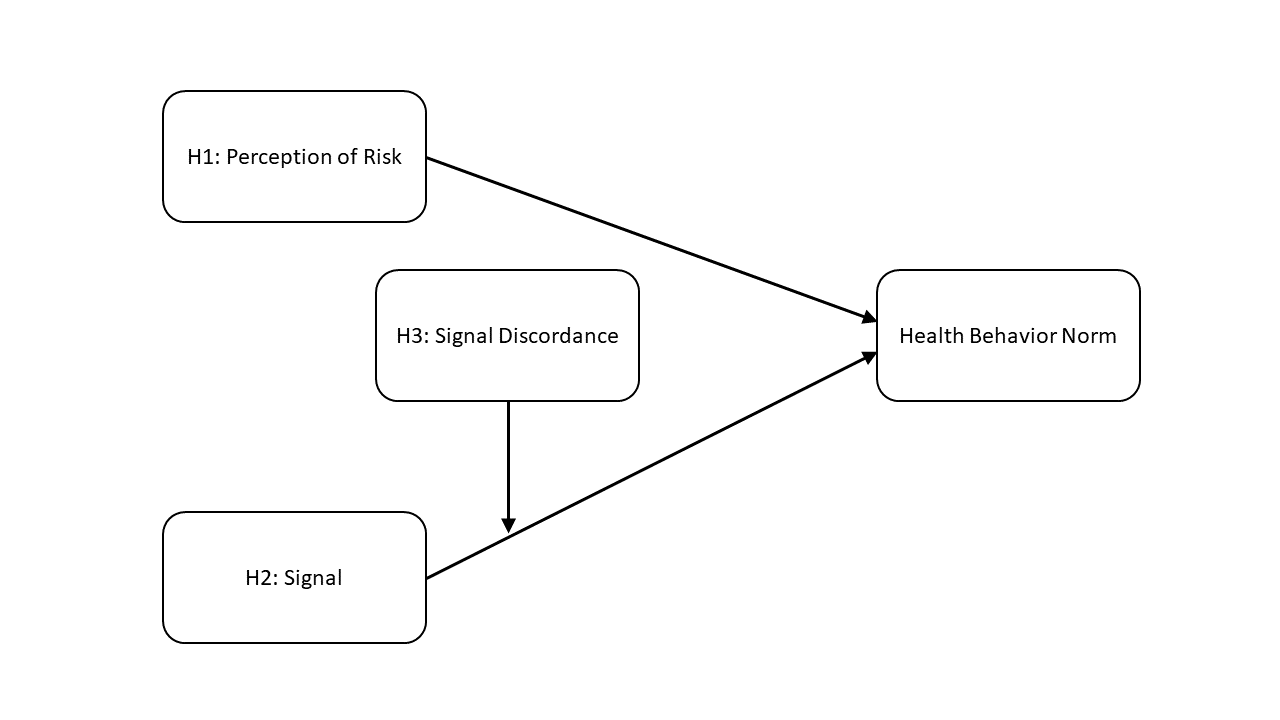
\includegraphics[width=0.8\linewidth]{figs/paper3/dag}}
\caption{Elaboratory Theoretical Model of Health Behavior Norms}\label{fig:dag}
\end{figure}

\hypertarget{associative-diffusion}{\subsection{Associative Diffusion}\label{associative-diffusion}}

While much of the social contagion literature, like the theories above, focuses
on structural boundaries and homophily as causes of how diffusion occurs,
\citet{goldbergSocialContagionAssociative2018} propose a disrupting alternative
mechanism. They argue that what actually diffuses during social contagion are
the perceptions about which beliefs or behaviors are compatible with one
another, what they call ``associative diffusion.'' This argument that culture
does not spread like a virus but instead is dependent on how belief structures
are connected to each other is important to test because norms around health
behaviors became politicized issues during the COVID-19 pandemic. This means
that the stay-at-home or vaccination behavior themselves were not contagious,
but the cognitive association of precisely what social distancing or vaccination
uptake \emph{meant} were spreading between populations of individuals. Moreover,
as \citet{houghton20} outlines, diffusants, the things that are diffusing
through a population, are not independent of each other \citep{mason_etal07}.
When we take into account the interdependence between different beliefs that are
diffusing, such as COVID-19 is a hoax, social distancing saves lives, the
COVID-19 vaccine includes a microchip to control your thoughts, and lockdown is
against the rights guaranteed in the US constitution, we can imagine how these
various diffusants become associated together into structures of belief through
schemas of perception \citep{houghton20}. While this cognitive theory of
cultural variation is difficult to test, the theory it supplies provides a solid
framework for how behavioral norms formed during the pandemic.

Individuals look to norms to regulate behavior, avoid deviance, and to maintain
order \citep{horneNormsIntegratedFramework2020,
shepherdStructurePerceptionHow2017}. When they realize they don't have a
normative set of responses in their cultural toolkit to respond to an unfamiliar
situation they are presented with, individuals look to the other sources in
their ``community'' to mimic behavior, such as high-status individuals,
institutions, and members of their social network. I theorize that individuals
look towards their physical community, to their social network, popular media,
established norms that they may find online through search, and to the real
threat of infection (what would happen if I do nothing about this norm).
Following both the Integrated Theoretical Framework of Norms
\citep{horneNormsIntegratedFramework2020} and associative diffusion
\citep{dellapostaWhyLiberalsDrink2015, goldbergSocialContagionAssociative2018},
I theorize that individuals interpret signals from their ``community'' through
their cognitive biases and behavioral predispositions to determine their
formation of new behavioral norms.

There is some evidence I can draw upon to support the associative diffusion
framework. For instance, there is a central conflict between religious and
scientific ideologies which I theorize leads more religious counties to reject
the stay-at-home order and vaccines
\citep{evansReligionScienceEpistemological2008} because the associative
diffusion of these behaviors pits public health recommendations against
religious ideologies. Furthermore, as COVID-19 has become a politically
polarizing issue \citep{ternullo22}, conservative ideology and a general
mistrust of ``big government'' \citep{frank2007, gauchat2008} are likely to lead
to resistance to the government and scientific guidance.

\hypertarget{data-and-methods}{\section{Data and Methods}\label{data-and-methods}}

This article draws on two unique longitudinal datasets that I compiled for this
analysis from sources like Facebook, Google, CDC, and more. Because the
different datasets were on different scales (individual, zip-code, county,
state, designated market area) and time points (cross-sectional, longitudinal),
there was extensive data wrangling that had to be done to prepare these data for
statistical analysis. The steps taken to prepare each of the different model
features and where the data was sourced from is therefore covered in the
following sections before diving into modeling specifications.

\hypertarget{stay-at-home-rates}{\subsection{Stay-at-Home Rates}\label{stay-at-home-rates}}

\begin{table}[!ht]

\caption{\label{tab:google-desc-table}Descriptive Statistics for Stay-at-Home Models (county-level)}
\centering
\begin{tabular}{lrrrr}
\toprule
  & min & max & mean & sd\\
\midrule
Percent White & \num{0.14} & \num{0.98} & \num{0.81} & \num{0.15}\\
Percent College Graduates & \num{0.08} & \num{0.75} & \num{0.26} & \num{0.10}\\
Percent over 65 & \num{6.60} & \num{56.70} & \num{16.90} & \num{4.05}\\
Median Income & \num{28951.00} & \num{142299.00} & \num{59773.61} & \num{15264.50}\\
Monthly Unemployment Rate & \num{1.40} & \num{34.60} & \num{8.12} & \num{4.00}\\
Percent of GOP votes, 2016 & \num{0.08} & \num{0.90} & \num{0.57} & \num{0.15}\\
Percent Evangelical Christian & \num{0.00} & \num{0.67} & \num{0.20} & \num{0.14}\\
'Fox News' Trend & \num{0.00} & \num{204.08} & \num{29.59} & \num{16.94}\\
'Social Distancing' Trend & \num{0.00} & \num{500.00} & \num{20.64} & \num{25.36}\\
'Covid Conspiracy' Trend & \num{0.00} & \num{825.00} & \num{42.51} & \num{80.44}\\
Covid Case Rate & \num{0.00} & \num{343.71} & \num{21.17} & \num{27.44}\\
Week Number & \num{0.00} & \num{43.00} & \num{23.14} & \num{11.77}\\
Movement Signal & \num{-2.06} & \num{26.44} & \num{8.31} & \num{4.22}\\
Movement Discordance & \num{0.15} & \num{11.05} & \num{2.22} & \num{0.80}\\
\bottomrule
\multicolumn{5}{l}{\rule{0pt}{1em}Raw values presented in table. Values in models are normalized.}\\
\multicolumn{5}{l}{\rule{0pt}{1em}Notes: 1,375 counties, March 02 through December 28, 2020.}\\
\end{tabular}
\end{table}
%TODO define normalization, make sure its mentioned in the methods section

\begin{figure}
{\centering 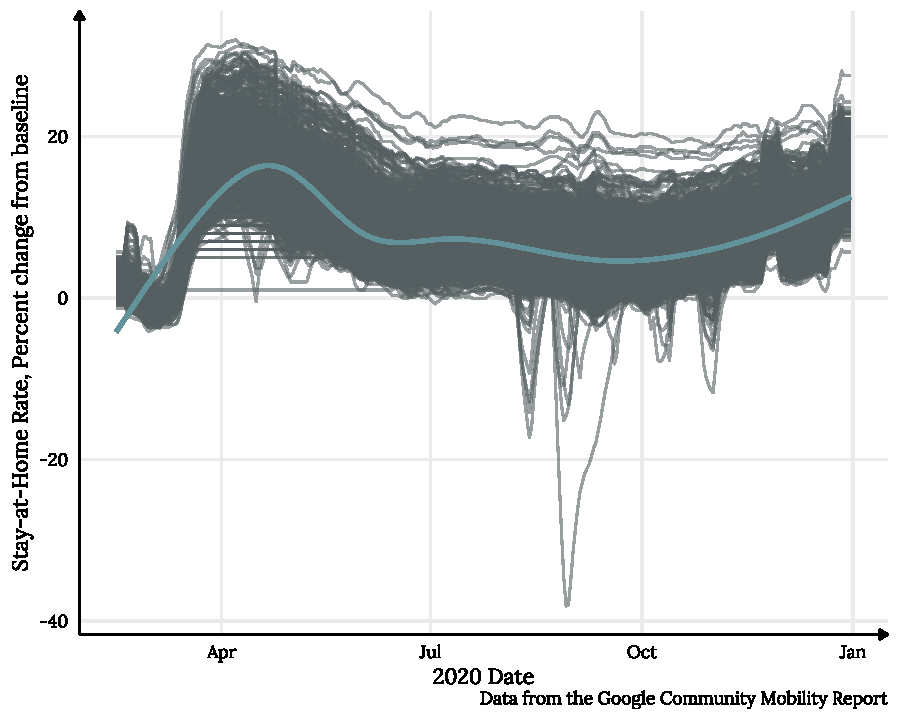
\includegraphics[width=0.8\linewidth]{figs/paper3/plot-google-1}}
\caption{Stay-at-Home Rates over Time}\label{fig:plot-google}
\end{figure}

My first dependent variable aims to operationalize behavioral norms as
stay-at-home rates with data from Google \citep{google2020}. While the Google
COVID-19 Community Mobility Reports include multiple measures of mobility based
on location and activity information, the change in time spent in residence most
closely aligns to an operationalization of an obedience to CDC and governor
orders, a new and emerging norm in 2020. The change in time spent in residence
variable represents percent change of time spent from Google Location History
within geographic areas that Google has designated as a residential area. These
data are aggregated to the county-level based on anonymized sets of data from
users who have turned on the Location History setting, which is off by default.
This means our sample is possibly skewed to people in the United States a) with
a mobile phone, b) with a Google account, and c) with knowledge of how to
synchronize their location history. Google has not made it clear whether there
are any weights in place to correct for these potential biases. Google
calculates the relative change in mobility in comparison to the median value of
movement in the area for the same corresponding day of the week, during the
5-week period Jan 3--Feb 6, 2020. As Google did not provide data on certain US
counties if they did not have sufficient statistically significant levels of
data, my final county sample is \emph{n} = 1375 (compared to the total
population of 3,107 US counties). Particular areas that are excluded in this
analysis include all counties in Alaska and DC, and over half of the counties in
North Dakota, South Dakota. A full list of excluded counties available upon
request. These data are longitudinal measures calculated by creating a moving
average of stay-at-home rates for each county (rolling window width = 7 days)
and then sampling every Monday in the sample for 44 measures from March 02, 2020
through December 28, 2020.

\hypertarget{covid-vaccination-uptake}{\subsection{COVID vaccination uptake}\label{covid-vaccination-uptake}}

\begin{table}[!h]

\caption{\label{tab:vacc-desc-table}Descriptive Statistics for Vaccination Models (county-level)}
\centering
\begin{tabular}[t]{lrrrr}
\toprule
  & min & max & mean & sd\\
\midrule
Percent White & \num{0.08} & \num{1.00} & \num{0.83} & \num{0.17}\\
Percent College Graduates & \num{0.03} & \num{0.78} & \num{0.22} & \num{0.10}\\
Percent over 65 & \num{3.20} & \num{56.70} & \num{18.86} & \num{4.50}\\
Median Income & \num{21504.00} & \num{142299.00} & \num{53522.45} & \num{14312.25}\\
Monthly Unemployment Rate & \num{0.90} & \num{22.00} & \num{4.96} & \num{1.95}\\
Percent of GOP votes, 2020 & \num{0.09} & \num{0.94} & \num{0.64} & \num{0.16}\\
Percent Evangelical Christian & \num{0.00} & \num{1.31} & \num{0.22} & \num{0.16}\\
'Fox News' Trend & \num{5.00} & \num{405.88} & \num{72.12} & \num{27.38}\\
'Covid-19 vaccine' Trend & \num{0.00} & \num{755.56} & \num{74.67} & \num{70.33}\\
'Covid Conspiracy' Trend & \num{0.00} & \num{2000.00} & \num{56.05} & \num{189.61}\\
Covid Case Rate & \num{0.00} & \num{998.58} & \num{22.79} & \num{27.23}\\
Week Number & \num{1.00} & \num{35.00} & \num{18.00} & \num{10.10}\\
Vaccination Signal & \num{0.00} & \num{62.84} & \num{19.62} & \num{14.84}\\
Vaccination Discordance & \num{0.00} & \num{22.40} & \num{5.26} & \num{3.62}\\
\bottomrule
\multicolumn{5}{l}{\rule{0pt}{1em}Raw values presented in table. Values in Models are normalized.}\\
\multicolumn{5}{l}{\rule{0pt}{1em}Notes: 2,819 counties, January 04 through August 30, 2021.}\\
\end{tabular}
\end{table}

\begin{figure}
{\centering 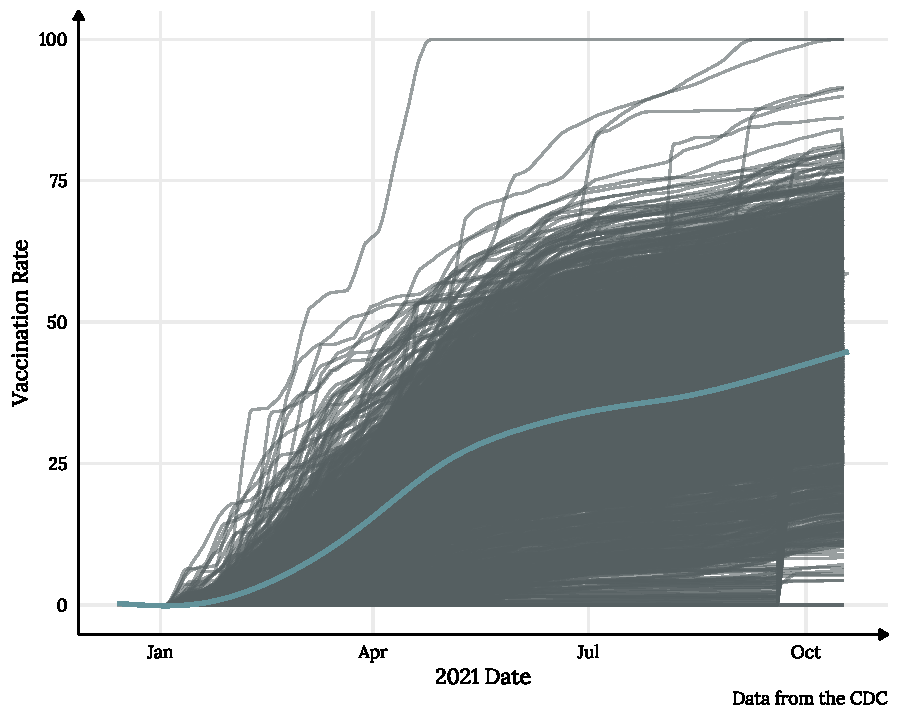
\includegraphics[width=0.8\linewidth]{figs/paper3/plot-vacc-1}}
\caption{Vaccination Rates over Time}\label{fig:plot-vacc}
\end{figure}
% TODO add which counties rose to 100% vaccination 

The second dependent variable aims to operationalize vaccination uptake through
vaccination rate information in the United States from January 2021 through
August 30 2021 \citep{cdcCOVID19Vaccination2021}. Data represents all vaccine
partners including jurisdictional partner clinics, retail pharmacies, long-term
care facilities, dialysis centers, Federal Emergency Management Agency and
Health Resources and Services Administration partner sites, and federal entity
facilities. Vaccination data is available for all US counties with the exception
of parts of California and Massachusetts, Hawaii, and Texas. In Texas and
Hawaii, no county level information is available, and California does not report
the county of residence for vaccinations when the county of residence has a
population less than 20,000 people. Finally, Massachusetts does not provide
vaccination data for Barnstable, Dukes, and Nantucket counties because of their
small populations. Therefore, my final county sample for vaccination rates is
\emph{n} = 2819 (compared to the total population of 3,107 US counties). A list
of included FIPS are available upon request. Vaccination rates are scaled with a
rolling mean with a rolling window width of seven days to smooth out intra-week
noise. I sample every Monday between January 2021 through August 30, 2021 for 35
total observations for each county.

\hypertarget{independent-variables-1}{\subsection{Independent Variables}\label{independent-variables-1}}

\hypertarget{network-signal}{\subsubsection{Network Signal}\label{network-signal}}

I utilize the likelihood of a friendship connection between counties to create a
county-level social network weighted by the probability of a tie. Using this
network and the two independent variables above, I examine how the vaccination
and stay-at-home rates of peer counties is contagious to the ego-county. To do
this, I first take the weighted average of each ego's network signals using
equation \eqref{eq:networksignal} where \texttt{x} denotes the vaccination and
stay-at-home rates of each alter county and \texttt{w} represents the likelihood
of a friendship connection between the ego county and each of their alters,
lagged by one week. This `signal' of norms gives us insight into the co-evolving
contagion patterns of the new social norm being established. The likelihood of
friendship connection comes from the ``Social Connectedness Index''
\citep{Bailey2018, facebook20} which indexes the social links between
geographies by the likelihood of Facebook friends. It is an aggregated measure
of Facebook friendship connections between counties. It corresponds to ``the
(relative) probability that two arbitrary Facebook users across two geographies
are friends with each other.'' The data is available at various geographic
aggregation levels, such as U.S. zip codes or entire countries. However, data is
only available at one time point because Facebook has found that although there
are individual changes in friendship connections over time, the aggregate
statistical probabilities of friendship remain stable. This measure is based on
user-provided information and real-time location-service data gathered by
Facebook. Facebook data has been shown to be highly representative of the U.S.
population and Facebook friendship links largely represent real-world
friendships \citep{bailey_etal18, jones_etal13}. The data has been tested to
show how initial COVID-19 hot spots are related to subsequent virus spread to
non-hot-spots, even after controlling for population density and geographic
distance \citep{Kuchler2020}.

\begin{equation}
signal = \frac{\sum_{i=1}^nw_ix_i}{\sum^n_{i=1}w_i} \label{eq:networksignal}
\end{equation}

\hypertarget{signal-discordance}{\subsubsection{Signal Discordance}\label{signal-discordance}}

The second independent variable, \emph{Signal Discordance}, builds on the
network signal but looks specifically at the extent to which a given ego-network
receives diverse contagion signals. Based on Hypothesis \ref{hyp:discordance},
that when the majority of alters is in concordance with each other, the signal
to the ego is reinforced and more potent on the ego, a high discordance
coefficient is indicative of diverse signals which may prevent any clear
interpretation of a norm developing, whereas a low discordance coefficient would
indicate reinforced signaling. I use the formula to calculate weighted standard
deviations, (see equation \eqref{eq:signaldiscordance}) to provide a metric of a
diversity of signals. In this formula, \texttt{x} denotes the vaccination and
stay-at-home rates of each alter county and \texttt{w} represents the likelihood
of a friendship connection between the ego county and each of their alters,
lagged by one week. Furthermore, \(\bar{x}^*\) represents the weighted mean.

\begin{equation}
discordance = \sqrt{\frac{\sum_{i=1}^nw_i(x_i-\bar{x}^*)^2}{\sum^n_{i=1}w_i}} \label{eq:signaldiscordance}
\end{equation}

Figures \ref{fig:assortativity-vacc} and \ref{fig:discordancenetwork} provide a
visualization of both network signal and signal discordance for April 26, 2021
for 7 selected counties.\footnote{Figures in this paper were all created using
ggplot2 \citep{wickham_etal, wickham11}, patchwork \citep{pedersen20}, and
ggridges \citep{ggridges}} While a county like Lake County, Ohio has low
discordance meaning the signal of vaccination rate is reinforced, Navajo County,
Arizona receives very diverse signals from their county-alters, negating any
contagion effects. Figure \ref{fig:discordancenetwork} explicitly outline how
the weights and signals are calculated for an ego with only 5 alters.
% TODO Navajo County, AZ, is probably a good one to talk about. Suppose it's composed of Native and non-Native communities, which are not in much communication with each other. Each (Native and non-Native) might have connections to different sets of alter counties. In brief: There could be a lot of homogeneity among non-Natives and a lot of homogeneity among Natives, but both might be masked by taking county as the unit. Thoughts? the assumption of homogeneity within county  (my comment on p. 120) should be stated clearly.

\begin{figure}
{\centering 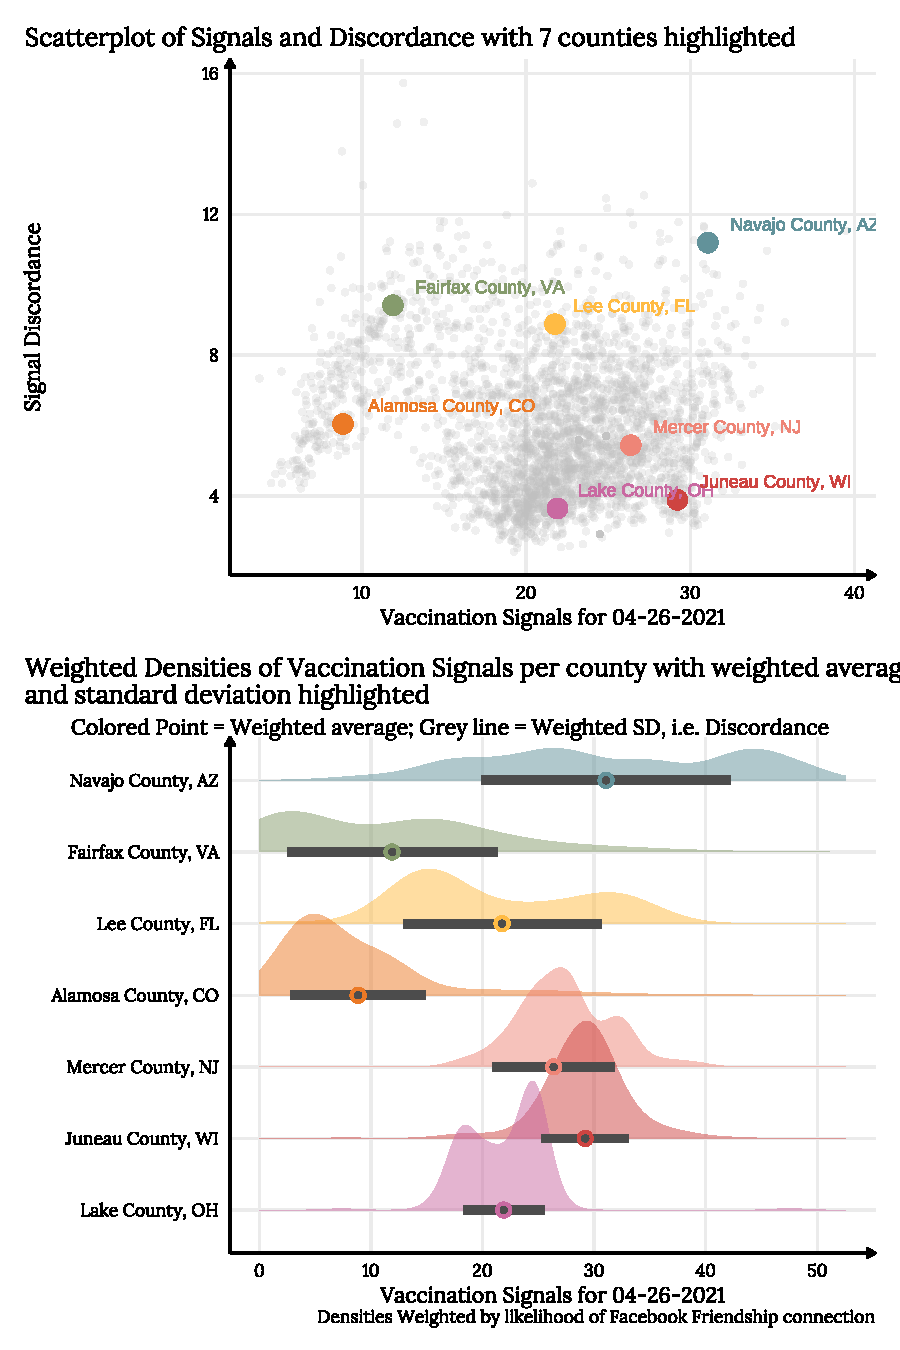
\includegraphics[width=0.7\linewidth]{figs/paper3/assortativity-vacc-1}}
\caption{How Network Signal and Discordance are Calculated, Sampled Regions}\label{fig:assortativity-vacc}
\end{figure}

\begin{figure}
\begin{center}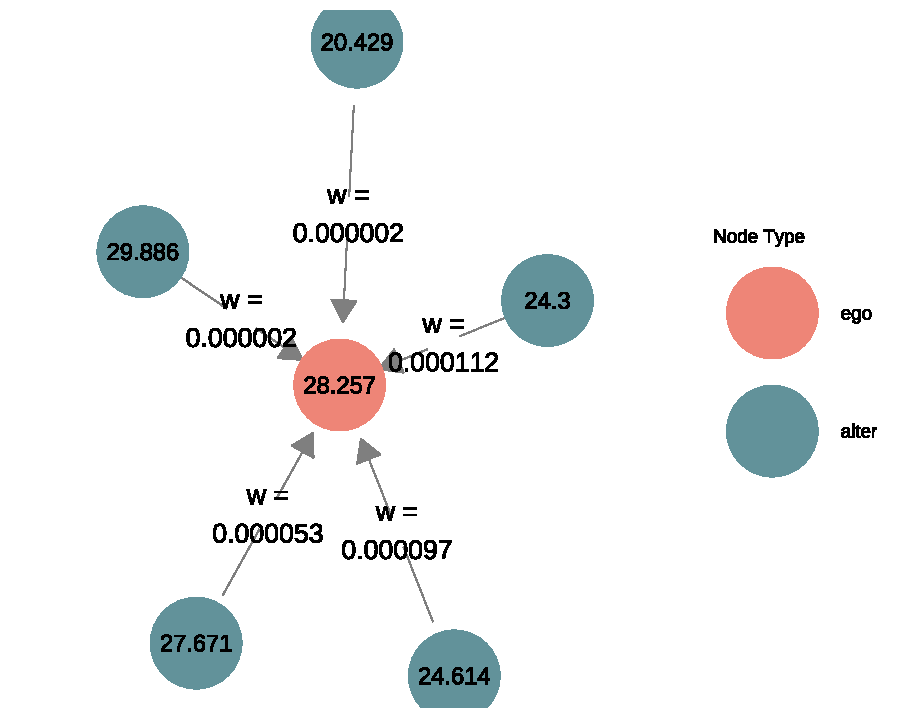
\includegraphics[width=0.5\linewidth,]{figs/paper3/discordancenetwork-1.pdf} 
  \begin{equation}
    w = \begin{bmatrix}0.0000015\\0.0000023\\0.0000527\\0.0000966\\0.0001119\end{bmatrix},  
    x = \begin{bmatrix}29.9\\20.4\\27.7\\24.6\\24.3\end{bmatrix} \longrightarrow
    \begin{matrix} \bar{x}*, signal = 25.083\\ s*, discordance = 1.423 \end{matrix} 
  \end{equation}
  \caption{How Network Signal and Discordance are Calculated, Mathematical Example}
  \label{fig:discordancenetwork}
  \end{center}
\end{figure}

\hypertarget{COVID-19-case-rates}{\subsubsection{COVID-19 Case Rates}\label{COVID-19-case-rates}}

To estimate the concept of `real threat of infection' for a fear-based model of
health behaviors, the models use county-level COVID-19 case rates with data
compiled by The New York Times \citeyearpar{covid_data}. It is widely
acknowledged that there are biases in this data due to inconsistencies and
availability in testing as well as different community propensity to test
\citep{gu22, cdc20a}. However, it is the best measure we have of actual case
rates. County data are scaled with a rolling mean with a rolling window width of
seven days to smooth out intra-week noise. Case Rate is measured as number of
cases per 100,000 population. Observations vary from a minimum of 0 to a maximum
of 1,565 across the two datasets.

\hypertarget{online-norms}{\subsubsection{Online Norms}\label{online-norms}}

To operationalize the search for online norms, I use Google search trends
\citep{googletrends}. In \hyperlink{paper-1}{Article 1}, I show
that Google Search Trends can only be used to indicate interest due to their low
criterion validity \citep{jungherr_etal17}. I use Google Trends over the study
period across individual designated media markets areas (DMAs), a nonoverlapping
aggregation of U.S. counties to 210 media markets based on similar population
clusters \citep{dma_key}. To investigate the rate of \emph{searching} for norms
online in both cases, I use the following search topics: `Social Distancing'
(2020, stay-at-home case only), `COVID-19 Vaccine' (2021, vaccination uptake
case only) and Covid Conspiracy (2020-2021, both cases). Search topics are a
more robust measurement than a single search term: topics are aggregations of
the rates of multiple, highly correlated search terms together into a cohesive
topic. For example, while `Beyoncé,' `Beyonce' and `beyonce knowles' are all
separate search terms, `Beyoncé Knowles' encompasses all of these into a single
search topic. While the data is originally on a scale of 0 to 100, with 100
being the maximum search popularity out of all DMAs, Google Search Trend are now
only available cross-sectionally (a single time period across a geography) or
time-series (a single geo-location across time). To remedy this and build a
longitudinal dataset of each search topic, I follow the method proposed in
\citet[p. 5]{park_etal}. This method involves building a dataset of unscaled
cross-sectional values, selecting a DMA to use to establish the rescaling ratio
(I use `Los Angeles CA'), and then finding the time-series values for the one
DMA. To find the rescaling ratio for each week in the time-series, you divide
the time-series value for each week by the cross-sectional value for each week,
resulting in a rescaling vector to be used for all weeks in the dataset across
geographies. To rescale each longitudinal value, multiply the respective week's
rescaling ratio by the cross-sectional value. Rescaled longitudinal data was
compared against time-series data for multiple test counties and was equivalent.
For a more in-depth explanation of this procedure, see \citet[p. 5]{park_etal}.

\hypertarget{pillars-of-convervatism}{\subsubsection{Pillars of Convervatism}\label{pillars-of-convervatism}}

Research has shown that stay-at-home rates and other pandemic health behaviors
are related to various `pillars of conservatism'
\citep{gonzalez_etal21,hillBloodChristCompels2020,hillLoveThyAged2021,
hillNastiestQuestion}. Namely, research shows that politically conservative
indicators, such as Republican political leadership, conservative Protestantism
and consumption of right-wing media are related to higher rates of movement and
lower rates of mask usage. Based on these findings, this article controls for
these factors in the following ways: to measure Republican political leadership,
I include percentage of votes for Donald Trump in the previous presidential
election; for the 2020 study, I use the 2016 results and for the 2021 study, I
use the 2020 results to infer proper time ordering. Second, to measure
conservative Protestantism, I employ the county's percentage of evangelical
Christians. These county-level data were collected through the 2010 U.S.
Religion Census: Religious Congregations and Membership Study
\citep{grammich_etal18}. Finally, right-wing media consumption is assessed using
Google Search Trends to capture ``Fox News'' searches over the study period
across individual designated media markets areas (DMAs). I use this measure to
indicate active interest in and attention toward Fox News. While Google Search Trends
have been validated for use in a range of research contexts and for use with
survey data, voting data, and ecological data
\citep{bailPrestigeProximityPrejudice2019, reyesUsingInternetSearch2018,
scheitleGoogleInsightsSearch2011, stephensdavidowitzCostRacialAnimus2014,
swearingenGoogleInsightsSenate2014}, I provide a caution for these uses in 
\hyperlink{paper-1}{Appendix A} and suggest these measures should only be used to measure attention. 


\hypertarget{demographics}{\subsubsection{Demographics}\label{demographics}}

These models also control for (1) percent of the population that is above 65
years old (those most at risk of hospitalization), (2) percent of the population
that identifies as white, (3) percent of the population that holds a college
degree, (4) median income, and (5) monthly county unemployment rate. Measures 1
through 4 are obtained from the 2018 American Community Survey: 5-Year Estimates
\citep{uscensusbureauAmericanCommunitySurvey2018}; unemployment rates are
gathered from the U.S. Bureau of Labor Statistics \citep{labor2020a}.

\hypertarget{analysis-and-results}{\section{Analysis and Results}\label{analysis-and-results}}

My analytic strategy proceeds in four steps. In Tables
\ref{tab:google-desc-table} (Stay-at-Home) and \ref{tab:vacc-desc-table}
(Vaccination Uptake), I present descriptive statistics for all study variables,
including variable ranges, means, and standard deviations across the two cases.
Then, in Tables \ref{tab:google-tab} - \ref{tab:vacc-tab}, I fit a series of
three linear mixed effects regression models using the nlme package in R
\citep{pinheiro_etal21, pinheiro_bates00} for our two cases, Stay-at-Home rates
and Vaccination rates. Linear mixed effects models are a form of hierarchical
linear models that contain both random and fixed effects. These models treat the
dependent variables as continuous. The following strategies I will outline are
identical for both case studies. Models 1 through 3 address hypotheses
\ref{hyp:infection} through \ref{hyp:discordance} respectively. Each model
utilizes normalized independent variables, i.e.\ variables that have been
centered and scaled to have a mean of 0 and standard deviation 1. The first
model is a baseline linear mixed effects model that employs all basic controls
to predict the dependent variable, allowing both time-varying and county-level
variables to predict the outcome. All variables have fixed effects, meaning that
the county-level exogenous effects are controlled for when estimating the
coefficient. In addition, models are specified with a random intercept per
county. The lme models are set with a autoregressive correlation structure
(\texttt{correlation\ =\ corAR1()}) to control for temporally autocorrelated
error structures; models are also optimized using Nelder--Mead, quasi--Newton and
conjugate--gradient algorithms for box-constrained optimization and simulated
annealing (\texttt{control\ =\ lmeControl(opt\ =\ ``optim'')}). This first model
will address Hypothesis \ref{hyp:infection}. To test Hypothesis
\ref{hyp:direction}, I estimate model 2 which builds on model 1 by first
introducing vaccination signal. Because the signal varies by week, I estimate
this model with an interaction between week and signal. And finally, because
signal may have divergent effects across counties, I set a random effect for
signal nested by county. A visual representation of this interaction can be seen
in Figures \ref{fig:plot-google-h2} and \ref{fig:plot-vacc-h2}. Model 3 further
elaborates on the previous model by introducing both a fixed effect for signal
discordance and an interaction term between signal and discordance. Figures
\ref{fig:plot-google-h3} and \ref{fig:plot-vacc-h3} depict just how signal and
discordance interact across these two cases.

\hypertarget{stay-at-home-rate-results}{
\subsection{Stay-at-Home Rate results}\label{stay-at-home-rate-results}}

\begin{table}[!h]

\caption{\label{tab:google-tab}Linear Mixed Effects Regression Results for Stay-At-Home Rates}
\centering
\fontsize{8}{10}\selectfont
\begin{tabular}[t]{lccc}
\toprule
  & Model 1 & Model 2 & Model 3\\
\midrule
Percent White & \num{0.088}*** & \num{0.058}** & \num{0.060}**\\
 & (\num{0.023}) & (\num{0.019}) & (\num{0.019})\\
Percent College Graduates & \num{-0.016} & \num{0.010} & \num{0.020}\\
 & (\num{0.028}) & (\num{0.023}) & (\num{0.024})\\
Percent over 65 & \num{-0.034}+ & \num{-0.031}* & \num{-0.037}*\\
 & (\num{0.018}) & (\num{0.015}) & (\num{0.015})\\
Median Income & \num{-0.042} & \num{-0.032} & \num{0.015}\\
 & (\num{0.030}) & (\num{0.024}) & (\num{0.025})\\
Monthly Unemployment Rate & \num{0.087}*** & \num{0.012}*** & \num{0.065}***\\
 & (\num{0.003}) & (\num{0.003}) & (\num{0.004})\\
Percent of GOP votes, 2016 & \num{0.077}* & \num{0.043} & \num{0.017}\\
 & (\num{0.032}) & (\num{0.026}) & (\num{0.027})\\
Percent Evangelical Christian & \num{-0.016} & \num{-0.008} & \num{-0.014}\\
 & (\num{0.022}) & (\num{0.018}) & (\num{0.019})\\
'Fox News' Trend & \num{-0.030}*** & \num{-0.028}*** & \num{-0.026}***\\
 & (\num{0.001}) & (\num{0.001}) & \vphantom{1} (\num{0.001})\\
'Social Distancing' Trend & \num{0.011}*** & \num{0.004}* & \num{0.001}\\
 & (\num{0.002}) & (\num{0.002}) & \vphantom{1} (\num{0.002})\\
'Covid Conspiracy' Trend & \num{0.024}*** & \num{0.006}*** & \num{0.010}***\\
 & (\num{0.002}) & (\num{0.002}) & (\num{0.002})\\
Covid Case Rate & \num{0.000} & \num{-0.009}* & \num{-0.007}+\\
 & (\num{0.004}) & (\num{0.004}) & (\num{0.004})\\
Week Number & \num{-0.002}+ & \num{-0.002}* & \num{-0.004}***\\
 & (\num{0.001}) & (\num{0.001}) & (\num{0.001})\\
Stay at Home Rate, county mean & \num{0.898}*** & \num{0.873}*** & \num{0.846}***\\
 & (\num{0.059}) & (\num{0.048}) & (\num{0.050})\\
Signal &  & \num{0.473}*** & \num{0.550}***\\
 &  & (\num{0.005}) & (\num{0.008})\\
Signal x Week &  & \num{-0.016}*** & \num{-0.018}***\\
 &  & (\num{0.000}) & (\num{0.000})\\
Signal Discordance &  &  & \num{-0.101}***\\
 &  &  & (\num{0.004})\\
Signal x Signal Discordance &  &  & \num{-0.092}***\\
 &  &  & (\num{0.002})\\
\midrule
Log.Lik. & \num{-23007.044} & \num{-19555.920} & \num{-18655.837}\\
\bottomrule
\multicolumn{4}{l}{\rule{0pt}{1em}N = 57,356, N of random Effects = 1375}\\
\multicolumn{4}{l}{\rule{0pt}{1em}* p $<$ .05. ** p $<$ .01. *** p $<$ .001 (two-tailed test).}\\
\multicolumn{4}{l}{\rule{0pt}{1em}Model 1 includes a random intercept for FIPS,}\\
\multicolumn{4}{l}{\rule{0pt}{1em}Models 2-3 include a random effect for Movement Signal by FIPS}\\
\end{tabular}
\end{table}


In Table \ref{tab:google-tab} and Figures \ref{fig:plot-google-h2} -
\ref{fig:plot-google-h3}, I present the elaboratory county-level models that
predict stay-at-home rates, or, time spent in residence. Model 1 addresses
Hypothesis \ref{hyp:infection}, that relatively higher local rates of infection
will lead to increased time spent in residence. This model's phi parameter is
0.933, which is a good indicator that adjacent time points for each county are
related and the model is specified correctly (Finch, Bolin, and Kelley 2014). In
this first model, many controls have an impact on the outcome. For instance,
when controlling for everything else, the percent of GOP votes in 2016, the
percentage of residents who identify racially as White, and higher rates of
unemployment increased the stay-at-home rate while Searches for norms online
seems to have an effect on the outcome: searches for `Fox News' are associated
with decreased stay-at-home rates, while searching for both `Social Distancing'
and `Covid Conspiracy' tend to increase time spent in residence. Interestingly,
the perceived threat of the virus, measured through COVID-19 case rates, were
not significantly related to stay-at-home rates in model 1. In other words, for
every 1 standard deviation increase in COVID-19 case rates, stay-at-home rates
actually decreased by 0.0003 (\emph{p} = 0.936), a very small and insignificant
effect. In this case, I fail to reject the null hypothesis that relatively
higher local rates of infection will lead to increased time spent in residence.

Table \ref{tab:google-tab} Model 2 investigates Hypothesis \ref{hyp:direction},
that increased average time spent in residence (signal direction) from alters
will have a positive effect on stay-at-home rates for the ego-county. This model
builds on model 1 by adding in the variable for Movement Signal (see
\protect\hyperlink{network-signal}{Network Signal} for specifications). For
every one standard deviation increase in the average time spent in residence of
the county alters, an ego tends to also increase its' own stay-at-home rate by
0.473 (\emph{p} \textless{} 0.001). I am therefore able to reject my null
hypothesis for Hypothesis \ref{hyp:direction}, that an increased average time
spent in residence (signal direction) from alters will have a positive effect on
time spent in residence for the ego-county.

\begin{figure}
{\centering 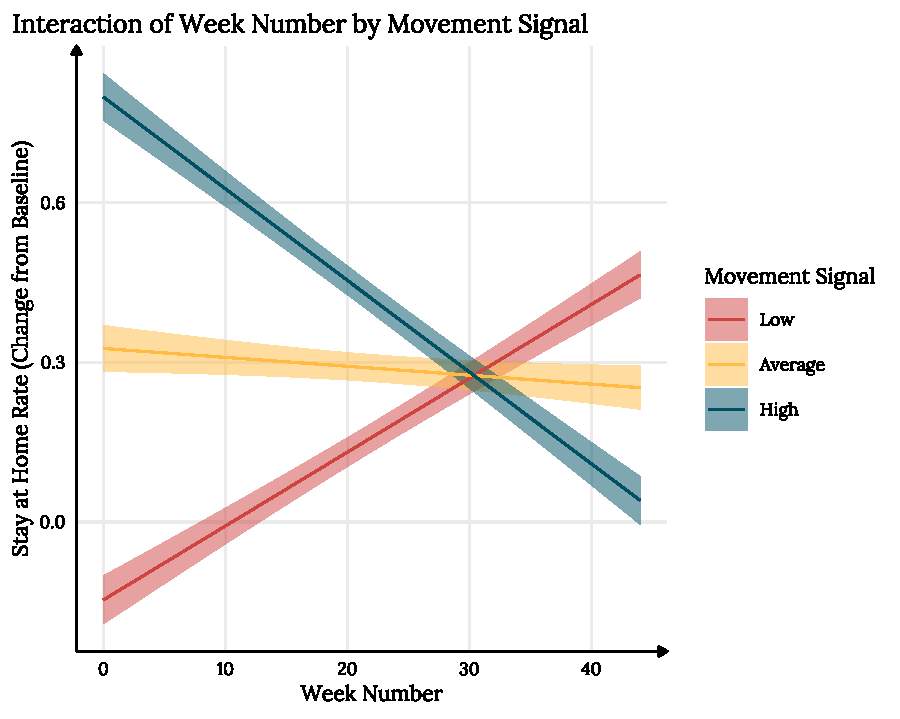
\includegraphics[width=0.8\linewidth]{figs/paper3/plot-google-h2-1}}
\caption{Predicted Values of Stay-at-Home Rate by Movement Signal, Model 2}\label{fig:plot-google-h2}
\end{figure}

However, this coefficient is inadequate alone because the effect varies over
time; the interaction between week and movement signal is negative, meaning that
week partially moderates the effect of the signal. Figure
\ref{fig:plot-google-h2} illustrates this interaction. In the early days of the
COVID-19 pandemic, seeing a high rate of time spent in residence by alters led
to a high rate of staying-at-home for county egos. However, as the pandemic
progressed, these signals switched. In other words, towards the end of 2020,
other factors may have come into play and if a county saw its' alters social
distancing and spending time in residence, ego counties spent less time at home.
Theoretically, this may be because individuals saw their adjacent communities
with strong public health norms and felt safe and justified their own deviance.
However, if an ego county received signals that others were failing to social
distance, they were more likely to stay-at-home. In this case, the threat of the
virus may have been more evident for individuals.

\begin{figure}
{\centering 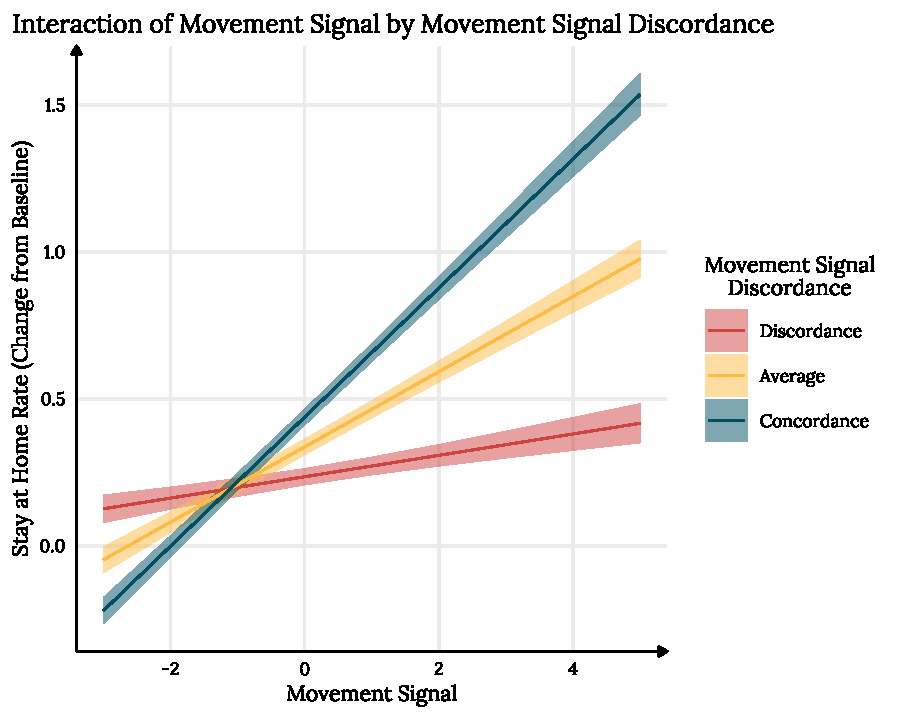
\includegraphics[width=0.8\linewidth]{figs/paper3/plot-google-h3-1}}
\caption{Predicted Values of Stay-at-Home Rate Moderated by Discordance, Model 3}\label{fig:plot-google-h3}
\end{figure}

Model 3 then adds the concept of Signal Discordance to investigate Hypothesis
\ref{hyp:discordance}, that the effect of signal direction on stay-at-home rates
will be moderated by a diversity in signals (\emph{discordance}). Many of the
controls remain consistent throughout the models, with the exception of `Social
Distancing' Trend whose effect has been completely mediated by the inclusion of
signal discordance. Importantly, signal discordance has a negative effect on
stay-at-home rates, where every one standard deviation increase in discordance
lowers stay-at-home rates by -0.101 (\emph{p} \textless{} 0.001). The
interaction between signal and signal discordance have a coefficient of a
similar magnitude, with every one standard deviation increase in discordance and
signal resulting in -0.092 lower rates of time spent in residence, indicating
moderation. Figure \ref{fig:plot-google-h3} illustrates the moderating effect
that signal discordance has on signal. Under high discordance, the social
influence effect is almost completely moderated because there is no clear story
or norm forming. However, under low discordance, the signal is condensed,
allowing for social influence to have an effect. Explicitly, if a county is
receiving a wide array of low and high signals, their stay-at-home rates won't
be affected on average by social contagion. When a signal is concentrated or in agreement,
the theoretical effect of movement signaling on the ego are the strongest. With
this, I am able to reject the null hypothesis of no relationship for Hypothesis
\ref{hyp:discordance} and find that the effect of signal direction on time spent
in residence is moderated by diversity in signals.

\hypertarget{vaccination-rate-results}{\subsection{Vaccination Rate results}\label{vaccination-rate-results}}

\begin{table}[!ht]

\caption{\label{tab:vacc-tab}Linear Mixed Effects Regression Results for Vaccination Rates}
\centering
\fontsize{8}{10}\selectfont
\begin{tabular}{lccc}
\toprule
  & Model 1 & Model 2 & Model 3\\
\midrule
Percent White & \num{0.023}+ & \num{-0.029}*** & \num{-0.027}***\\
 & (\num{0.012}) & (\num{0.003}) & (\num{0.003})\\
Percent College Graduates & \num{-0.004} & \num{0.009}* & \num{0.010}*\\
 & (\num{0.013}) & (\num{0.004}) & (\num{0.004})\\
Percent over 65 & \num{-0.012} & \num{-0.002} & \num{0.000}\\
 & (\num{0.008}) & (\num{0.002}) & (\num{0.002})\\
Median Income & \num{0.002} & \num{-0.017}*** & \num{-0.016}***\\
 & (\num{0.011}) & (\num{0.003}) & (\num{0.003})\\
Monthly Unemployment Rate & \num{-0.031}*** & \num{-0.014}*** & \num{-0.013}***\\
 & (\num{0.001}) & (\num{0.001}) & (\num{0.001})\\
Percent of GOP votes, 2020 & \num{-0.070}*** & \num{0.031}*** & \num{0.028}***\\
 & (\num{0.014}) & (\num{0.004}) & (\num{0.004})\\
Percent Evangelical Christian & \num{0.000} & \num{0.000} & \num{-0.001}\\
 & (\num{0.009}) & (\num{0.003}) & (\num{0.003})\\
'Fox News' Trend & \num{0.002}*** & \num{0.000} & \num{0.000}*\\
 & (\num{0.000}) & (\num{0.000}) & \vphantom{4} (\num{0.000})\\
'Vaccine' Trend & \num{-0.001}*** & \num{0.000} & \num{0.000}+\\
 & (\num{0.000}) & (\num{0.000}) & \vphantom{3} (\num{0.000})\\
'Covid Conspiracy' Trend & \num{0.000}* & \num{0.001}*** & \num{0.001}***\\
 & (\num{0.000}) & (\num{0.000}) & \vphantom{2} (\num{0.000})\\
Covid Case Rate & \num{-0.008}*** & \num{0.001}*** & \num{0.001}***\\
 & (\num{0.000}) & (\num{0.000}) & \vphantom{1} (\num{0.000})\\
Week Number & \num{0.067}*** & \num{0.011}*** & \num{0.011}***\\
 & (\num{0.000}) & (\num{0.000}) & (\num{0.000})\\
Vaccination Rate, county mean & \num{0.800}*** & \num{0.201}*** & \num{0.170}***\\
 & (\num{0.018}) & (\num{0.005}) & (\num{0.005})\\
Vaccination Signal &  & \num{0.854}*** & \num{0.865}***\\
 &  & (\num{0.005}) & (\num{0.006})\\
Vaccination Signal x Week &  & \num{-0.005}*** & \num{-0.003}***\\
 &  & (\num{0.000}) & (\num{0.000})\\
Vaccination Discordance &  &  & \num{-0.072}***\\
 &  &  & \vphantom{1} (\num{0.002})\\
Vaccination Signal x Discordance &  &  & \num{-0.051}***\\
 &  &  & (\num{0.002})\\
\midrule
Log.Lik. & \num{118677.013} & \num{160000.978} & \num{160638.703}\\
\bottomrule
\multicolumn{4}{l}{\rule{0pt}{1em}N = 99,890, N of random Effects = 2819}\\
\multicolumn{4}{l}{\rule{0pt}{1em}* p $<$ .05. ** p $<$ .01. *** p $<$ .001 (two-tailed test).}\\
\multicolumn{4}{l}{\rule{0pt}{1em}Model 1 includes a random intercept for FIPS,}\\
\multicolumn{4}{l}{\rule{0pt}{1em}Models 2-3 include a random effect for Movement Signal by FIPS}\\
\end{tabular}
\end{table}

In Table \ref{tab:vacc-tab} and Figures \ref{fig:plot-vacc-h2} -
\ref{fig:plot-vacc-h3}, I present the elaboratory county-level models that
predict vaccination uptake rates. The parameter phi in model 1 is .985, which is
a good indicator that adjacent time points for each county are related and this
is an appropriate modeling technique for the data \citep{finch_etal14}. Table
\ref{tab:vacc-tab} Model 1 addresses Hypothesis \ref{hyp:infection}, that
relatively higher local rates of infection will lead to increased vaccination
uptake. In this first model, we see various controls impacting vaccination
rates. For instance, when controlling for everything else, higher income areas
lead to higher vaccination uptake. On the other hand, counties with higher
unemployment and higher votes for Donald J. Trump in the 2020 election are
associated with lower vaccination rates. Interestingly, counties that search for
Fox News are more likely to have higher vaccination rates while those performing
Google searches for information about the vaccine are likely to have lower rates
of vaccination. 
% TODO On the Fox News result--Interesting. In hindsight, this too may have to do with inhomogeneities within counties, e.g., maybe it's the conservatives in liberal counties that tune in avidly to Fox News.
The test of Hypothesis \ref{hyp:infection} also returns
surprising results: every 1 standard deviation increase in county COVID-19 case
rates is expected to yield a -0.008 decrease in vaccination rates. This may be
due to time ordering or reverse causality, where individuals in counties who
have higher rates of vaccination are less likely to take tests to COVID-19
infections because of the higher likelihood of asymptomaticity. However, it is
important to note that the Case Rate variable actually becomes distorted with
the addition of Vaccination Signal and Vaccination Discordance in models 2 and
3. Distortion occurs when the direction of a focal relationship reverses sign
once a third (distorter) variable is controlled, in this case, those related to
signal. Therefore, the results of Hypothesis \ref{hyp:infection} are quite
inconclusive.
% TODO Those who perform Google searches for vaccine info are likely to have lower vaccination rates --> Maybe they are searching for info about why the vaccine is bad !!

% TODO An increase in covid cases yields a decrease in vaccination rates. -- Well, the association would be like this if low vaccination rates lead to more covid cases.

\begin{figure}
{\centering 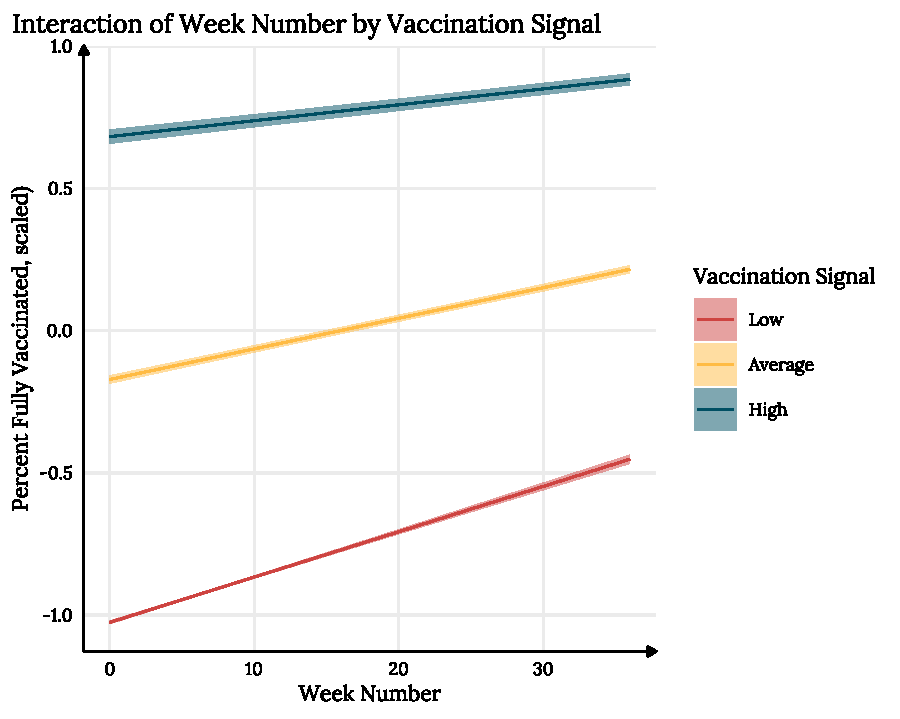
\includegraphics[width=0.8\linewidth]{figs/paper3/plot-vacc-h2-1}}
\caption{Predicted Values of Vaccination Rate by Vaccination Signal, Model 2}\label{fig:plot-vacc-h2}
\end{figure}

Table \ref{tab:vacc-tab} model 2 tests the Hypothesis \ref{hyp:direction} that
increase vaccine uptake by alters will have a positive effect on vaccine uptake
for the ego-county. The results are incredibly clear: seeing alter counties
receiving vaccines is associated with higher vaccination rates. Specifically, a
1 standard deviation increase in vaccine signal, the average rate of vaccination
of a county's alters, is associated with a 0.854 percent increase of vaccination
rates for the ego county. The strength of this result leads me to reject the
null hypothesis for Hypothesis \ref{hyp:direction} and find that increased
average time spent in residence (signal direction) from alters will have a
positive effect on time spent in residence for the ego-county. The interaction
of vaccine signal can be seen in Figure \ref{fig:plot-vacc-h2}. While the
interaction is not as extreme as the results for Hypothesis \ref{hyp:direction}
for Stay-at-Home rates, there is still a distinction between high and low
vaccination signals over time. The slope for Higher Vaccination Signal is less
pronounced than Low Vaccination Signal. This is likely an artifact where some
counties vaccinated broadly early on, so their vaccination rate stays rather
constant in later weeks. However, overall, the message is clear: ego-counties
who `see' high levels of vaccinations among their alters have higher vaccination
rates; those who don't see that social norm forming are much less likely to
vaccinate.

\begin{figure}
{\centering 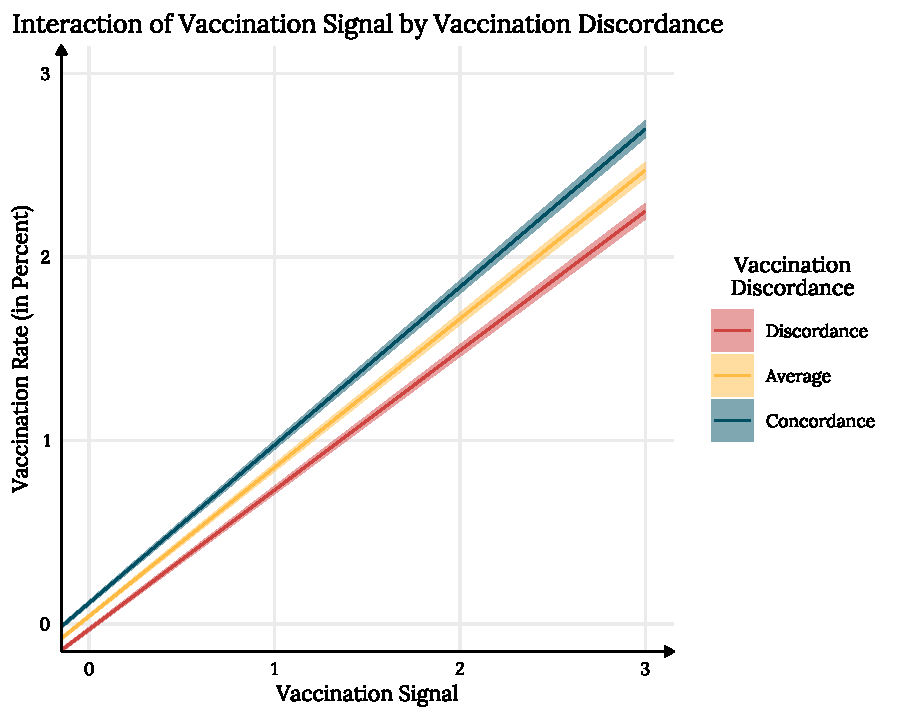
\includegraphics[width=0.8\linewidth]{figs/paper3/plot-vacc-h3-1}}
\caption{Predicted Values of Vaccination Rate Moderated by Discordance, Model 3}\label{fig:plot-vacc-h3}
\end{figure}

Table \ref{tab:vacc-tab} Model 3 then models the moderation of signal direction
for vaccine uptake by diversity in signals (\emph{Discordance}). This is a
second test of Hypothesis \ref{hyp:discordance}, that the effect of signal
direction on vaccine uptake will be moderated by diversity in signals. The
coefficients in model 3 are largely consistent with model 2 and there is very
little change in the magnitude or significance of the coefficients. Vaccination
signal maintains to have a positive effect on the alter's vaccination rates,
while vaccination discordance has a negative effect on vaccination rates, where
every one standard deviation increase in discordance lowers rates by -0.072
(\emph{p} \textless{} 0.001). The interaction between signal and signal
discordance have a coefficient of a similar magnitude, with every one standard
deviation increase in discordance \emph{and} signal resulting in lower rates of
vaccination. Figure \ref{fig:plot-vacc-h3} illustrates this relationship, where
there is slight moderation of the effect on vaccine signal on vaccination rates.
If a county receives consistently high signals, they are more likely to have
more residents vaccinated. If a county receives high but inconsistent signals,
they are still decently likely to raise vaccination rates but to a lesser
extent. While not as strong of moderation the the findings for Stay-at-Home
Rates for Hypothesis \ref{hyp:discordance}, I also reject the null hypothesis
and find a moderation of the relationship between signal direction and vaccine
uptake by discordance.

\hypertarget{discussion-and-conclusion}{\section{Discussion and Conclusion}\label{discussion-and-conclusion}}

This paper examines how social norms are formed under conditions of uncertainty
using the case studies of stay-at-home rates and vaccination rates during the
COVID-19 pandemic. I test fear-based models of behavioral adaption to public
health recommendations as well as patterns of complex social contagion. This
article demonstrates that the establishment of social norms under patterns of
uncertainty in my two cases do follow the theorized framework of complex
contagion; however, I find a moderating effect of signal discordance to be an
overlooked factor in theories of contagion.

This study is sensitive to aggregation error and sampling error derived from the
multiple big-data sources \citep{facebook20, google2020}. The aggregation errors
are potentially linked to the assumption that the average stay-at-home behavior
of a county is a good representation of the diversity in behaviors within that
county. If stay-at-home rates are normally distributed, this is a correct
assumption to make; however, little is known about each county's underlying
distribution of behaviors that lead to the aggregate measures.
% TODO As perhaps illustrated hypothetically in my comment on p. 120

Despite limitations, this article is a unique and compelling contribution
to the academic study of social contagion and social norms. First, this article
demonstrates that it is possible to link, at least at a community level,
information search by individuals, social relationships, and observed health
behaviors without being limited to self-report measures of perceptions,
attitudes, or intentions about behavior. Sociological research has long debated
about the agency of individuals and the social and institutional structure in
which individuals are immersed. In this study, I aggregate beyond the individual
case to explore overall patterns of movement and vaccination which summarizes
individual agency of health behaviors together.

This article also provides a new adaption of the theory of complex contagion
using big data from the natural experiment of COVID-19. Because most studies of
complex contagion utilize agent-based modeling or studies of social media
\citep{aralExerciseContagionGlobal2017,sprague_house17,bond_etal12,latane_etal94},
combining measures of actual behavioral outcomes with data from social media
websites provides a further test of ecological and external validity for the
theory.

Researchers of contagion and social networks should be interested in this study.
My theory of discordance, or a diversity of signals received, is not found in
the literature on complex contagion; complex contagion focuses on the number of
reinforcing actors, while other theories focus on how different diffusants
interact with each other
\citep{houghton20,goldbergSocialContagionAssociative2018,mason_etal07}.
Discordance, on the other hand, looks specifically at the context of the
reinforcing actors among the other signals. This study finds that indeed the
context of the signals matters for diffusion.
\newpage
\section{References}
\begin{singlespace}
\printbibliography[heading=none] % print section bibliography
\end{singlespace}
\end{refsection}

\end{document}
